\documentclass{report}
\usepackage[a4paper, total={6in, 9in}]{geometry}
\usepackage{graphicx} % Required for inserting images
\graphicspath{ {./images/} }
\usepackage{caption}
\usepackage{subcaption}
\usepackage{pgfplotstable}
\usepackage{minitoc}
\usepackage{xcolor} % For coloring
\usepackage{amsmath} 

% \usepackage{titlesec}
% \usepackage{amsthm}
% \usepackage{cleveref}

\usepackage{setspace}
% \doublespacing
\onehalfspacing

%Bibliography
% \usepackage{natbib}
% \bibliographystyle{plainnat}
\usepackage[backend=biber, style=apa, sorting=none]{biblatex}
\addbibresource{biblio_zotero_15072025.bib}

\newcommand{\citep}{\parencite}
\newcommand{\citet}{\textcite}

\pgfplotsset{compat=1.18}

\usepackage{xspace}
\newcommand{\native}{\textit{interp\_topo}\xspace}
\newcommand{\std}{\textit{subgrid\_halfdeg}\xspace}
\newcommand{\noirr}{\textit{no\_irr}\xspace}
\newcommand{\irr}{\textit{irr}\xspace}
\newcommand{\irrboost}{\textit{irr\_boost}\xspace}
\newcommand{\betairrig}{$\beta_{irrig}$\xspace}
\newcommand{\presnoirr}{\textit{present\_no\_irr}\xspace}
\newcommand{\futnoirr}{\textit{future\_no\_irr}\xspace}
\newcommand{\futirr}{\textit{future\_irr}\xspace}
\newcommand{\smalld}{\textit{small\_domain}\xspace}
\newcommand{\interd}{\textit{intermediate\_domain}\xspace}
\newcommand{\larged}{\textit{large\_domain}\xspace}
\newcommand{\forcingERA}{\textit{forcing\_ERA}\xspace}
\newcommand{\forcingICO}{\textit{forcing\_ICOLMDZOR}\xspace}

\newcommand{\forcingoneh}{\textit{forcing\_1h}\xspace}
\newcommand{\forcingsixh}{\textit{forcing\_6h}\xspace}
\newcommand{\atmchapters}{Chapters \ref{chap:forcing}, \ref{chap:monthly}, and \ref{chap:liaise}\xspace}

% \newcommand{\tcst1}{\textit{TCST\_1}\xspace}
% \newcommand{\tcst2}{\textit{TCST\_2}\xspace}
% \newcommand{\tcst3}{\textit{TCST\_3}\xspace}
% \newcommand{\tcst4}{\textit{TCST\_4}\xspace}
%units
\newcommand{\perday}{d$^{-1}$\xspace}
\newcommand{\persqm}{m$^{-2}$\xspace}


\usepackage{hyperref}
\usepackage{booktabs} %doesn't work ? 

\begin{document}

\begin{titlepage}
    \centering
    \vspace*{2cm}

    {\Huge\bfseries Modelling regional impacts of irrigation on climate, the water cycle, and the atmospheric boundary layer over the Iberian Peninsula\par}
    \vspace{1cm}

    {\Large Pierre Tiengou\par}
    \vspace{0.5cm}

    {\large Sorbonne Université\par}
    \vspace{0.5cm}

    {\large 01/12/2025\par}

    \vfill
    
    {\large Composition du jury \par
        Mme Fabienne LOHOU \\
        Mme Isabelle BRAUD \\
        M. Jean-Louis DUFRESNE \\
        M. Romain ROEHRIG \\
        M. Martin BEST \\
        M. Aaron BOONE \\
        Mme Agnès DUCHARNE \\
        Mme Frédérique CHERUY\\
    }


    % \includegraphics[width=0.3\textwidth]{logo.png}
\end{titlepage}

\section*{Abstract}

Irrigation is a widespread agricultural practice expected to keep expanding in the future. It is recognized as a major anthropogenic driver of land-atmosphere interactions, significantly affecting regional climate, continental and atmospheric water cycle components, surface energy balance, and the atmospheric boundary layer (ABL).
Under climate change, in semi-arid regions like most of the Mediterranean basin, it is associated with major challenges regarding water availability, increased evaporative demand, and disrupted precipitation patterns, justifying efforts to understand and represent the diversity of its impacts.

This thesis investigates the effects of irrigation on the water cycle, regional climate, and the atmospheric boundary layer over the Iberian Peninsula using the ICOLMDZOR limited area model (LAM). This new regional climate model stems from the global Institut Pierre-Simon Laplace climate model (ISPL-CM), using the ORCHIDEE land surface model with a new routing scheme, the ICOLMDZ atmospheric model, and lateral forcings from ERA5 reanalyses.
It is evaluated over the region, and simulations with and without irrigation are compared to isolate its impacts.

This work first demonstrates the dominant influence of irrigation on the ability of the land surface model to simulate river discharge in offline simuulations. It identifies a more appropriate set of parameters for the river routing and irrigation scheme over the Iberian Peninsula, to adapt to a 1-arcminute resolution topography and better reflect regional irrigation practices. 
Then, in coupled LAM simulations, atmospheric impacts of irrigation mainly consist in a cooling and moistening over irrigated areas and a stabilization of the ABL. Partial recycling of atmospheric moisture is identified at the scale of the Peninsula, with increases in precipitation in mountainous regions surrounding the intensely irrigated Ebro Valley.
The atmospheric processes at play are analysed in more details by comparing the ICOLMDOZR LAM to observations data from the Land Surface Interactions with the Atmosphere over the Iberian Semi-Arid Environment (LIAISE) campaign in the Ebro valley, and Meso-NH simulations at 2-kilometer resolution over the LIAISE study area.
In a sensitivity experiment with increased water availability for irrigation, surface fluxes are found to be greatly improved compared to observations. Surface variables in the ICOLMDZOR grid cell for the irrigated observation site also match the average of Meso-NH grid cells contained within it, suggesting that the tiled approach of irrigation is sufficient to represent impacts at the surface. However, although the cooling and moistening effects of irrigation are found to extend vertically into the ABL, ICOLMDZOR does not achieve as good performance in ABL representation as in surface variables. This is attributed partly to the influence of subgrid heterogeneities, in surface fluxes, but also in wind speed and directionn, and to imperfect advection terms in ICOLMDZOR.

Overall, this work presents a first use-case of the new ICOLMDZOR LAM for the study of land-surface interactions at the regional scale, with visible impacts of irrigation on river discharge, precipitation, surface variables and ABL development.
Several sources of biases of the ICOLMDZOR LAM over the region are also identified and partly corrected, and possible improvements are presented for future regional climate modelling studies.

\clearpage

\section*{Résumé}

L'irrigation est une pratique agricole répandue, dont l'expansion devrait se poursuivre à l'avenir. Elle est reconnue comme une des activités anthropiques impactant fortement les interactions entre la surface terrestre et l'atmosphère, et peut significativement influencer le climat régional, le cycle de l'eau continental et atmosphérique, le bilan énergétique à la surface et la couche limite atmosphérique (CLA).
Dans le contexte du changement climatique, notamment dans les régions semi-arides du bassin méditerranéen, elle est associée à des défis majeurs de gestion des ressources en eau, d'augmentation de la demande évaporative et de perturbations des régimes de précipitations, qui justifient les efforts pour mieux comprendre et représenter la diversité de ses impacts.

Cette thèse étudie les effets de l'irrigation sur le cycle de l'eau, le climat régional et la couche limite atmosphérique au-dessus de la péninsule Ibérique, à l'aide du modèle à aire limitée (LAM) ICOLMDZOR. Ce nouveau modèle climatique régional est dérivé du modèle climatique global de l'Institut Pierre-Simon Laplace (IPSL-CM). Il utilise le modèle de surface continentale ORCHIDEE, doté d'un nouveau schéma de routage des rivières, le modèle atmosphérique ICOLMDZ, et des conditions aux limites issues des réanalyses ERA5.
Le modèle est évalué sur la région, et des simulations avec et sans irrigation sont comparées pour isoler ses impacts.

Ce travail démontre d'abord l'influence dominante de l'irrigation sur la capacité du modèle ORCHIDEE à simuler les débits. Un ensemble de paramètres pour le routage et l'irrigation est identifié, afin d'adapter le nouveau routage à une topographie à haute résolution (1 arcmin) et de mieux refléter les pratiques d'irrigation de la péninsule Ibérique.
Ensuite, dans les simulations couplées, les impacts atmosphériques de l'irrigation se manifestent principalement par un refroidissement et une humidification de l'air au dessus des zones irriguées, ainsi qu'une stabilisation de la CLA. Un recyclage partiel de l'humidité atmosphérique est identifié à l'échelle de la péninsule, avec une augmentation des précipitations dans les régions montagneuses qui entourent la vallée de l'Ebre, fortement irriguée.
Les processus atmosphériques en jeu sont analysés plus en détail en comparant le LAM ICOLMDZOR à des données d'observation issues de la campagne LIAISE (Land Surface Interactions with the Atmosphere over the Iberian Semi-Arid Environment) dans la vallée de l'Ebre, ainsi qu'à des simulations Meso-NH à une résolution de 2 kilomètres sur la zone d'étude de LIAISE.
Dans une expérience de sensibilité avec une disponibilité accrue en eau pour l'irrigation, les flux de surface sont grandement améliorés par rapport aux observations. Les variables de surface dans la maille ICOLMDZOR du site irrigué correspondent également à la moyenne des mailles Meso-NH qu'elle contient, suggérant que l'approche en mosaïque de l'irrigation est suffisante pour représenter les impacts à la surface. Cependant, bien que le refroidissement et l'humidification générés par l'irrigation se propage verticalement dans la CLA, ICOLMDZOR ne parvient pas à atteindre la même performance dans la représentation de la CLA que pour les variables de surface. Cela est attribué en partie à l'influence des hétérogénéités sous-maille, non seulement dans les flux de surface, mais aussi dans la vitesse et la direction du vent, ainsi qu'à des termes d'advection imparfaits dans ICOLMDZOR.

Dans l'ensemble, ce travail présente une première application du nouveau LAM ICOLMDZOR pour l'étude des interactions surface-atmosphère à l'échelle régionale, mettant en évidence des impacts visibles de l'irrigation sur les débits des rivières, les précipitations, les variables de surface et le développement de la CLA.
Plusieurs sources de biais du modèle ICOLMDZOR sur la région sont également identifiées et en partie corrigées, et des pistes d'amélioration sont proposées pour les futures études de modélisation climatique régionale.

\clearpage

\section*{Résumé long}
\section*{Remerciements}

\clearpage
\dominitoc
\renewcommand*\contentsname{Contents}
\tableofcontents
\newpage

\chapter{Introduction}
\label{chap:introduction}
\minitoc
\pagebreak
% \section{Land surface interactions}
Let's go.
\section{Irrigation}
Ok
\section{Intro article LAM1}
Physical processes at the interface between the soil surface and the lower atmosphere can influence meteorological 
%(air temperature, relative humidity, winds, precipitation)
and hydrological 
%(soil moisture, streamflow, surface runoff) 
variables at various spatial and temporal scales, contributing to complex feedback loops.
In areas where the transition regime described by \cite{Budyko_1956, Budyko_1974} is most frequent, soil moisture (SM) holds a central role in these processes as a main driver of evapotranspiration (ET), which conditions the partitioning of energy at the interface between land and atmosphere \citep{betts_fife_1995, seneviratne_investigating_2010}. 
 
The GLACE experiment used General Circulation Models (GCMs) to identify regions of strong land surface-atmosphere coupling between SM and precipitation, mostly in semi-arid transition regions \citep{koster_regions_2004}. This was confirmed by other modeling studies which also distinguished various mechanisms through which land surface conditions can impact the atmosphere in these coupling hotspots, and metrics to quantify them \citep{dirmeyer_terrestrial_2011, zou_precipitation_2023}.
Experiments were also implemented to isolate the response of the atmosphere to various surface conditions under a changing climate, such as GLACE-CMIP5 \citep{seneviratne_impact_2013} and identified land-atmosphere coupling processes as a major driver of the response to a global temperature rise in these hotspots \citep{berg_interannual_2015}. 
Moreover, the frequent warm bias of CMIP5 models \citep{christensen_temperature_2012, mueller_systematic_2014} was linked to underestimates of SM \citep{al-yaari_satellite-based_2019} and partly attributed to the representation of land surface-atmosphere coupling processes \citep{cheruy_combined_2013, cheruy_role_2014}, justifying ongoing research on their understanding and improvement within models.

A great source of complexity in land surface-atmosphere processes comes from the spatial heterogeneity of SM, which may derive from the diversity of vegetation, soil types, orographic features, and anthropogenic processes.
Increases in SM and ET have been associated with direct increases in precipitation (moisture recycling presented in \cite{eltahir_precipitation_1996}) in both modeling and observational studies \citep{koster_observational_2003, guo_glace_2006, wei_dissecting_2012, findell_probability_2011}, constituting a positive feedback loop. However, it can also lead to a stabilization of the Atmospheric Boundary Layer (ABL), inhibiting vertical development and convection \citep{findell_atmospheric_2003-1, ek_influence_2004}. This leads to a negative feedback loop where convective rainfall is more likely to occur over drier soil patches, also noticed in observations \citep{taylor_afternoon_2012, klein_dry_2020}. However, \cite{guillod_reconciling_2015} emphasized the importance of temporal context, showing that these precipitation over drier soils occur more often when soils are moister than usual at the regional scale.
Finally it must be noted that SM heterogeneities can affect precipitation through mesoscale circulations which can either favor or inhibit convection triggering \citep{findell_atmospheric_2003, taylor_frequency_2011, rochetin_morphology_2017}.\\

%irrigation : obs and known processes, regional modeling (with obs campaigns) and global modeling + link to my config
In particular, irrigation can create strong spatial heterogeneities in SM. Previous studies have already established that irrigation leads to an increase of the latent heat flux and a decrease of sensible heat flux on irrigated areas \citep{pokhrel_incorporating_2012}, leading to a moister and cooler atmosphere near the surface \citep{bonfils_empirical_2007}. 
In the American Midwest, \cite{nocco_observation_2019} showed that such effects could impact regional climate and even mask the rise in temperature induced by global warming. Different regional responses of precipitation were also observed, such as a decrease over irrigated areas \citep{alter_rainfall_2015} or an increase in downwind regions \citep{deangelis_evidence_2010}.

To analyze the atmospheric processes involved, regional modeling studies have often been used in complement of observational campaigns. The Great Plains irrigation experiment (GRAINEX, \cite{rappin_great_2021}) measurements and simulations with the Weather Research and Forecasting (WRF) model showed a lower ABL over irrigated areas and a reduction of existing mesoscale slope-induced circulations in the presence of irrigation \citep{rappin_landatmosphere_2022, phillips_influence_2022}. In the Ebro Valley (northern Spain), Meso-NH simulations over the area of the Land surface Interactions with the Atmosphere over the Iberian Semi-arid Environment campaign (LIAISE, \cite{boone_land_2019}) were shown to be greatly improved by representing irrigation \citep{lunel_irrigation_2024}, and also highlighted a weakening of the regional sea-breeze regime due to irrigation \citep{lunel_marinada_2024}.
\cite{lo_irrigation_2013} and \cite{yang_impact_2017} studied local and remote impacts of irrigation in California's Central Valley, showing a strengthening of the hydrological cycle, with moisture recycling at the river basin scale, whereas a similar study in Saudi Arabia identified a negative feedback loop with increases in precipitation located in a remote area \citep{lo_intense_2021}.
%option:With the WRF atmospheric model and Noah Land Surface Model (LSM), ABL and LCL lowering in Great Plains (quian 2013), heterogeneous response of precip in China (Liu 2021) 
%NB : Yang 2017 was also with WRF+Noah but not Lo2013 (CAM)
%option:kueppers_influence_2012 (not sure which model)
However, representations of irrigation in models can be very diverse, as they do not target the same objectives. For instance, \cite{lunel_irrigation_2024} uses an idealized representation that maintains SM at a certain level in irrigated areas. This type of modeling is suitable for short simulations over a limited domain but for Earth System Models (ESMs) running long simulations, water-conservative approaches are necessary. With this type of approach, \cite{leng_significant_2017} identified contrasted responses in river discharge and water table depth depending on the irrigation methods represented. 
%option: mention that GCMs cannot always go to the same level of details as regional/NWP models and therefore are forced to simplify (crop types, irrigation spatial and temporal patterns)
%option: Idea that most regional studies do not include interannual variability, usually only 1 summer or 1 field campaign (more expensive and models not designed for long runs)

At the global scale, average impacts of simulated irrigation were studied in coupled simulations \citep{sacks_effects_2009, puma_effects_2010, cook_irrigation_2015}, with effects mostly visible in irrigation hotspots such as India, Eastern China and the United States of America. This type of study also identified remote connections between irrigation in Asia and precipitation in East Africa \citep{de_vrese_asian_2016}, and moisture-importing and exporting regions \citep{wei_where_2013}.
Yet, it must be noted that only three CMIP6 models included a representation of irrigation, and \cite{al-yaari_role_2022} showed that they performed better in capturing the trends of several climate variables in irrigated areas.
Efforts are currently being pursued to better account for irrigation's impacts in ESMs, as is best illustrated by the Irrigation Model Intercomparison Project (IRRMIP), which aims at comparing the response of various models to the representation of irrigation \citep{yao_irrigation_2023}.\\
%option: extremes Thiery 2017 ? Hauser 20..
%option: \cite{guimberteau_global_2012} showed that irrigation can delay the onset of the Indian Monsoon.

It is not expected from ESMs to achieve the same level of precision as non-hydrostatic high resolution models in their accounting for irrigation, but the extent to which their representation of irrigation can impact simulated climate in irrigated regions is still not well constrained. 
In this context, this study aims at understanding which regional impacts of irrigation on surface-atmosphere couplings and the water cycle can be represented by a climate model. 
%option: idea of discriminating how much irrigation modeling improvement is needed (if most known effects are represented, more complexity is not required, if there are some obvious limits, research can focus on these aspects)
It leverages a new Limited Area Model (LAM) configuration introduced in the Institut Pierre-Simon Laplace Climate Model (IPSL-CM) to perform regional simulations with the land surface and atmospheric components of the global model, respectively ORCHIDEE \citep{cheruy_improved_2020} and ICOLMDZ \citep{dubos_dynamico-10_2015, hourdin_lmdz6a_2020}.
This configuration allows gaining insight on the parameterizations of the global model while running with a higher resolution (25 km) for lower computational costs.
%option: mention coupling with highres routing ? (not sure since details are given in Methods)
This work is based on two regional simulations (with and without irrigation) over the Iberian Peninsula between 2010 and 2022, analyzed on yearly and seasonal scales.
\section{CSI state of the art + translation}

Interactions between the land surface and the lower layers of the atmosphere have significant impacts on meteorological (air temperature and humidity, precipitation, wind) and hydrological (runoff, stream flow, soil moisture) variables at various spatial and temporal scales. This makes it a subject of interest for climate studies and a necessary component of climate or numerical weather prediction (NWP) models. This section aims to provide a state-of-the-art description of these interactions and their modeling, as well as the impacts irrigation can have on these interactions.

\subsection{Surface Water and Energy Budgets}

To understand the components of surface-atmosphere coupling, it is necessary to recall the main fluxes of matter and energy at the surface. 
Figure \ref{fig:budgets} depicts the various components of these two budgets.

\begin{figure}[ht]
    \centering
    
\includegraphics[width=\textwidth]{images/budgets_seneviratne.png}
    \caption{Surface water and energy budgets. Extracted from \cite{seneviratne_investigating_2010}}
    \label{fig:budgets}
\end{figure}

The surface water budget is defined by:
\begin{itemize}
    \item Precipitation (transfer from the atmosphere to the surface), $P$.
    \item Evapotranspiration (transfer from the surface to the atmosphere), $E$.
    \item Drainage of water in the soil to lower layers, denoted here as $R_g$.
    \item Surface runoff, $R_s$.
\end{itemize}

The equation governing the evolution of water quantity in the soil layer (denoted here as $S$) is:
\begin{equation}
    \frac{dS}{dt} = P - E - R_s - R_g
\end{equation}

The surface energy budget includes:
\begin{itemize}
    \item Shortwave radiation (SW), with an incoming term corresponding to incident solar radiation ($SW_{down}$) and an outgoing term corresponding to the directly reflected portion ($SW_{up}$).

    The difference between these two terms and the albedo of the considered surface are defined as:

    $SW_{net} = SW_{down} - SW_{up}$

    $\alpha = SW_{up}/SW_{down}$.
    \item Longwave radiation (LW), with an outgoing term corresponding to the infrared radiation emitted by the surface based on its temperature ($LW_{up}$) and an incoming term corresponding to the infrared radiation reflected or emitted by clouds and atmospheric gases reaching the surface ($LW_{down}$).

    The difference between these two terms is defined as $LW_{net} = LW_{down} - LW_{up}$.

    The net radiation is also defined as the sum of the two radiation terms: $R_{n} = SW_{net} + LW_{net}$.
    \item Sensible heat flux, which is a thermal transfer between the air and the surface, denoted as $SH$ in Figure \ref{fig:budgets}.
    \item Latent heat flux, which corresponds to the energy used to evaporate water at the surface. This energy flux is directly related to evapotranspiration (water flux) through the enthalpy of vaporization ($\lambda$), and is therefore denoted as $\lambda E$.
    \item Heat flux to the soil, which is a thermal conduction transfer between the considered surface layer and the lower soil layers, denoted as $G$.
\end{itemize}

The equation governing the evolution of energy in the surface soil layer (denoted as $H$ in Figure \ref{fig:budgets}) is:
\begin{equation}
    \frac{dH}{dt} = R_{n} - G - \lambda E - SH
\end{equation}

\subsection{Role of Soil Moisture in Surface-Atmosphere Coupling}

The term \textit{coupling} between the surface and the atmosphere encompasses multiple influences and feedbacks between the two systems. Soil moisture plays a central role in this coupling through its direct and indirect interactions with evapotranspiration, precipitation, and the surface energy budget.

\subsubsection*{Atmospheric Boundary Layer and Air Temperature}

In meteorology, the atmospheric boundary layer is defined as the lower part of the troposphere directly influenced by the presence of the surface. This layer is where shallow convection and turbulent diffusion phenomena occur, contributing to energy diffusion and mixing of the air.
The lowest part of the boundary layer, on the order of a few tens of meters, is called the surface layer. The influence of the Coriolis force is negligible compared to that of the surface, and the wind speed generally follows a logarithmic profile. The empirical similarity theory developed by Monin and Obukhov describes the mean flow, temperature, and humidity in this layer \citep{monin1954osnovnye}.
The height of the boundary layer varies during the diurnal cycle depending on air stability, which is related to the presence of vertical temperature and humidity gradients, and wind. It can measure a few tens of meters at night and up to a few kilometers during the day in arid regions \citep{garratt_review_1994}.

The distribution of energy between the two turbulent fluxes at the surface ($\lambda E$ and $SH$ in Figure \ref{fig:budgets}) plays an essential role in the development of the boundary layer. For a given net radiation $R_n$ and a nearly constant soil heat flux (e.g., over 24 hours if there is equilibrium between daytime and nighttime), the remaining energy is distributed between the two turbulent fluxes. The evaporative fraction (defined as $EF = \lambda E / R_n$) and the Bowen ratio (defined as $B = SH / \lambda E$) quantify this distribution. If the latent heat flux is very high compared to the sensible heat flux ($EF$ high, $B$ low), the air temperature in the surface layer remains low because the energy is primarily used for evapotranspiration, and the soil transfers little heat to the air. Conversely, if the Bowen ratio is high, a larger portion of the incident energy is transmitted directly to the air, leading to a higher air temperature near the surface and more pronounced development of the boundary layer \citep{betts_fife_1995}.

Moreover, soil moisture also affects the thermal properties of the soil, as wet soil has greater thermal inertia than dry soil. In contexts where the latent heat flux is limited, this can significantly impact air temperature by affecting nighttime cooling \citep{ait-mesbah_role_2015}. The absence of solar radiation at night usually leads to radiative cooling of the soil and air in the surface layer. However, for wetter soil, this cooling will be less pronounced due to higher thermal inertia. During daytime, the impact of this inertia is often negligible, and other processes dominate the evolution of air temperature. Still, on a daily average, an increase in soil moisture can lead to an increase in air temperature since nighttime cooling is less significant \citep{cheruy_role_2017}.

\subsubsection*{Coupling Between Soil Moisture and Evapotranspiration}

Soil moisture is a key factor in the description of evapotranspiration regimes initially established by \cite{Budyko_1956, Budyko_1974}. Three main regimes are identified for the evolution of the evaporative fraction $EF$. Figure \ref{fig:evap_regimes} represents these regimes.

\begin{itemize}
    \item If soil moisture is below a threshold $\theta_{WILT}$, called the wilting point, plants cannot extract water to transpire, bare soil no longer evaporates, and evapotranspiration (and thus the evaporative fraction) is zero. This first regime is called the \textbf{dry regime}.
    \item If soil moisture is above a critical threshold $\theta_{CRIT}$, soil moisture has no impact on $EF$, which is maximal. Evaporation is limited by the available incident energy, it is the \textbf{wet regime}.
    \item Between $\theta_{WILT}$ and $\theta_{CRIT}$, there is a \textbf{transition regime} where evapotranspiration is primarily conditioned by soil moisture. As in the dry regime, evapotranspiration is limited by soil moisture.
\end{itemize}

\begin{figure}[ht]
    \centering
    
\includegraphics[width=0.7\textwidth]{images/evap_regimes.png}
    \caption{Representation of different evapotranspiration regimes. Extracted from \cite{seneviratne_investigating_2010}.}
    \label{fig:evap_regimes}
\end{figure}

Through its influence on evapotranspiration, soil moisture directly impacts surface water and energy budgets, particularly the distribution of energy between turbulent fluxes. As explained earlier, this has consequences for air temperature and humidity in the surface layer.

However, there are also several the feedbacks of evapotranspiration on soil moisture. First, an increase in evapotranspiration directly leads to a decrease in soil moisture and an increase in air humidity. This contributes to reducing the vertical humidity gradient between the air and the surface, which tends to limit evaporation \citep{allen_crop_2000}, forming a negative feedback loop. It is also established that an increase in air temperature leads to higher evaporative demand \citep{jarvis_stomatal_1986}. If enough water is available in the soil, a temperature increase will increase evapotranspiration, thus decreasing soil moisture. This can form a positive feedback loop where dry soil leads to high air temperatures, resulting in even drier soil and extreme drought events \citep{quesada_asymmetric_2012}. If no more water is available or if there are no more gradients between the soil surface and the air, the feedback of air temperature on soil moisture becomes neutral, and the feedback loop is interrupted.

\subsubsection*{Coupling Between Soil Moisture and Precipitation}

The most complex processes of surface-atmosphere coupling concern the link between soil moisture and precipitation. Several opposing effects are at play.

First, the concept of atmospheric moisture recycling described in \cite{eltahir_precipitation_1996} relates an increase in evapotranspiration to an increase in precipitation. This constitutes a positive feedback loop between soil moisture and precipitation observed in both observational and modeling studies \citep{koster_observational_2003, guo_glace_2006, wei_dissecting_2012, findell_probability_2011}. However, high soil moisture can limit the vertical development of the boundary layer, inhibiting precipitation formation \citep{findell_atmospheric_2003-1, ek_influence_2004}. Under certain conditions, drier soil can favor the formation of convective systems and thus precipitation, creating a negative feedback loop \citep{klein_dry_2020}. Spatial heterogeneities in soil moisture have also been identified as factors influencing precipitation through mesoscale circulations that can either facilitate or inhibit the triggering of convection \citep{findell_atmospheric_2003, taylor_frequency_2011, rochetin_morphology_2017}.

The observational study \cite{taylor_afternoon_2012} highlighted a negative feedback with convective precipitation triggered over drier areas compared to neighboring wetter areas. This suggests that indirect processes related to boundary layer structure and heterogeneities can exceed the direct process of moisture recycling, although demonstrating causality in such observational studies remains challenging \cite{salvucci_investigating_2002, guillod_land-surface_2014}. Building on the purely spatial analysis of \cite{taylor_afternoon_2012}, a spatiotemporal analysis of correlations between soil moisture and precipitation highlighted the importance of temporally contextualizing heterogeneities \cite{guillod_reconciling_2015}. It showed that while precipitation is more frequently triggered over drier areas, it occurs on days that are wetter relative to the season and region concerned.

\subsection{Surface-Atmosphere Coupling in Climate Models}

Historically, the first general circulation models (GCMs) primarily focused on the atmosphere, with a very simplified representation of the surface. Over the past three decades, climate models (often called Earth System Models, ESMs) have distinctly represented continental surfaces by coupling an atmospheric model with a Land Surface Model (LSM). The complexity of these models has gradually increased, for example, to better account for the influence of vegetation or model carbon fluxes in ESMs.

From the perspective of an atmospheric model, latent and sensible heat fluxes at the surface constitute necessary boundary conditions for solving turbulent diffusion equations throughout the considered atmospheric column. These conditions impact essential meteorological variables such as air temperature, wind, and humidity. From the perspective of the LSM, precipitation computed in the atmospheric model constitutes a water input for the soil column, while surface layer characteristics (humidity, temperature, wind) condition evapotranspiration demand.

Various experiments have been designed to quantify the importance of surface coupling processes for atmospheric models. In particular, the GLACE experiments \cite{koster_glace_2006} compared atmospheric simulations with different prescribed soil moisture conditions to isolate the influence of soil moisture on precipitation. This led to the identification of hotspots: regions where this coupling is particularly pronounced. These are mainly semi-arid regions (Sahel, Great Plains in the United States) where the transitional evaporation regime described in Figure \ref{fig:evap_regimes} is more frequent than dry and wet regimes \citep{koster_regions_2004}, which has been confirmed by other studies \cite{dirmeyer_terrestrial_2011, zou_precipitation_2023}. The GLACE-CMIP5 experiments \cite{seneviratne_impact_2013} extended these conclusions by highlighting the importance of this coupling in the global warming response observed in these hotspots \cite{berg_interannual_2015}.

A particular challenge in modeling this coupling within an ESM arises from the size of the grid cells used (generally around 100 km for long climate simulations). At this scale, numerous subgrid heterogeneities exist at the surface, requiring the aggregation and averaging of highly diverse surface-atmosphere interactions depending on vegetation cover, elevation, or anthropogenic factors (cities, irrigation).

For example, regarding the triggering of convective rainfall in heterogeneous areas, \cite{moon_soil_2019} showed that CMIP5 models correctly reproduced the positive temporal feedbacks (rain on wetter days) described in \cite{guillod_reconciling_2015} but not the negative spatial feedbacks identified in \cite{taylor_afternoon_2012}. The influence of resolution and parametrization choices (especially for deep convection) on the importance of surface-atmosphere coupling in models has also been highlighted by \cite{tuinenburg_high-resolution_2020} and \cite{lee_weaker_2024}.

Several ongoing projects aim to better document the impact of these heterogeneities and explore ways to better account for them in models. This is the case of the Land Surface Interactions with the Atmosphere over the Iberian Semi-Arid Environment (LIAISE, \cite{boone_land_2019}) and Models and Observations for Surface-Atmosphere Interactions (MOSAI, \cite{lohou_model_2022}) projects, which rely on measurement campaigns specifically dedicated to studying surface-atmosphere coupling processes and comparing multiple models with these observations.

It is now well known that accurately representing surface-atmosphere couplings is essential for accurately representing climate, particularly temperature and precipitation extremes \citep{jaeger_impact_2011 van_den_hurk_acceleration_2011}. Furthermore, the study of CMIP5 simulations has revealed a warm bias in most models, particularly in the Mediterranean basin \cite{christensen_temperature_2012, mueller_systematic_2014}. Surface interaction processes have been identified as a crucial factor in the appearance of these biases, especially the partitioning of energy between latent and sensible heat fluxes and the underestimation of evapotranspiration \citep{cheruy_combined_2013, cheruy_role_2014}. By comparing CMIP5 model biases with satellite observations, \cite{al-yaari_satellite-based_2019} also showed that these temperature biases are correlated with soil moisture biases.

\subsection{Impacts of Irrigation on Surface-Atmosphere Coupling}

Human activities can influence the various components of surface-atmosphere coupling. This is particularly the case with irrigation, which directly modifies soil moisture through artificial water inputs. This practice is widespread globally in various forms (gravity irrigation, sprinklers, drip irrigation) and enables agriculture to maintain yields that would not be achievable in many regions otherwise. The historical reconstruction by \cite{siebert_global_2015} estimates that the total irrigated area increased fivefold during the 20th century due to population growth and industrialization, rising from 63 Mha in 1900 to 306 Mha in 2005. Certain regions stand out, such as South Asia, the Western United States, Eastern China, and Western Europe (Figure \ref{irrig_evolution_map}).

\begin{figure}[ht]
    \centering
    
\includegraphics[width=\textwidth]{images/irrig_evolution_Siebert.png}
    \caption{Percentage of area equipped for irrigation in 1900, 1960, and 2005 according to the HID (Historical Irrigation Dataset). Extracted from \cite{siebert_global_2015}.}
    \label{irrig_evolution_map}
\end{figure}

By increasing soil moisture, irrigation enables an increase in evapotranspiration, affecting the partitioning of energy between latent and sensible heat fluxes \cite{pokhrel_incorporating_2012}. The increase in latent heat flux is well reproduced in LSMs that represent irrigation \cite{pokhrel_incorporating_2012, arboleda-obando_validation_2024, al-yaari_role_2022}. During the day, this increase in latent heat flux leads to a decrease in surface and air temperature. Based on observation records in California, \cite{bonfils_empirical_2007} estimated a decrease of 1.8 to 3°C in the average summer temperature since the development of irrigation practices. This cooling effect helps limit temperature values during extreme meteorological events \citep{thiery_present-day_2017, thiery_warming_2020}. However, the cooling due to increased latent heat flux can be partially compensated on a daily scale by a weakening of nighttime cooling due to thermal inertia \citep{chen_irrigation_2018}.

The other impacts on the atmosphere (structure of the boundary layer, mesoscale circulations, precipitation) are more complex to characterize because they do not occur solely over the irrigated area. Intense irrigation, even if unevenly distributed, can affect temperature and humidity fields at the regional scale, and the effects of irrigation expansion can even mask those of climate change, as shown by \cite{nocco_observation_2019} in the American Midwest. The Great Plains Irrigation Experiment observation campaign (GRAINEX, \cite{rappin_great_2021}) revealed a lower boundary layer above irrigated areas compared to neighboring areas \cite{rappin_landatmosphere_2022} and a reduction in orography-driven mesoscale circulations when irrigation occurs on valley slopes \cite{phillips_influence_2022}. These observational analyses were also associated with numerical simulations using the Weather Research and Forecasting model (WRF), which reproduced the observed effects through irrigation simulation.

Regarding precipitation, the analysis of regional observations revealed different responses to irrigation, including a weakening over the irrigated area \citep{alter_rainfall_2015} and an increase in precipitation downwind of the irrigated area \cite{deangelis_evidence_2010}.

To complement observations, numerous regional modeling experiments have studied the effects of irrigation and the intermediate processes involved.

In the LIAISE campaign, simulations with MesoNH at 2-km and 400-m resolution reproduced the observed differences between irrigated areas and neighboring areas in turbulent fluxes and air temperature \citep{lunel_irrigation_2024}. These simulations use an irrigation model that maintains the hydric stress level of plants below a certain threshold to ensure evapotranspiration is not too constrained by available soil moisture. They also highlighted a weakening of the summer sea breeze regime in the Ebro Valley due to irrigation, which reduces the pressure gradient force \citep{lunel_marinada_2024}.

With the WRF atmospheric model and the Noah LSM, several regional studies use a simplified representation of irrigation that artificially maintains soil moisture above a certain threshold in the top soil layers. This representation of irrigation improves model performance and has revealed a lowering of the boundary layer and lifting condensation level over the American Great Plains \citep{qian_modeling_2013} but very heterogeneous effects on precipitation in China \citep{liu_simulating_2021}. In California, \cite{yang_impact_2017} showed an increase in precipitation linked to irrigation in the Colorado River basin due to precipitation recycling over the Sierra Nevada mountains. This positive feedback loop had also been described with simulations using the global CAM model \citep{lo_irrigation_2013}. Conversely, a negative feedback loop on precipitation in Saudi Arabia was described in \citep{lo_intense_2021}, with moisture convergence leading to increased precipitation in a remote area west of the irrigated region.

Finally, irrigation simulations identified temporal disruptions in seasonal phenomena, such as the delay in the onset of the summer monsoon in India due to regional irrigation effects \cite{guimberteau_global_2012}.

The impacts of irrigation on regional climate have been studied for several decades, but interest in its impacts on global climate is more recent \citep{boucher_direct_2004}. By comparing coupled simulations with and without irrigation, \cite{sacks_effects_2009} found no influence on the global mean temperature but regional cooling (less than 1 K) at mid-latitudes. In more recent studies, irrigation modeling induces a cooling on yearly average values, with seasonal and regional impacts that remain highly varied \citep{puma_effects_2010, cook_irrigation_2015}. Global simulations also allow the study of very remote effects, for example, highlighting a link between increased precipitation in East Africa and irrigation in Asia \citep{de_vrese_asian_2016} and regions that are exporters or importers of humidity \cite{wei_where_2013}. Moreover, global models have the advantage of using water-conservative irrigation representations, allowing the study of the impact of irrigation withdrawals on the continental water cycle, revealing contrasting responses in groundwater levels and river flows, depending on the irrigation methods used \citep{leng_significant_2017}.

However, it is important to note that most ESMs participating in CMIP6 did not include irrigation modeling. In heavily irrigated regions, models representing irrigation show different historical trends in several climate variables (soil moisture, latent heat flux) that better match satellite observations \cite{al-yaari_role_2022}. 
The IRRMIP intercomparison project is designed to study in detail the various impacts of irrigation representation in ESMs to better understand the uncertainty of responses to this modeling \cite{yao_irrigation-expansion-induced_2023}.

\chapter{Methods and tools: regional simulations with the ICOLMDZOR LAM}
\label{chap:methods}
\minitoc
\pagebreak
% \chapter{Methods and tools: regional simulations with the ICOLMDZOR LAM}
\label{chap:methods}
\minitoc
\pagebreak

This thesis uses the ICOLMDZOR limited area model (LAM) to study the impacts of simulated irrigation on the atmosphere and the water cycle. This model relies on the atmosphere (ICOLMDZ) and land surface (ORCHIDEE) components of the IPSL-CM in its latest version. 
Historically, the LMD General Circulation Model was first developed with a regular longitude-latitude grid \citep{sadourny_laval_1984}, before introducing the zoom capability \citep{li_ensemble_1999} which led to the name LMDZ. 
A land surface scheme named SECHIBA, was introduced in \citet{ducoudre_sechiba_1993} to represent water and energy budgets on continental surfaces. 
IPSL was founded in 1995 and the LMD GCM became part of the IPSL-CM1 where it was coupled to an ocean and sea ice model \citep{braconnot_adjustment_1997}.
Later, the IPSL-CM4 contributed to the third phase of the Coupled Model Intercomparison Project (CMIP3) with simulations using LMDZ4 \citep{hourdin_lmdz4_2006} and the land surface model (LSM) ORCHIDEE \citep{krinner_dynamic_2005}, largely based on the aforementioned surface scheme of LMDZ.
Two versions of the IPSL-CM5 contributed to CMIP5, including one with a new version of the atmospheric physics, LMDZ5B \citep{hourdin_lmdz5b_2013}.
For CMIP6, the model evolved into IPSL-CM6-LR \citep{boucher_presentation_2020}, with a new version of the atmospheric GCM, LMDZ6A \citep{hourdin_lmdz6a_2020}, and of the LSM, ORCHIDEE 2.0 \citep{cheruy_improved_2020}. 
While preparing CMIP7, the IPSL-CM is undergoing a major evolution in its atmospheric component by changing to a new dynamical core, DYNAMICO \citep{dubos_dynamico-10_2015}, which used an icosahedral grid instead of a regular longitude-latitude discretization. Within IPSL-CM7, which is still under development, the atmospheric component is now referred to as ICOLMDZ. Although a new version of the physics scheme is expected to be integrated into IPSL-CM7, ICOLMDZ can also function with the pre-existing physics of LMDZ, as was the case for the present work.

This chapter first presents the version of the ORCHIDEE LSM used, with a special focus on the most relevant processes for this work such as the water and energy budgets, river routing and irrigation. ORCHIDEE was used as a stand-alone LSM in Chapter \ref{chap:routing} and in coupled regional simulations with ICOLMDZ for Chapters \ref{chap:monthly} and \ref{chap:liaise}. The second part of this chapter describes ICOLMDZ, as well as the LAM setups used for these coupled simulations.
%todo:check si cette description de la structure est bonne

\section{ICOLMDZ atmospheric model}
\subsection{Dynamical core and parametrizations}
The atmospheric component of the model is the association of the dynamical core DYNAMICO \citep{dubos_dynamico-10_2015}, and the LMDZ6A physics used for CMIP6 \citep{hourdin_lmdz6a_2020}. 
Icosahedral dynamical cores already existed in some models, such as ICON \citep{zangl_icon_2015,giorgetta_icon-_2018,prill_icon_2022}, and was introduced in the IPSL-CM with the main objective of unlocking a high level of parallelization and standardizing grid cells for global simulations. In particular, it avoids the discrepancies of a regular longitude-latitude grid that appear at the poles, opening new prospects for modelling projects in the Arctic \citep{raillard_leveraging_2024} and Antarctic regions \citep{wiener_extensive_2025}.
All ICOLMDZ simulations run in the thesis used a 30-second time step for the dynamics.

The physics of the model is version NPv6.2 with 79 vertical levels, and is run every 15 min, although some processes are not called at every time step to limit computation time.
They include the following parametrizations:
\begin{itemize}
    \item a surface layer description based on Monin-Obukhov similarity theory \citep{monin1954osnovnye}, using formulations from \cite{louis_parametric_1979} and \cite{king_sensitivity_2001}; 
    \item an Eddy-Diffusivity Mass Flux (EDMF) scheme of boundary layer vertical transfer composed of a turbulent diffusion scheme based on \cite{yamada_simulations_1983} with recent improvements described in \cite{vignon_modeling_2018}, and a thermal plume model for shallow convection \citep{rio_thermal_2008, hourdin_unified_2019}; 
    \item a mass-flux scheme for deep convection based on Emanuel's scheme \citep{emanuel_scheme_1991, grandpeix_improved_2004, rio_control_2013}, with stochastic triggering \citep{rochetin_deep_2014, rochetin_deep_2014-1}, called every 30 minutes; 
    \item a parametrization of the cold pools created below cumulonimbus by reevaporation of convective rainfall \citep{grandpeix_density_2010-1,grandpeix_density_2010};
    \item a large scale condensation scheme based on a statistical distribution of sub-grid total water content, from which cloud fraction and water contents are derived \citep{madeleine_improved_2020}; 
    \item the radiative transfer model RRTM \citep{mlawer_radiative_1997}, which is called every 1.5 hours (six time steps).
\end{itemize}

\subsection{Forcings}

All simulations were run with spectral solar irradiance from CMIP6 solar forcing \citep{matthes_solar_2017}, distinguishing between the historical period (until 2014) and future reference scenario (from 2015).
Greenhouse gases concentrations in the atmosphere were taken from the CMIP6 historical forcing dataset for CO2, CH4, N2O, as well as CFC 11 and 12.
Aerosols forcings were also taken from the forcing created for CMIP6 runs with the INCA module of the IPSL-CM \citep{hauglustaine_global_2014}, as detailed in \citet{lurton_implementation_2020}.
Considering that the simulations were rather short and that the focus was on the impact of irrigation, the greenhouse gases and aerosol values from 2014 were used for the period 2015-2022. For future climate simulations with a focus on climate change (Section \ref{sec:climate_change}), the values that follow the SSP5-8.5 were used.
The atmospheric model is not coupled with an ocean model and uses prescribed sea surface temperature (SST) and sea ice content (SIC). F
or recent climate simulations (2010-2022), monthly values at 1° resolution are taken from the PCMDI-AMIP-1.1.9 boundary conditions dataset, which is based reanalysis products \citep{taylor_sea_2000, hurrell_new_2008}.
%todo:future : voir avec Frédérique (SST corrigées, par qui et comment ?)

\subsection{Limited area model configuration}
Simulations are run in a limited area model (LAM) configuration, first used and described in \citet{raillard_leveraging_2024}. It must be noted that the use of this model in the IPSL community is very recent, and that its development and evaluation are still ongoing. In particular, the simulations presented in Chapter \ref{chap:monthly} constitute the first case study focusing on the water cycle and land-atmosphere interactions, as well as the first use case at the mid-latitudes.

\subsubsection{Lateral boundary conditions}
Since simulations with the LAM only cover a portion of the globe, lateral boundary conditions are read by the model from a forcing file, which can be obtained from various sources. 
In most of the work presented here, lateral boundary conditions for the LAM were taken from ERA5 reanalysis hourly values at 0.25° resolution \citep{hersbach_era5_2020}. This product uses a climate model with observation data assimilation techniques to produce outputs that are as close as possible to actual conditions. When simulating recent climate, using this forcing enables having rather realistic synoptic conditions. 
It is also possible to run the model with other sources for the forcing file, in particular using outputs from global climate simulations, either from the ICOLMDZOR global model or from other models. The modelling community at IPSL is also currently investigating the possibility of using outputs from the CMIP6 simulations under various SSPs to run the LAM in projected future climate conditions.

To run a regional simulation, the forcing file must contain data for the nudged variables (temperature, humidity, wind), two variables describing clouds (liquid and ice water content) used on the edge of the domain but not nudged, and three other variables at the surface that are used to manage initialization (2-meter temperature, geopotential height), and vertical interpolation (surface pressure). In the future, the model developers are considering a simpler forcing file without the cloud liquid and ice water content, as it is not very standard to use such variables in regional modelling, and these variables are not available in CMIP standardised outputs. 

\begin{table}[htbp]
\centering
\begin{tabular}{|l|l|}
\hline
\multicolumn{2}{|c|}{\textbf{Variables nudged on vertical levels}} \\ \hline
Air temperature                & t     \\ \hline
Zonal wind                    & u     \\ \hline
Meridional wind               & v     \\ \hline
Relative humidity             & r     \\ \hline
Specific humidity             & q     \\ \hline
\multicolumn{2}{|c|}{\textbf{Cloud variables, on vertical levels}} \\ \hline
Specific liquid water content & clwc  \\ \hline
Specific ice water content    & ciwc  \\ \hline
\multicolumn{2}{|c|}{\textbf{Surface variables}} \\ \hline
2-meter air temperature            & t2m   \\ \hline
Surface geopotential          & z     \\ \hline
Surface pressure              & p     \\ \hline
\end{tabular}
\caption{List of variables required in the LAM forcing file.}
\end{table}

%option:explain init ? orography ?
\subsubsection{Domain structure and nudging method}

The simulation domain is a large hexagon composed of hexagonal grid cells, and defined by three parameters:
\begin{itemize}
    \item The centre of the hexagon (latitude and longitude).
    \item The radius of hexagon, distance between the centre and one of the vertices, in kilometers.
    \item The number of grid cells on this radius, referred to as NBP.
\end{itemize}

The resolution of the model (diameter of one grid cell) is directly obtained by dividing the radius by the NBP.

\hfill

The simulation domain is separated in 3 concentric zones, as shown on Fig. \ref{fig:LAM_domain}: 
\begin{itemize}
    \item The "raw forcing zone" which contains values directly given by the forcing, consisting of 5 grid cells.
    \item The "transition zone"  where the model is nudged toward the forcing with decreasing strength, consisting of 8 grid cells.
    \item The "free zone" at the centre of the domain where there is no direct influence of the lateral forcing, with all the remaining grid cells (NBP - 8 - 5).
\end{itemize} 

\begin{figure}[ht]
    \centering
    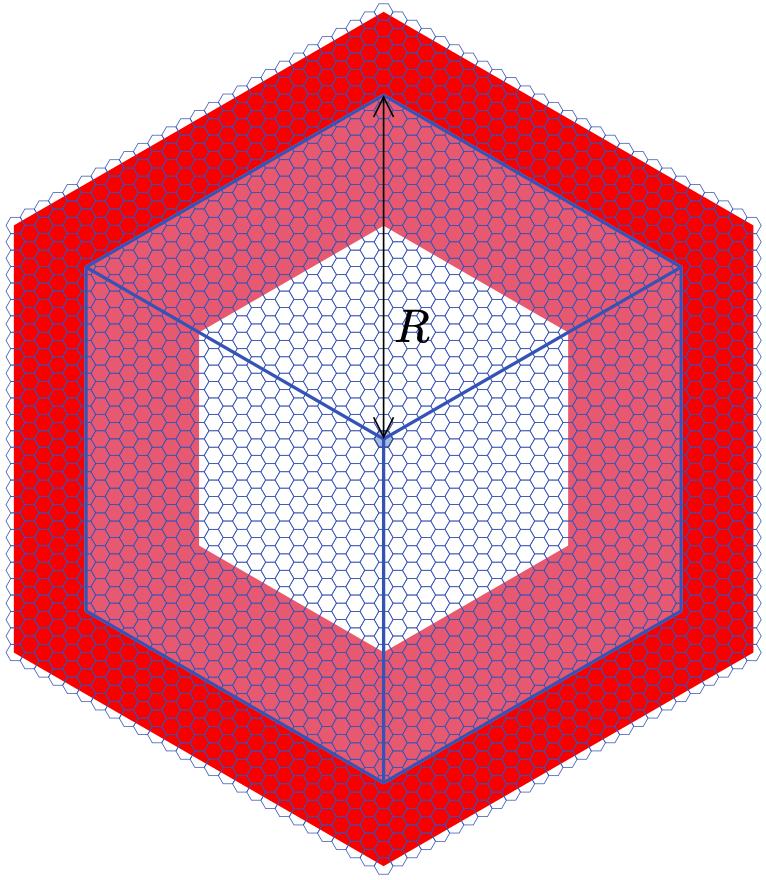
\includegraphics[width=0.5\textwidth]{images/methods/LAM_domain_zones.png}
    \caption{LAM domain structure example with NBP=27 \citep[from][]{raillard_leveraging_2024}}. The raw forcing zone is in red on the outside, the transition zone in pink, and the free zone in white at the center.
    \label{fig:LAM_domain}
\end{figure}

The concept of nudging is well known in climate modelling and NWP, since it is used to manage lateral boundary conditions in regional models. It is also used to reproduce real situations to enable the comparison to local observations with realistic synoptic conditions, or to study specific observed events with a model. 
Multiple studies were conducted using the zoom capability of LMDZ to enhance resolution over a given area, while nudging the model towards a reanalysis in the rest of the world to make sure the synoptic conditions are as close to reality as possible. In particular, land-atmosphere interactions were studied with zoomed-nudged LMDZOR simulations at the SIRTA observation site in France \citep{cheruy_combined_2013, campoy_response_2013} and over Morocco \citep{balhane_global_2022, arjdal_modeling_2024}. The main downside of this approach is that it still requires to run the model in a global simulation setup, although the grid is stretched to focus on the area of interest. With the LAM, the resolution remains the same in all the domain and the model is only run over the area of interest, which results in lower computation times than zoomed-nudged setups for a given resolution.

The model is nudged by adding a forcing term in the equation that governs the evolution of a given prognostic variable $V$ in the model, to drive it towards a reference value $V_{ref}$ over a given time scale $\tau$:

\begin{equation}
    \frac{\partial V}{\partial t} = \frac{\partial V}{\partial t}_{\text{model}}+ \frac{V_{\text{ref}} - V}{\tau}.
\end{equation}

The strength of the nudging can be modulated by adjusting the time scale $\tau$.
In the raw forcing zone, the values of the state variables in the model are directly prescribed to those of the forcing file. 
In the central free zone, $\tau$ is infinite, meaning the forcing term does not alter the equation. 
In the transition zone, the value of $\tau$ is gradually increased over the 8 grid cells, following an arctan profile to smooth the transition, starting from $\tau = 3600$ s on the outer edge.

Nudging is applied on all vertical levels at every time step of the dynamics (30 s). The reference value for each variable is obtained by temporally interpolating the forcing file to this time step. The sampling frequency of the forcing file can have an impact on the simulation. In this work, hourly forcing files were used for most of the simulations, but some sensitivity experiments were made using forcing data sampled every six hours.
%todo:compléter selon commentaire Frédérique Pas seulement le time sampling.  Tu peux peut etre mentionner la qualité du forcing. peut etre voir biblio dans les modeles regionaux

\subsubsection{Technical specificities}

While running the first simulations with the LAM, various occurrences of inappropriate model behaviour were observed at the top of the atmosphere, reaching temperatures over 373 K. Based on prior experience of the model developers, this was attributed to inconsistent quantities of air in these layers of very low density, which could lead to excessive heating over one model time step. The unusual interaction of advection from the dynamics and nudging were thought to be responsible for anomalies in the mass and energy budgets, in or near the transition zone.
To solve this issue, an additional nudging of temperature and wind components was applied for the upper layers of the atmosphere (above 1hPa) over the whole domain (including the free zone), to ensure that values remains in a reasonable order of magnitude. Given the focus on land-atmosphere interactions, this technical fix for the upper atmosphere is not considered to have any influence on the results.

It must also be noted that the model computes all variables on its hexagonal grid cells. However, analysing and displaying simulation data on such a grid is challenging because most standard tools (Ferret, ncview, Matplotlib) do not natively support its coordinate system. 
By default, LAM outputs are therefore interpolated to a regular longitude-latitude grid, but can be obtained on the native hexagonal grid if needed.
In this work, the simulations used in Chapter \ref{chap:monthly} were analysed solely using the interpolated outputs, while simulations used in Chapter \ref{chap:liaise}, which focused on specific grid cells for comparison to observation, were analysed using outputs on the native hexagonal grid.%todo:check if chapter structure has changed
%todo:Ajouter commentaires et odg sur le temps de calcul, cf simus de Frédérique : global vs LAM, nombre de tasks donc d'heures de calcul. Avantages ou non par rapport au zoomé-guidé (qui peut être forcé par ERA)

\section{ORCHIDEE land surface model}
\subsection{General structure}
ORCHIDEE (Organizing Carbon and Hydrology In Dynamic EcosystEms) is a land surface model (LSM). Various "branches" and versions exist within the model, as the base structure presented in \citet{krinner_dynamic_2005} has been adapted and extended to meet different research objectives. 
This PhD work uses branch 2.2 which is similar to the ORCHIDEE 2.0 model used in CMIP6 \citep{cheruy_improved_2020, boucher_presentation_2020} but for minor bug corrections. It also includes a global irrigation scheme that was recently developed and evaluated \citep{arboleda-obando_validation_2024}. While the version chosen for CMIP7 simulations is ORCHIDEE v4.2, which integrates recent developments for the modelling of snow, permafrost, vegetation, carbon, nitrogen and phosphorus cycles, branch 2.2 is still used for developments focused on surface hydrology, that can later be introduced in other branches.
%Coupling with an atmosphere and ocean model imposes significant computational constraints, leading to the simplification or omission of certain processes for global climate simulations.
The following description of this model version is partly based on two PhD theses \citep{campoy_influence_2013,arboleda-obando_feedback_2023}.

ORCHIDEE v2.2 includes several modules:
\begin{itemize}
    \item SECHIBA \citep[\textit{Schématisation des Échanges Hydriques à l’Interface entre la Biosphère et l’Atmo\-sphère}][]{ducoudre_sechiba_1993}. Initially developed as the surface scheme of the LMDZ GCM, this module computes surface energy and water budgets, including interactions with the atmosphere. As detailed in section \ref{sec:water}, it models water vertical infiltration and redistribution into the soil, as well as horizontal transfers through the river network.
    \item STOMATE \citep{krinner_dynamic_2005}. This module simulates biological surface processes such as photosynthesis and phenology evolution, enabling the representation of seasonal variations in leaf area index (LAI), and thus evapotranspiration.
    \item LPJ \citep{sitch_evaluation_2003}. This optional module describes the long-term evolution of vegetation to represent land use adaptation to climate and is not capable of representing fast evolutions of land use induced by human activities. Therefore, in this work, this module is inactive, and vegetation evolution is instead prescribed using annual land-cover maps described in Section \ref{sec:ORCH_input_data}.
\end{itemize}

\subsection{Atmospheric forcing}
ORCHIDEE can interface with the atmosphere in either offline mode (also called forced) or coupled mode. The simulation domain is discretized into grid cells, with a resolution that adapts to the atmospheric forcing or to the grid of the coupled atmospheric model.
In the first case, a meteorological forcing (typically obtained from a bias-corrected reanalysis) provides values for downward radiation (shortwave and longwave), precipitation (rain and snow), air temperature and specific humidity at 2 m, wind speed at 10 m (eastward and northward components), and surface pressure. 
In the second case, ORCHIDEE is coupled with an atmospheric model that calculates these variables in real time while receiving certain variables computed by ORCHIDEE (surface roughness, albedo, turbulent fluxes, surface temperature). ORCHIDEE's time step also adapts to the forcing, using 30 minutes when forced, and the same as the atmospheric physics when coupled (15 minutes for LMDZ).
Within the IPSL climate model, ORCHIDEE can be coupled with the atmospheric model ICOLMDZ in a standard configuration called ICOLMDZOR, using a semi-implicit coupling scheme \citep{polcher_proposal_1998, Hourdin_phdthesis, hourdin_2002}. This scheme calculates the vertical transfer of heat by two distinct processes: thermal diffusion in the soil and turbulent diffusion in the atmospheric column. It uses zero-flux boundary conditions at the top of the atmosphere and at the bottom of a 18-meter soil column \citep{dufresne2009description}, assuming no energy is transferred to the system at these interfaces.

\subsection{Input data}
\label{sec:ORCH_input_data}
In addition to meteorological variables, the LSM requires input data that describe the continental surface. 

Each grid cell must be assigned a soil texture which determines various hydrological and thermal soil parameters. 
For CMIP6 simulations, the map from \citet{zobler87802world} was used to assign the dominant texture in each grid cell, with a resolution of 1°. For the coupled simulations described in this work, the dominant USDA texture was obtained from the map of \citet{reynolds_estimating_2000}, which has a resolution of 5 arcmin and distinguishes 12 soil textures.

To characterize vegetation, ORCHIDEE v2.2 defines 15 Plant Functional Types (PFTs), each associated with a set of characteristic parameters used to compute their average height, leaf area index (LAI), and albedo. 
The fraction of each PFT in a grid cell is obtained from annual input maps derived from the Medium Resolution (300\,m) Land Cover product from the Climate Change Initiative (CCI) of the European Space Agency (ESA) \citep{bontemps_multi-year_2015}, and the Land Use Harmonization dataset \citep[LUH, ][]{hurtt_harmonization_2020} with the method described in \citet{lurton_implementation_2020}.
The offline simulations of Chapter \ref{chap:routing} use 0.25° resolution maps, whereas the coupled simulations in Chapter \ref{chap:monthly} and \ref{chap:liaise} use 0.1° resolution input maps. These maps change annually until 2014 and the PFT map was frozen to 2014 for the rest of the simulations (2015-2022).
For future climate simulations presented in \ref{sec:climate_change} the PFT maps were extended following the SSP5-8.5 scenario.

Each grid cell is divided into three tiles with distinct soil columns for subsurface hydrology, grouping multiple PFTs: one for bare soil, one for trees, and one for low vegetation (crops and grasses), as shown in Fig. \ref{fig:ORC_discretization} and \ref{fig:water_balance_AD}. 
Although they share the same soil texture within a grid cell, these columns were 
defined with independent water budgets to avoid large trees from extracting unrealistic amounts of moisture from the soil at the expense of the lower vegetation \citep{de1999representation}. Each PFT can influence evapotranspiration but also water infiltration into the soil through its root density.
%There is also a fraction of the soil called "nobio", dedicated to surfaces with such as ice, free water in lakes, cities \citep{ducharne_hydrol_nodate}.

\begin{figure}[hbtp]
    \centering
    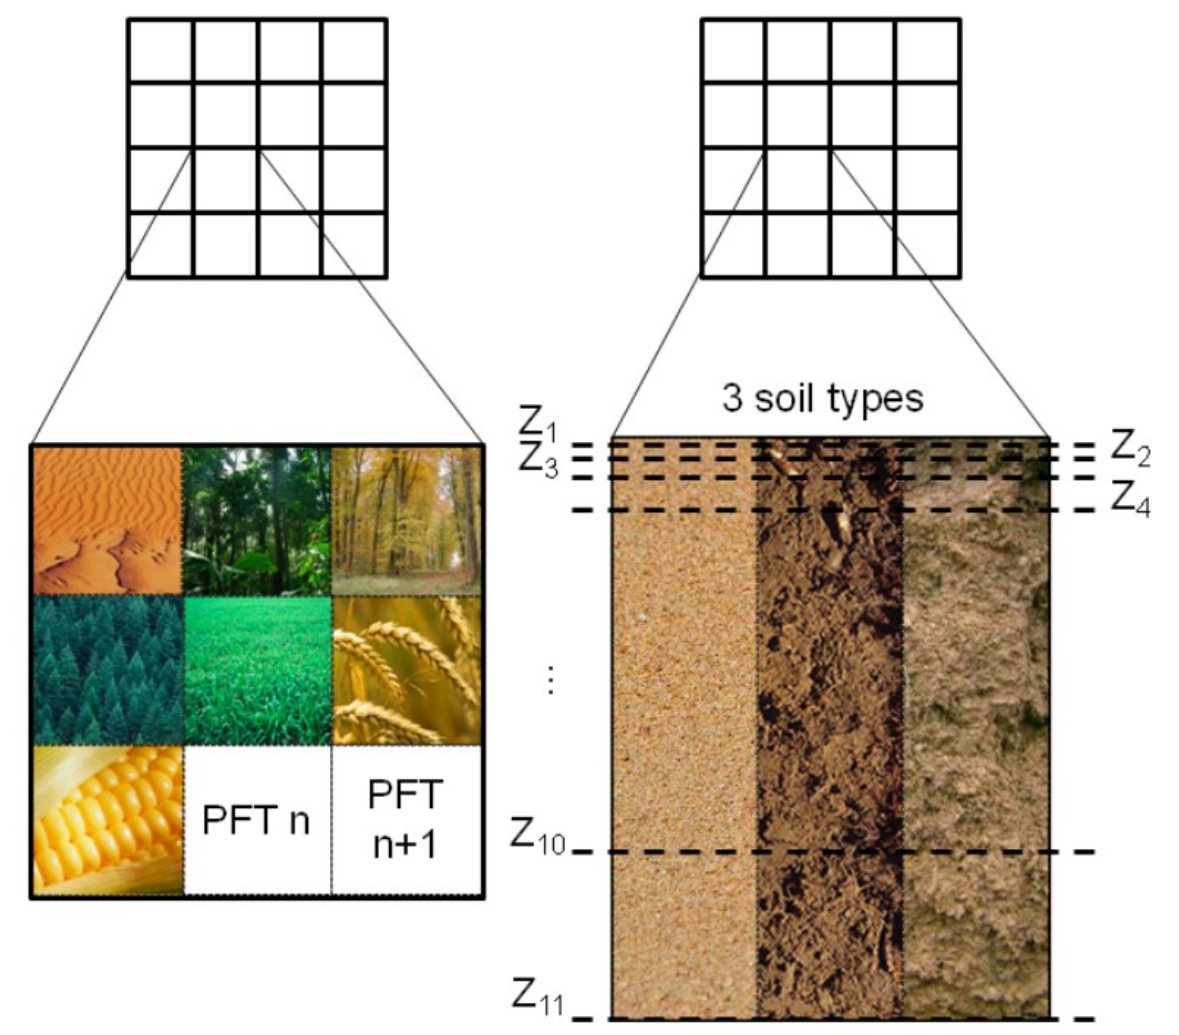
\includegraphics[width=0.5\textwidth]{images/methods/ORC_discretization.png}
    \caption{Visualisation of the ORCHIDEE PFTs and vertical discretization within one grid cell, (\href{https://orchidee.ipsl.fr/introduction/}{ORCHIDEE online documentation}).}
    \label{fig:ORC_discretization}
\end{figure}

\subsection{Water and energy budgets}\label{sec:water}

This section describes how the different terms of the water and energy budgets identified in the introduction are computed by ORCHIDEE, within the SECHIBA module. 

\subsubsection*{Precipitation partitioning}

To determine the soil water content in each soil tile of a grid cell, ORCHIDEE first separates the fraction of precipitation intercepted by vegetation and the fraction that actually reaches the ground. 
For liquid water that reaches the surface (either from rain or melted snow), it further discriminates between the portion that infiltrates into the soil and surface runoff, which occurs when infiltration is limited by hydraulic conductivity. Soil hydrology fluxes are based on the one-dimensional Richards equation, with a 2-meter soil column discretized over 11 vertical layers of increasing thickness \citep{de_rosnay_impact_2002, dorgeval_sensitivity_2008}, as shown in Fig. \ref{fig:ORC_discretization}. A free drainage condition is applied at the bottom of the column. ORCHIDEE models the infiltration front velocity, which progressively saturates the layers. The values of hydraulic conductivity and diffusivity are computed based on soil texture according to \citet{mualem_new_1976, van_genuchten_closed-form_1980}. As shown in Fig. \ref{fig:water_balance_AD}, the surface runoff and drainage computed in each grid cell then serve as input to the routing scheme, later described in Section \ref{section:routing_methods}.

Snow is represented with three layers of varying density and thermal conductivity \citep{wang_evaluation_2013}. The energy budget of the snowpack is computed, and when a layer's simulated temperature exceeds freezing, it is automatically reset to 0°C in the snow, and the excess energy is used to melt snow. The resulting liquid water may then percolate through the snowpack or be refrozen. If it reaches the soil surface, it is integrated into the surface water budget, contributing to infiltration and runoff in the same manner as rainwater.

\begin{figure}[hbtp]
    \centering
    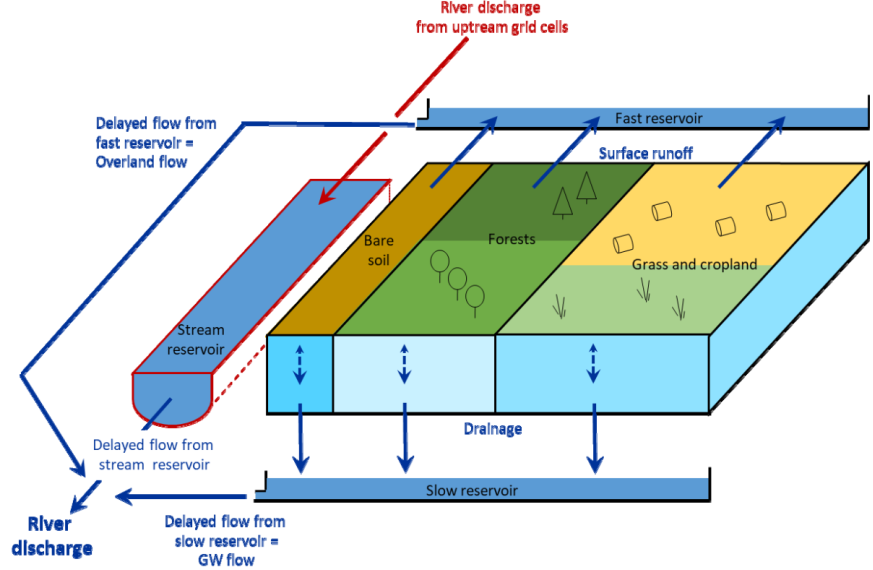
\includegraphics[width=0.8\textwidth]{images/methods/water_balance_AD.png}
    \caption{Visualisation of surface hydrology within an ORCHIDEE grid cell. (source: A. Ducharne, \href{https://forge.ipsl.fr/orchidee/attachment/wiki/GroupActivities/Training/cours_orchidee_feb2024_ducharne.pdf}{ORCHIDEE training}).}
    \label{fig:water_balance_AD}
\end{figure}


\subsubsection*{Potential and actual evapotranspiration}

The missing term to close the surface water balance is evapotranspiration $E$, which also appears in the energy balance via the latent heat flux $\lambda E$. The total evaporation value depends on potential evaporation, which represents the evaporation that would occur without water stress and thus serves as an upper limit. It is calculated using the formulation of \citet{Budyko_1956}:  

\begin{equation}
    E_{pot} = \rho_{air}  \lVert \vec{V} \rVert C_{drag, m} (q_{sat}(T_S) - q_{air})
\end{equation}

where $\rho_{air}$ is the air density, $\lVert \vec{V} \rVert$ is the horizontal wind speed, $C_{drag, m}$ is the surface drag coefficient for momentum (detailed description below), $q_{air}$ is the specific humidity of the air and $q_{sat}(T_S)$ is the specific humidity of saturated air at the surface temperature $T_S$. Air temperature, humidity, and wind speed are taken at the first level of the atmospheric model in coupled simulations, or at the height of the atmospheric forcing in offline simulations.

To obtain the actual evapotranspiration $E$ from the maximum theoretical value $E_{pot}$, ORCHIDEE computes the ratio of actual evapotranspiration to potential evapotranspiration $\beta = \frac{E}{E_{pot}}$, accounting for the four components of evapotranspiration:  

\begin{itemize}
    \item Bare soil evaporation, which is limited by the maximum volume that can be extracted from the soil column by upward water diffusion across one time step.
    %which is the minimum between $E_{pot}^*$, the potential evaporation reduced according to \citet{milly_potential_1992} and $Q_{up}$, the maximum volume that can be extracted from the soil column.
    %option:Tu peux preciser pourquoi on a besoin de Milly - Le sol n est pas une surface d'eau. Comment on evalue Q\_up - peut etre trop detaillé? 
    \item Vegetation transpiration, which is limited by the stomatal resistance of vegetation and a so-called architectural resistance which depends on vegetation structure.
    \item Evaporation of water intercepted by vegetation, which is also limited by the architectural resistance.
    \item Snow sublimation, which only concerns the regions and seasons where snowfall occurs.
\end{itemize}

To take into account these various limitations and the aerodynamic resistance which affects these four components of ET ($\frac{1}{\lVert \vec{V} \rVert C_{drag, m}}$), a conductance is identified for each component, and $\beta$ is computed as an effective conductance taking into account the fractions of the grid cell occupied by bare soil, vegetation and snow:

\begin{equation}
    \beta = f_{bare} \times \beta_{bare} + f_{veget} \times ( \beta_{transpiration} + \beta_{interception} ) + f_{snow} \times  \beta_{sublimation}
\end{equation}

It is important to note that although soil moisture might be different in each soil tile, $T_s$ (surface temperature), $C_{drag}$, and $\beta$ are computed for the whole grid cell. This means that there is a single $E_{pot}$ and evapotranspiration value for the grid cell, and therefore a single latent heat flux value.
This approach is often referred to as a composite approach, as opposed to a mosaic approach where independent fluxes are computed for each soil tile, before averaging them for coupling to the atmospheric model. 
%option: more details, limitations when comparing to obs (not able to obtain LE for a specific soiltile or PFT...), reference to Alice ?

% Bare soil evaporation is expressed as a relationship between supply and demand:
% \begin{equation}
%     E_g = min(E^*_{pot}, Q_{up})
% \end{equation}
% where $Q_{up}$ is the maximum volume that can be extracted from the soil column, and $E^*_{pot}$ is the reduced potential evaporation from \citet{Milly_1992}. Note that in most cases, $E^*_{pot} < E_{pot}$.
%NB Provide more details on the calculation of Qup? The available water volume is estimated by integrating Richards' equation over the soil column to maintain a water volume in each layer above......

% \hfill

% An alternative version exists in ORCHIDEE, which allows limiting the demand by modelling a bare soil resistance to evaporation $r_{soil}$ based on \citet{Sellers_1992}:
% \begin{equation}
%     E_g = min(\frac{E^*_{pot}}{1+\frac{r_{soil}}{r_a}}, Q_{up})
% \end{equation}
% \begin{equation}
%     r_{soil} = exp(8.206 - 4.255 \frac{W_L}{W_L^s})
% \end{equation}
% where $W_L$ is the moisture content in the top four layers of the soil column, and $W_L^s$ is the saturation moisture content in these same layers.

\hfill

\subsubsection*{Drag coefficients and roughness lengths}

There are two surface drag coefficients in ORCHIDEE, $C_{drag, m}$ for momentum and water vapour transfers, and $C_{drag, h}$ for heat transfers.
They can be computed for every PFT and depend on two roughness lengths: $z_{0m}$, below which wind speed is assumed to be zero, and $z_{0h}$, below which air temperature is assumed to be equal to the surface soil temperature. 
The default parametrization of roughness lengths in ORCHIDEE 2.2, used in this thesis, is based on \citet{su_evaluation_2001} and calculates them both dynamically, using empirical formulations which depend on the LAI. 
% However, some of the obtained values are not always consistent (particularly for $z_{0h}$), and another parametrization was introduced in ORCHIDEE, which will serve as default for CMIP7.
% With this simpler approach, the two roughness lengths depend on the canopy height of each PFT: 
% \begin{itemize}
%     \item The ratio between $z_{0m}$ and the canopy height, with a typical value of $\frac{z_{0m}}{h} = \frac{1}{15}$.
%     \item The ratio between $z_{0h}$ and $z_{0m}$, with a typical value of $\frac{z_{0h}}{z_{0m}} = \frac{1}{10}$.  
% \end{itemize}

Both drag coefficients car be expressed using a drag coefficient in neutral conditions and a stability function $f_H$:
\begin{align}
    &C_{drag,m} = C_{drag,m,neutral} f_H(Ri, z_{0m})\\
    &C_{drag,h} = C_{drag,h,neutral} f_H(Ri, z_{0m})
\end{align}

The coefficients for neutral conditions are calculated by taking into account the roughness lengths of all PFTs:
\begin{align}
    &C_{drag,m,neutral} = \sum_{i=1}^{N_\mathsf{PFT}} f_{veg,\max,i} \left[ \frac{k^2}{\left(\ln\left(\frac{z-d_{0,i}}{z_{0m,i}}\right)\right)^2} \right]\\
    &C_{drag,h,neutral} = \sum_{i=1}^{N_\mathsf{PFT}} f_{veg,\max,i} \left[ \frac{k^2}{\ln\left(\frac{z-d_{0,i}}{z_{0m,i}}\right)\ln\left(\frac{z-d_{0,i}}{z_{0h,i}}\right)} \right]
\end{align}
where ${d_{0,PFT}}$ is the displacement height, assumed equal to two thirds of the canopy height, ${k}$ is von Karman's constant and $z$ is the altitude of the atmospheric forcing.

The stability function depends on the Richardson number $Ri$, defined as the ratio of the two source terms for turbulent kinetic energy: buoyancy and wind shear, which depend on the gradient of temperature near the surface and on the surface wind speed. 
\begin{equation}
Ri= \frac{g}{\overline \theta} \frac{\frac{\partial \overline \theta}{\partial z}}{(\frac{\partial \overline u}{ \partial z})^2}
\end{equation}
A negative $Ri$ corresponds to an unstable atmosphere while positive values correspond to a stable one, and $Ri=0$ is the neutral case.
The stability function is defined differently for the unstable and stable cases, with two formulations from \citet{louis_short_1982}, which both converge towards $f_H(0)=1$.

\begin{equation}
f_H(Ri) = 
\begin{cases}
1 - \dfrac{3 B Ri}{1 + 3 B C C_{d,m,neutral} \sqrt{|Ri| \dfrac{z}{z_{0m}}}} & \text{if } Ri < 0 \\
\\
1 & \text{if } Ri=0\\
\dfrac{1}{1 + 3 B Ri \sqrt{1 + D |Ri|}} & \text{if } Ri > 0
\end{cases}
\end{equation}
with $B=C=D=5$.

\hfill

It must be noted that when ORCHIDEE is used in coupled mode with the atmospheric component of the IPSL-CM, LMDZ, ORCHIDEE does not fully compute the drag coefficients.
Instead, it computes only the neutral coefficients and provides LMDZ with effective roughness lengths for the grid cell $z_{0m,eff}$ and $z_{0h,eff}$. This modelling choice derives from the composite approach mentioned above, which is based on \textit{parameter aggregation}. Other land surface models use a mosaic approach, based on\textit{flux aggregation}, and compute turbulent fluxes for each PFT before averaging them to represent the grid cell.
Effective roughness lengths can be expressed as:
\begin{equation}
    z_{0m,eff}=z \exp{\left(\frac{-k}{\sqrt{C_{drag,m,neutral}}}\right)}
     \text{ and } 
    z_{0h,eff}=z \exp{\left(\frac{-k}{\sqrt{C_{drag,h,neutral}}}\right)}
\end{equation}
LMDZ then computes the drag coefficients using values from the surface layer for the Richardson number and its own stability functions. The formulation is similar for unstable cases, but for stable cases, functions from \cite{king_sensitivity_2001} are used:

\begin{equation}
f_{H, LMDZ}(Ri) = 
\begin{cases}
1 - \dfrac{3 B Ri}{1 + 3 B C C_{d,h,neutral} \sqrt{|Ri| \dfrac{z}{z_{0m}}}} & \text{if } Ri < 0 \\
1 & \text{if } Ri=0\\
(1-Ri/C_2)^2 & \text{if } 0 < Ri < C_2/2\\
(C_3(C_2/Ri)^2 & \text{if } Ri \geq C_2/2\\
\end{cases}
\end{equation}
with $B=C=5$, $C_2 = 0.25$, $C_3 = 0.0625$.

\hfill

\subsubsection*{Energy fluxes}

ORCHIDEE does not modify the incoming radiation terms but determines the outgoing reflected radiation terms by calculating the albedo (with distinct values for infrared and for visible light).

The heat flux into the ground, surface temperature (which controls the outgoing longwave radiation) and radiative fluxes are computed with an implicit scheme which accounts for thermal diffusion in an 18-meter soil column, with a zero-flux condition at the bottom. 
The vertical discretization matches the one used for water infiltration in the first two meters, and thermal conductivity and heat capacity are parametrized as a function of soil moisture and texture \citep{wang_improvement_2016}.
When coupled to LMDZ, the aforementioned semi-implicit coupling scheme is used, which also computes turbulent diffusion is the atmospheric column at the same time as thermal diffusion in the soil \citep{polcher_proposal_1998, Hourdin_phdthesis, hourdin_2002}. 

The latent heat flux is expressed directly from the evapotranspiration, while the sensible heat flux uses a similar formulation:
\begin{equation}
    LE = \lambda \beta E_{pot} = \lambda \beta \rho_{air} \lVert \vec{V} \rVert C_{drag, m} (q_{sat}(T_S) - q_{air})
\end{equation}
\begin{equation}
    H = \rho_{air}  \lVert \vec{V} \rVert C_p C_{drag, h} (T_{surf} - T_{air})
\end{equation}
where $\rho_{air}$ is the air density, $\lVert \vec{V} \rVert$ is the horizontal wind speed, $C_p$ is the is the specific heat of air, $C_{drag, h}$ is the surface drag coefficient for heat, $T_{air}$ is the air temperature, and $T_{surf}$ is the surface temperature (sometimes referred to as the skin temperature).

\subsection{Routing scheme}
\label{section:routing_methods}
The routing scheme is a sub-module of SECHIBA, which simulates horizontal water transfers between grid cells and transports water to the oceans \citep{ducharne_development_2003, ngo-duc_validation_2007}. 
Water routing is necessary to maintain water conservation on a global scale in fully coupled simulations with a dynamic ocean model, and it also enables simulation of river discharge and groundwater volumes. 
This scheme generally runs at a larger time step than the rest of the model (once per day by default in global simulations). However, the irrigation scheme (Section \ref{sec:irrig_methods}) requires the routing to be performed at the same time step as the soil hydrology computed by SECHIBA. 

The routing scheme subdivides the simulation domain into hydrological transfer units (HTU) and uses a digital elevation model (DEM) constructed from topographic data to define flow directions and characterize the HTUs (dimensions, slope, upstream/downstream relationships). The grid of the HTUs, upon which the routing flows are solved, is often different from the ORCHIDEE grid, and is hereafter referred to as the routing grid.

Within each HTU, three linear reservoirs are represented: the \textit{slow} reservoir (groundwater), the \textit{fast} reservoir (overland water), and the \textit{stream} reservoir (rivers). For each reservoir, the characteristic residence time of water in one HTU depends on a fixed transfer coefficient (denoted TCST\_SLOW, TCST\_FAST, and TCST\_STREAM in Fig. \ref{fig:routing_principles}), on the size of the HTU and on the local slope obtained from the DEM.
Surface runoff and drainage computed for each ORCHIDEE soil column are regridded to the routing grid to respectively feed the overland and groundwater reservoirs. All three reservoirs then flow into the river reservoir of the downstream HTU. The river reservoir is therefore the only one connected to neighbouring HTUs, as no other horizontal transfer is modelled in ORCHIDEE. This assumption may have limitations at high resolutions as it ignores direct groundwater transfers between HTUs.

The outgoing water quantity $Q$ (given in $kg$) from a reservoir over one routing time step is expressed using the reservoir volume in the routing grid cell $V$ ($kg$), the transfer coefficient of the reservoir $TCST$ ($day \cdot km^{-1}$), a topographic index $topoindex$ ($km$), and the routing time step $dt_{routing}$ ($s$):

\begin{equation}
    Q = \frac{V}{topoindex \times TCST} \times \frac{dt_{routing}}{86400}
\end{equation}

The transfer coefficient reflects the roughness that creates a resistance to flow in this reservoir. The model assumes this parameter to be unique over the whole simulation domain, with a smaller value for the river reservoir than for the overland reservoir, and a larger one for the groundwater reservoir.
For a given DEM grid cell, the topographic index is defined as the length of the grid cell in the flow direction ($d$) divided by the slope ($\delta z / d$):
\begin{equation}
    topoindex = \frac{d}{\sqrt{\frac{\delta z}{d}}} = \sqrt{ \frac{d^3}{\delta z} } 
\end{equation}

Several versions of the routing scheme have been developed in ORCHIDEE, all based on these modelling principles but corresponding to different relationships between the routing grid and the ORCHIDEE grid:

\begin{itemize}
\item \textbf{\textit{Subgrid\_halfdeg} routing}, which was the default option in branch 2.2 until CMIP6. It is designed to work with a specific DEM at a resolution of 0.5°.
Depending on the resolution of the ORCHIDEE grid, a given (whole) number of HTUs are defined within each ORCHIDEE grid cell. Since there are a whole number of HTUs in each ORCHIDEE grid cell, the regridding of surface runoff and drainage to the routing grid is only a partitioning using the areal fraction covered by each HTU.
Based on the DEM, a $topoindex$ value and slope direction are defined for each HTU using preprocessing scripts before starting the simulation.
In this manuscript, this routing was only used in Chapter \ref{chap:routing},  with an ORCHIDEE grid at 0.5° resolution, similar to the DEM, meaning there is always only one HTU per ORCHIDEE grid cell. 
It must be noted that this routing code is not compatible with non-regular ORCHIDEE grid cells, and can therefore not be used with the icosahedral grid of ICOLMDZOR.

\item \textbf{\textit{Subgrid\_HTU} routing}, largely based on \std, but adapted to used higher resolution DEMs \citep{nguyen-quang_orchidee-routing_2018, polcher_hydrological_2023}. However, this routing  also presents the constraint of having an integer number of HTUs within each ORCHIDEE grid cell, making it incompatible with the icosahedral grid of ICOLMDZOR. It was not used in the simulations presented in this thesis, but the manuscript occasionally refers to it.

\item \textbf{\textit{Interp\_topo} routing}, recently implemented by Yann Meurdesoif in ORCHIDEE to become the default version in IPSL-CM7. 
It is designed to adapt to any DEM resolution and to be completely independent of ORCHIDEE’s resolution and even of the shape of the grid cells. This is particularly necessary for compatibility with the icosahedral grid of the new atmospheric dynamics (DYNAMICO) of IPSL-CM7.
In this version, the routing grid is exactly the same as the DEM grid, meaning that the HTUs are exactly the DEM grid cells. This scheme relies on a robust interpolation \citep{kritsikis_conservative_2017} of runoff and drainage from the ORCHIDEE grid to the routing grid, where horizontal transfers between reservoirs are performed. Once these transfers are completed, water volumes in the reservoirs are re-interpolated from the routing grid back to the ORCHIDEE grid, allowing them to be used for irrigation within ORCHIDEE grid cells. 
A simplified calibration experiment had been carried out over the Danube basin \citep{kilic_evaluation_2023} but this PhD thesis provides the first evaluation and use case of this new routing in both offline and coupled simulations (Chapters \ref{chap:routing} and \ref{chap:monthly}).
Its principles are presented in Fig.\ref{fig:routing_principles}.
\end{itemize}


\begin{figure}[ht]
    \centering
    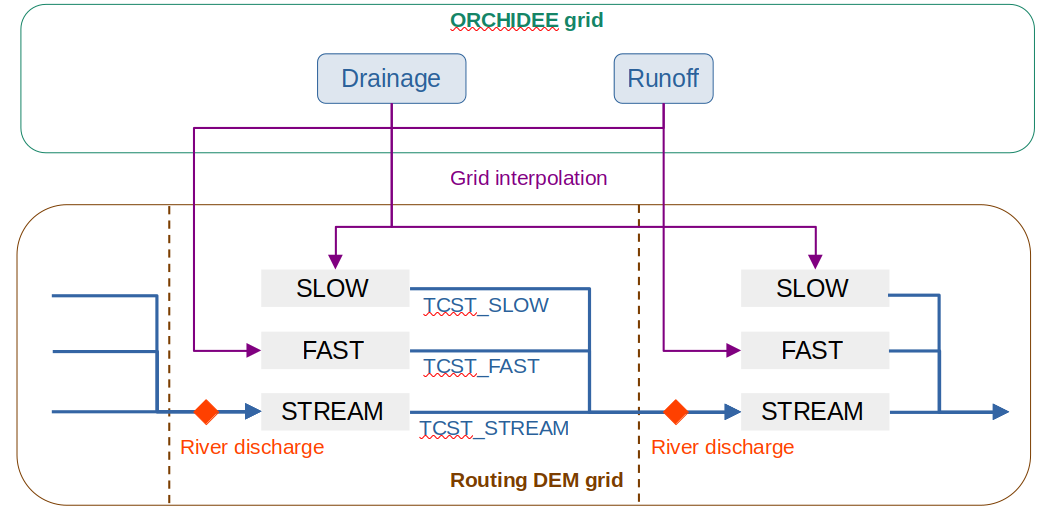
\includegraphics[width=1\textwidth]{images/methods/routing_principles.png}
    \caption{Modelling principles of the \textit{interp\_topo} routing.}
    \label{fig:routing_principles}
\end{figure}

Two DEMs are used in this work, with different resolutions. 
The first one is the 0.5° resolution DEM that has long been used within ORCHIDEE with the \std routing, based on the topography and flow directions of \citet{vorosmarty_geomorphometric_2000}.
The second one is a 1-arcminute ($\approx$ 2 km) resolution DEM based on the MERIT Hydro DEM \citep{yamazaki_merit_2019}.
The \std routing can only use the 0.5° DEM whereas the \native can be used with any DEM.

%option:show map of DEMs over the region -> not easy because big files on JZ but doable ?
%option:mention river discharge stations, positionning on DEM ? Or keep that for dedicated chapter ?

\subsection{Irrigation scheme}
\label{sec:irrig_methods}
\subsubsection{Modelling principles}

Irrigation has long been described in ORCHIDEE, using potential evapotranspiration as a target to define the irrigation amounts \citep{de_rosnay_integrated_2003, guimberteau_global_2012}. A new irrigation scheme was recently implemented in ORCHIDEE, presented and validated in \citet{arboleda-obando_validation_2024}. It is based on a water-conservative supply-and-demand approach, and uses a target soil moisture, more easily comparable with real irrigation practices, with more complex water allocation rules than the previous scheme. The present work relies solely on the new modelling approach, summarized in Figure \ref{fig:schema_pedro}.

\begin{figure}[t]
    \centering
    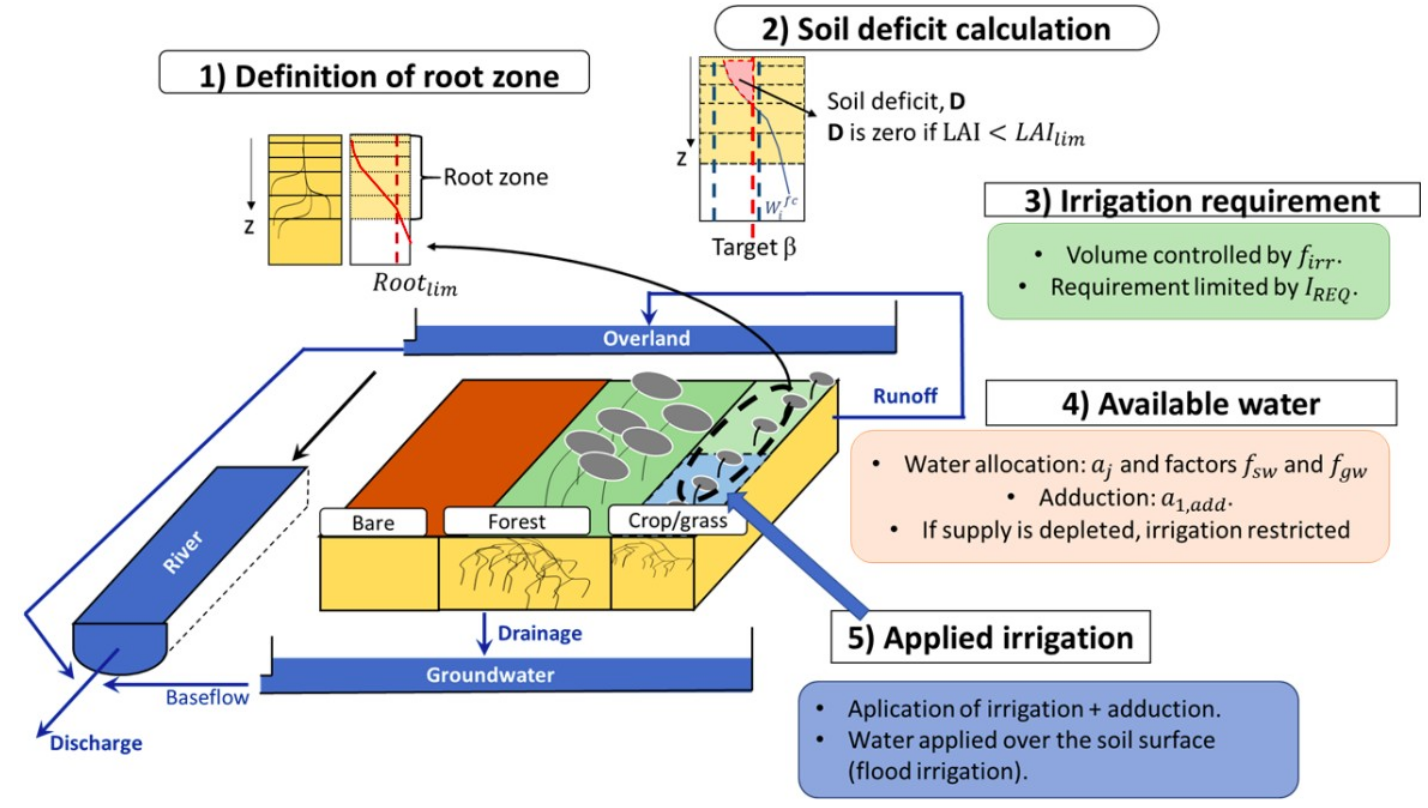
\includegraphics[width=1\textwidth]{images/methods/schema_pedro.png}
    \caption{Principles of the new irrigation scheme \citep[from][]{arboleda-obando_validation_2024}. Here, target parameter \betairrig is simply denoted $\beta$.}
    \label{fig:schema_pedro}
\end{figure}

First, an irrigated root zone is defined using parameter $z_{IRZ}$ in meters, which determines the depth of the considered root zone. In all the simulations presented here, $z_{IRZ} = 0.64$ was used, accounting for a 64-centimetre root zone. This value was selected in \citet{arboleda-obando_validation_2024} to account for 90\% of the root density in global simulations, and defined as the default parameter value. It is important to note that irrigation only applies to the column of low vegetation PFTs (grasses and crops), and the irrigated root zone is defined exclusively within this column.
A target soil moisture value is also defined, supposed to be optimal to sustain plant growth. It is expressed as a fraction of the soil moisture at field capacity water content (parameter \betairrig).

Given this target value and the soil moisture in the root zone, a soil moisture deficit $D$ (mm) is calculated as the sum of deficits across all layers of the root zone:
\begin{equation}
    D = \sum_{z_i < z_{IRZ}} min(0,\beta_{irrig} \times W_i^{fc} - W_i)
\end{equation}
where $W_i$ and $W_i^{fc}$ are respectively the soil moisture and field capacity soil moisture of layer $i$ (in mm).

In the absence of active vegetation (notably in winter), it is not relevant to compute a soil moisture deficit and an irrigation demand. A parameter $LAI_{lim}$ is therefore defined as a threshold LAI value below which the soil moisture deficit is zero. The default value is $LAI_{lim}=0.1$.

For a SECHIBA module time step $dt$ (by default 15 minutes in ICOLMDZOR simulations, 30 minutes in offline ORCHIDEE simulations), the irrigation demand hourly rate is $D/dt$ (mm/h). However, if the hourly irrigation rate is significantly higher than the infiltration rate into the soil, the model may produce excessive runoff that is not representative of reality. To prevent this, even if the moisture deficit is very high, the irrigation demand hourly rate is capped by a maximum value $I_{\max} = 3 mm \cdot h^{-1}$.

Finally, the water demand for the column is weighted by the fraction of the grid cell that is irrigated: $f_{irr}$. This fraction is obtained from the HID map at 5 arc-min resolution \citep{siebert_quantifying_2010}, and can be updated each year over the course of the simulation.
This irrigated fraction must not exceed the fraction of the soil column containing grasses and crops, as irrigation is only applied to this column.

The irrigation demand $I_{req}$ is therefore:
\begin{equation}
    I_{req} = f_{irr} \, \min(D/dt, I_{\max}).
\end{equation}

Once this demand is computed, the irrigation scheme searches for available water in the three routing reservoirs of the grid cell.
The volume of water available for irrigation is expressed as:
\begin{equation}
    A_w = f_{sw} \, (a_1 S_1 + a_2 S_2)+ f_{gw} \, a_3 S_3,
\end{equation}
where $S_i$ represents the water volume (in mm) in each of the reservoirs (rivers, overland, groundwater), and for each reservoir, a parameter $a_i \in [0;1]$ limits the total volume that can be withdrawn. This ensures that a certain amount of water remains in each reservoir, representing physical constraints and environmental regulations on irrigation withdrawals.
The fractions $f_{sw}$ and $f_{gw}$, ranging from 0 to 1, represent the accessibility of different reservoirs (surface water and groundwater, respectively) within the grid cell. These fractions are obtained from the global map of areas equipped for irrigation, from \citet{siebert_groundwater_2010}. A key feature of this map is that a given pumping point cannot be equipped for both surface water and groundwater use simultaneously, which translates to $f_{sw} + f_{gw} =1$.

Once the demand $I_{req}$ and supply $A_w$ are calculated, the applied irrigation is simply  determined as:
\begin{equation}
    I = \min(A_w/dt, I_{req}).
\end{equation}

Within the limit of $f_{sw}$ and $f_{gw}$, water is primarily withdrawn from the river reservoir, and only if this is insufficient to meet the demand are the other reservoirs tapped.
At the next time step, the amount of water withdrawn from the reservoirs, $I$, is added at the top of the ORCHIDEE soil column and infiltrates, simulating a gravity-fed or drip irrigation method.
It must be noted that although the original irrigation scheme from \citet{arboleda-obando_validation_2024} included the possibility to withdraw water from neighboring grid cells to represent adduction systems, this option is not yet compatible with the new version of the routing scheme used with ICOLMDZOR and was therefore not used in this work.

To summarize, Table \ref{tab:irrigation_parameters} gives the default value of all the parameters used by the irrigation scheme, while Fig. \ref{fig:irrig_inputs} shows the two input maps over the Iberian Peninsula: the map of irrigated fractions, to obtain $f_{irr}$, and the map of areas equipped for irrigation, to obtain $f_{sw}$ and $f_{gw}$.
The sensitivity analyses described in \citet{arboleda-obando_validation_2024} allowed the authors to define default values for all parameters to best match observed global irrigation when used uniformly, and showed that the target parameter $\beta$ has the greatest impact on the volume of water withdrawn for irrigation.
In the default version of the global model, this parameter is set to 0.9, defining a soil moisture target at 90 \% of field capacity. However, this value reflects a wide variety of irrigation practices, from drip irrigation to flooding of rice paddies, and might need to be adjusted for simulations focused on a specific region as discussed in Chapter \ref{chap:routing}.

\begin{table}[htbp]
    \centering
    \begin{tabular}{|l|p{7cm}|c|}
        \hline
        \textbf{Parameter name} & \textbf{Description} & \textbf{Default value} \\
        \hline
        $z_{IRZ}$ & Root zone depth. & 64 cm \\ %cum_dh_thr
        \hline
        \betairrig & Target soil moisture (as a percentage of soil moisture at field capacity). & 90 \% \\%beta_irrig
        \hline
        $LAI_{lim}$ & Minimum leaf area index (LAI) threshold for irrigation activation. & 0.1 \\ %lai_irrig_min
        \hline
        $I_{max}$ & Maximum allowable irrigation rate. & 3 mm $\cdot h^{-1}$ \\ %irrig_dosmax
        \hline
        $a_i$ & Fraction of reservoirs that can be withdrawn. & 90 \%  (for each reservoir)\\ %avail_reserv
        \hline
    \end{tabular}
    \caption{Parameters used in the irrigation scheme and their default values.}
    \label{tab:irrigation_parameters}
\end{table}

\begin{figure}[htbp]
    \centering
    \begin{subfigure}[b]{0.48\textwidth}
        \caption{}
        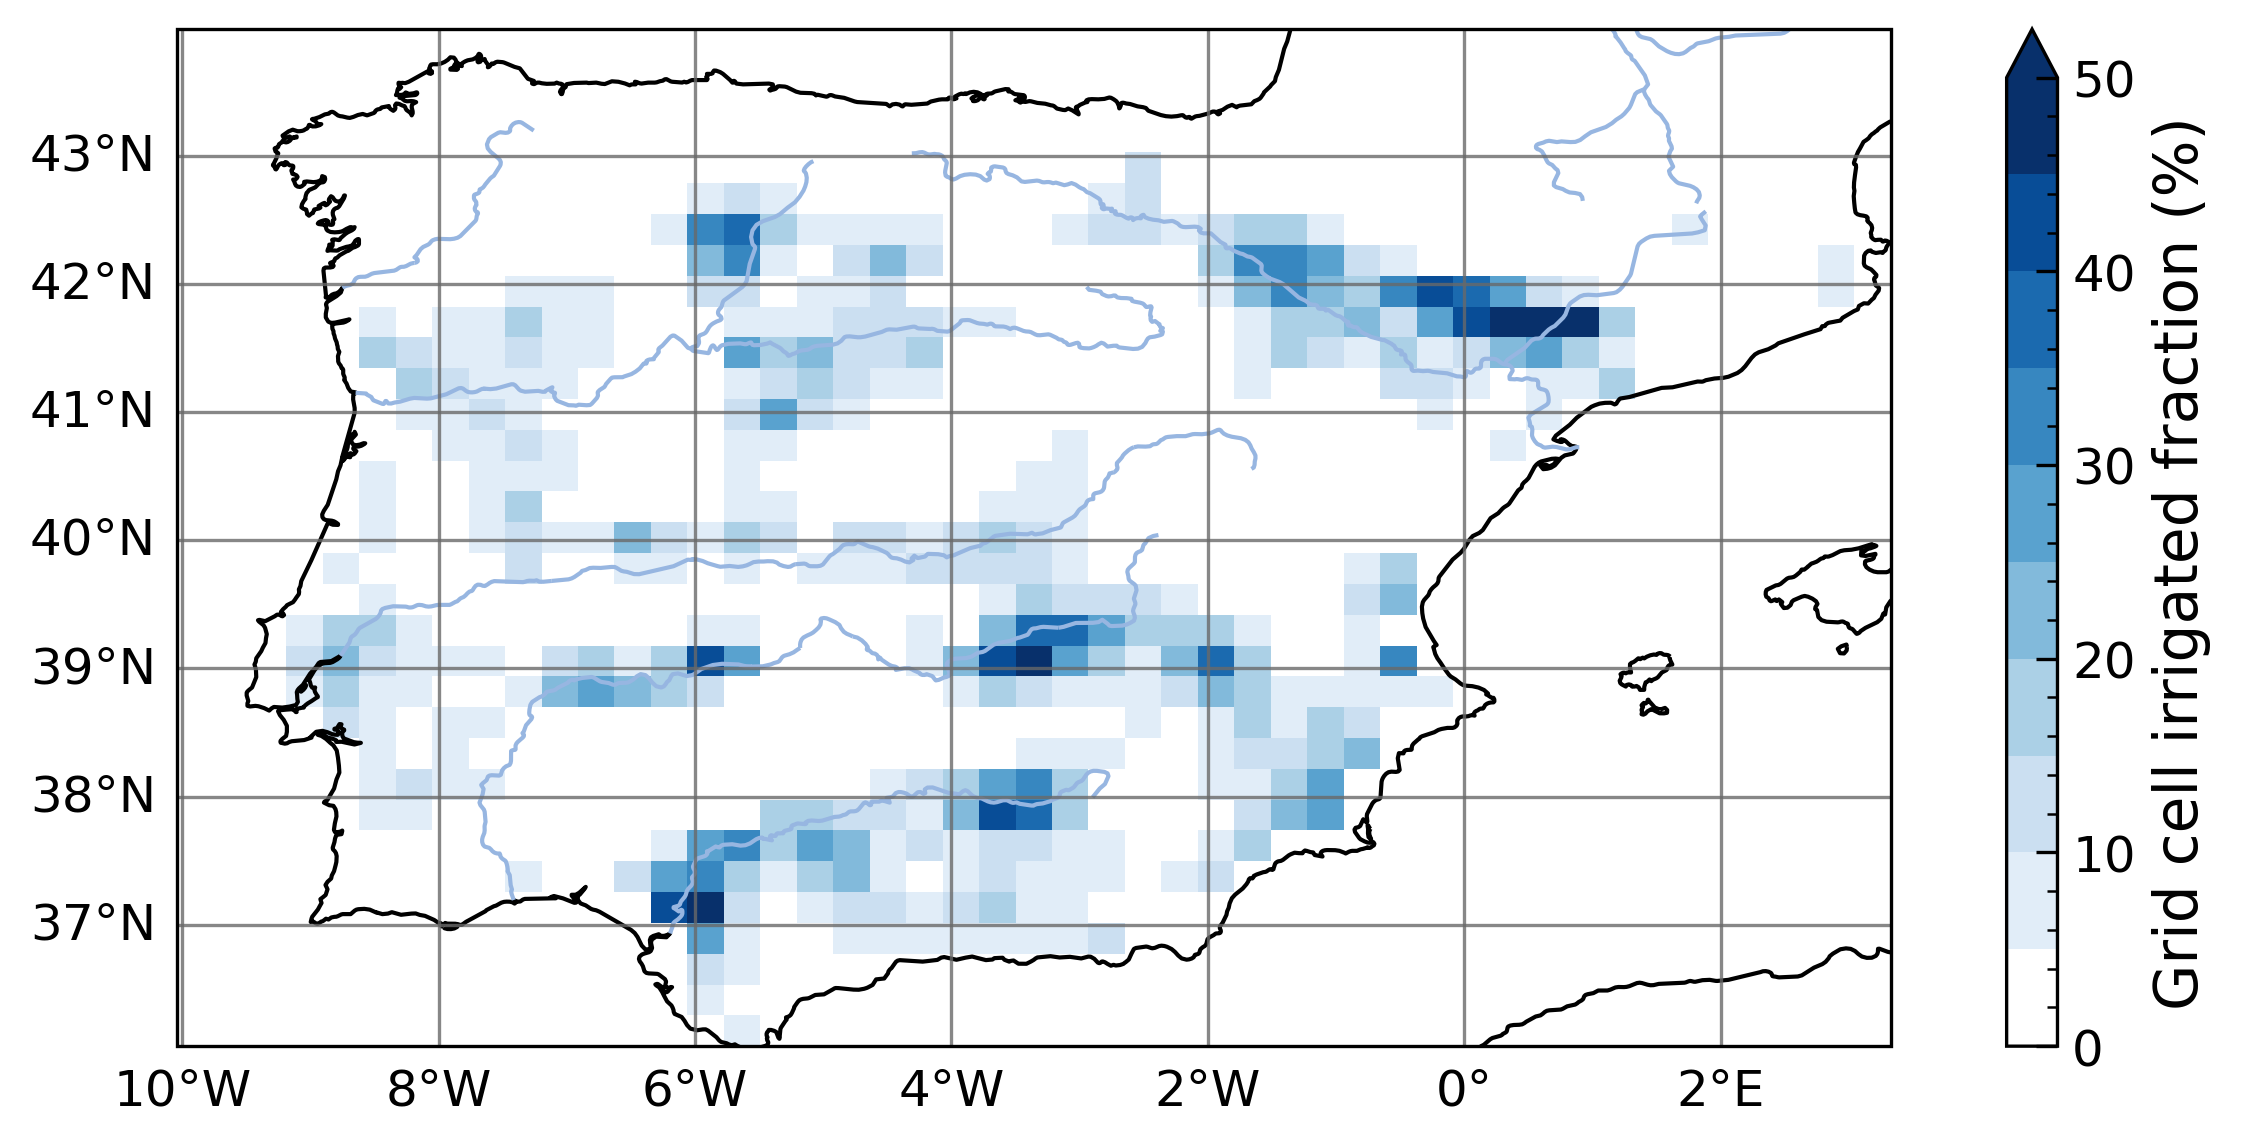
\includegraphics[width=\textwidth]{images/methods/irrigated_fraction_map.png}
    \end{subfigure}
    \begin{subfigure}[b]{0.48\textwidth}
        \caption{}
        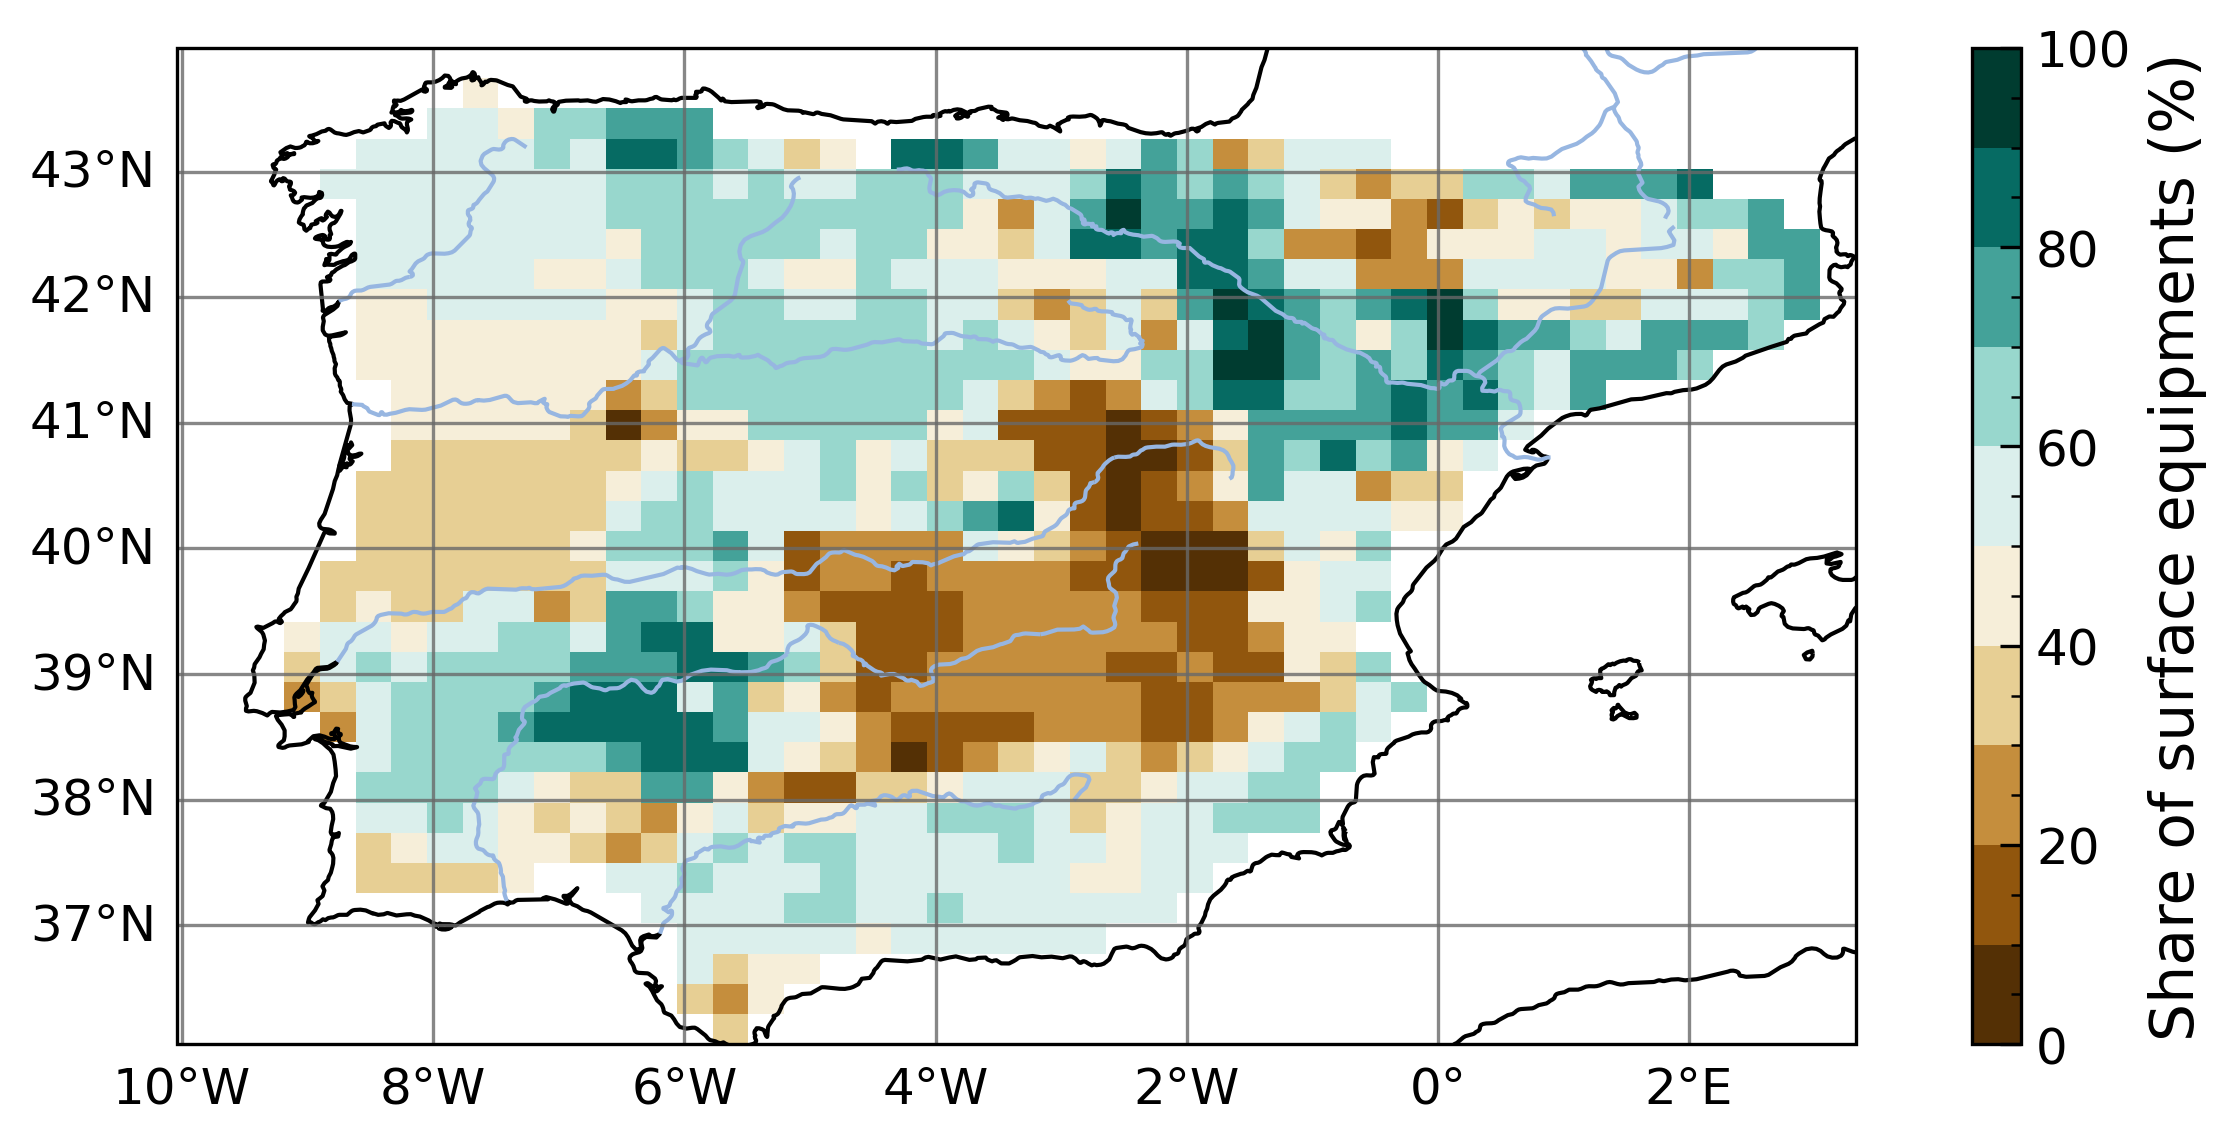
\includegraphics[width=\textwidth]{images/methods/aei_sw_map.png}
    \end{subfigure}
    \caption{Input maps of the irrigation scheme over the study area: (a) grid cell irrigated fraction \citep[\%, derived from][]{hurtt_harmonization_2020}, and (b) the share of surface equipments for irrigation withdrawals, as opposed to groundwater withdrawals \citep[\%, derived from][]{siebert_groundwater_2010}.}
    \label{fig:irrig_inputs}
\end{figure}
%todo: comment for future links : main irrigated valleys (mention coast no irrigated ?), dependency to GW or surface water (identify Ebro vs Andalousia)

\subsubsection{Irrigation scheme with the \native routing.}
\label{sec:irrig_interp_variables}

This irrigation scheme was initially developed for the \std routing version, and adjustments were made when developing the \native routing to make it compatible with this new routing code. Since the routing grid is completely independent of the ORCHIDEE grid in \native, it is important to identify which variables are computed directly on the ORCHIDEE grid and which ones are computed on the routing grid, and then interpolated to the ORCHIDEE grid to be used as ORCHIDEE outputs.
In particular, reservoir volumes are computed on the routing grid, which means that irrigation (which withdraws from these reservoirs) must be computed on the same grid.
To ensure water conservation, the \native routing uses absolute values in $kg$ of water (as opposed to areal values in $kg \cdot m^{-2}$). Therefore, when interpolating variables from one grid to another, the variables are also converted to a different unit, accounting for the continental area of the ORCHIDEE grid cells.
The only variable that is output directly on the routing grid is the river discharge, which cannot be averaged in a conservative way. Since the routing grid is of higher resolution than the ORCHIDEE grid, it also enables a more relevant comparison to discharge observation stations.
Figure \ref{fig:irrig_interpolations_outputvars} summarizes the interactions between the two grids for routing and irrigation variables in \native.

\begin{figure}[htbp]
    \centering
    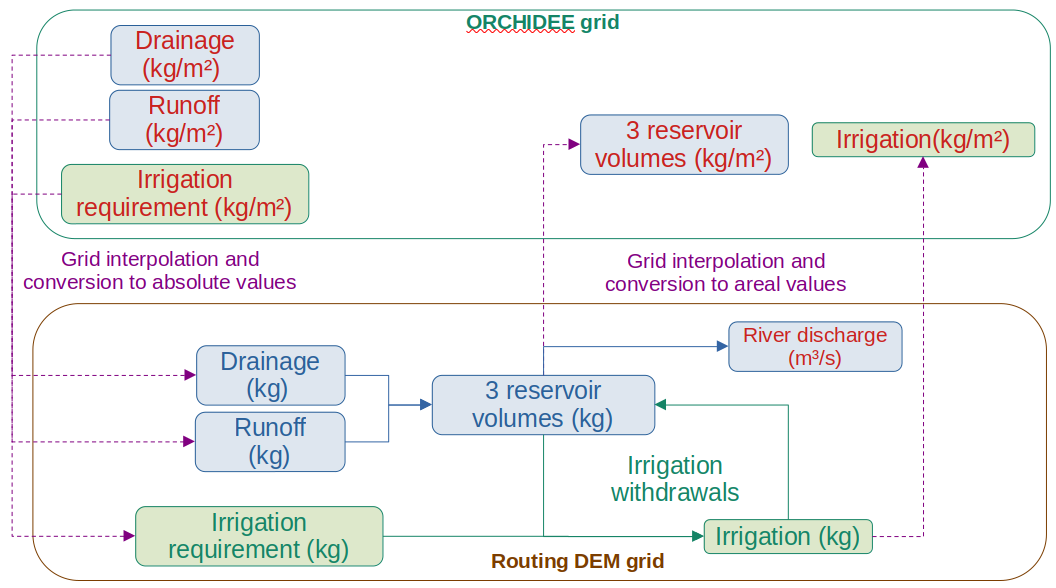
\includegraphics[width=\textwidth]{images/methods/routing_irrig_interpolation_outputvars.png}
    \caption{River routing and irrigation variables and interactions between the ORCHIDEE and routing grids in \native. Variables shown in red are used as model outputs while the others are only intermediate computations.}
    \label{fig:irrig_interpolations_outputvars}
\end{figure}

\chapter{Evaluation and parameter tuning of a new routing scheme over the Iberian Peninsula}
\label{chap:routing}
\minitoc
\pagebreak
% \chapter{Evaluation and calibration of a new routing scheme over the Iberian Peninsula}
\label{chap:routing}
\minitoc
\pagebreak

\section{Chapter introduction}

This chapter presents the preliminary work to evaluate and calibrate the new version of the routing scheme (\native) before running coupled simulations with ICOLMDZOR. As a reminder, the pre-existing version of the routing scheme, \std, cannot be used with ICOLMDZOR because it imposes constraints on the ORCHIDEE and routing grids that are incompatible with the icosahedral grid. 
The \native routing is based on the same modelling principles (described in Chapter \ref{chap:methods}) as \std but relies on a new code to interpolate between the ORCHIDEE grid and the routing grid, and other changes to make it compatible with any DEM and ORCHIDEE grid.

Two objectives were initially identified:
\begin{itemize}
    \item Ensure that the \native code could replicate the general behaviour and order of magnitudes of \std if given the same parameters and DEM as input. 
    \item Evaluate and calibrate \native using a high resolution DEM over the Iberian Peninsula to identify an appropriate set of parameters for coupled simulations.
\end{itemize}

However, this work raised more general scientific questions, which were addressed using offline simulations with different experimental setups. The routing modelling principles are theoretically independent of the spatial and temporal resolution but using \native allowed to look into the effects of changing to a high resolution DEM. During the calibration, which used discharge observations as a reference, the relative importance of various factors was also analysed, such as the meteorological forcing used and the activation of irrigation. It also raised the question of how the irrigation scheme could be adapted to better match regional practices and achieve more realistic values of river discharge in irrigated river basins. Finally, an important question was the impact and strength of the interdependency between irrigation, the water volume in the river reservoir and simulated river discharge in large basins.

\section{Methods for the routing scheme evaluation and calibration}

The relevant routing outputs for evaluation and calibration are river discharge and water volumes in each of the reservoirs (groundwater, overland, rivers). 
It must be noted that these volumes cannot be easily compared to observations, since large-scale measurements of groundwater or river volumes are complex and may not physically correspond to the abstraction level of the reservoirs modelled in ORCHIDEE.
Their importance in this work is mainly justified by the fact that the irrigation scheme withdraws water from these reservoirs to satisfy the irrigation demand while conserving water.

All simulations for this chapter were run in offline mode, meaning that ORCHIDEE is not coupled to any atmospheric model but takes meteorological data as input. 
Most simulations were run from 2000 to 2012, with the WATCH Forcing Data ERA-Interim \citep[WFDEI, ][]{weedon_wfdei_2014}. Sensitivity experiments to assess the impact of the forcing were also run with the Global Soil Wetness Project Phase 3 Atmospheric Boundary Conditions \citep[GSWP3, ][]{kim_hyungjun_global_2017}, another forcing dataset which is only available until 2010.
In all simulations, the first three years were considered as a spin-up and removed from the analysis, to allow the vegetation and hydrological variables to reach an equilibrium. The regional domain covers the Iberian Peninsula and part of Morocco, since at the time, this region was also considered as a study area for coupled simulations. Since this idea was not pursued, the analysis only focuses on the Iberian Peninsula.
Topographical data from the two DEMs presented in Chapter \ref{chap:methods} was used, either from the 0.5°-resolution DEM historically associated with the \std routing or from the MERIT DEM at 2-km resolution.

In all this chapter, the simulated river discharge is evaluated against monthly observation data from discharge stations of the Global Runoff Data Center \cite[GRDC, https://grdc.bafg.de,][]{fekete_global_2003}.
Stations were positioned on the 0.5° DEM grid using only the GPS position, and on the MERIT DEM grid with tools presented in \cite{polcher_hydrological_2023}, which use the GPS position of the stations as well as the upstream catchment area to find the most appropriate grid cell for comparison with the observations. 
Four stations were used, which are all on large rivers (Ebro, Douro, Tagus, Guadiana) and show large discharge values, meaning they represent the integrated discharge over a large share of the basins.

\begin{figure}[htbp]
    \centering
    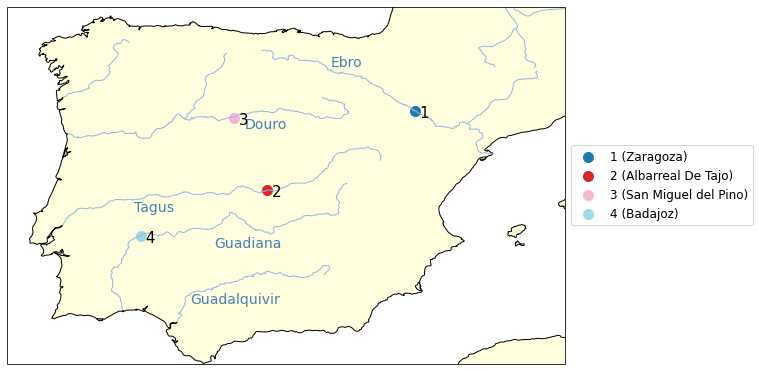
\includegraphics[width=0.7\textwidth]{images/chap3/river_discharge/halfdeg_4stations_map.png}
    \caption{Discharge stations selected for the routing scheme evaluation and calibration.}
    \label{fig:halfedg_stations_map}
\end{figure}

\section{Consistency of \native with \std routing}
\subsection{Simulation experiments}

This first analysis used the \native routing in the same setup as the \std routing. 
The input DEM was the same (0.5° resolution), and the time constants for the three reservoirs were the same as the default values for the global model (Table \ref{table:tcst_consistency}).
Four simulations were run, two without irrigation (labeled as \textit{no\_irr}) to assess the routing schemes without its influence, and two with irrigation (labeled as \textit{irr}). It must be noted that these simulations were not aimed at evaluating the realism of simulated irrigation or discharge (which will be addressed in Section \ref{section:calib}) but only to assess if the new routing code behaves similarly to the previous version.

\begin{table}[h]
\centering
\begin{tabular}{|c|c|c|}
\hline
\textbf{TCST\_SLOW} & \textbf{TCST\_FAST} & \textbf{TCST\_STREAM} \\ \hline
25            & 3             & 0.24            \\ \hline
\end{tabular}
\caption{Routing time constant for the consistency analysis ($day \cdot km^{-1}$).}
\label{table:tcst_consistency}
\end{table}

\subsection{Differences between \native and \std on coastal grid cells}

%figure : 12 maps of mean reservoir volumes and hydrographs, for both sims and diff
\begin{figure}[htbp]
    \centering
    \begin{tabular}{ccc}
        \begin{subfigure}[b]{0.33\textwidth}
            \caption{Groundwater reservoir\\(annual mean, \std)}
            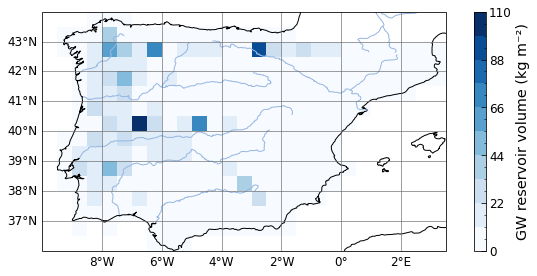
\includegraphics[width=\textwidth]{images/chap3/maps/slowr_subgrid.png}
        \end{subfigure} &
        \begin{subfigure}[b]{0.33\textwidth}
            \caption{Groundwater reservoir\\(annual mean, \native)}
            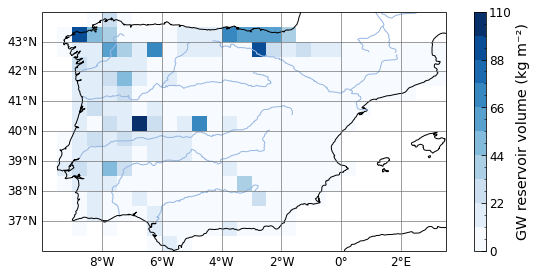
\includegraphics[width=\textwidth]{images/chap3/maps/slowr_interp.png}
        \end{subfigure} &
        \begin{subfigure}[b]{0.33\textwidth}
            \caption{Groundwater reservoir difference (\native -\std)}
            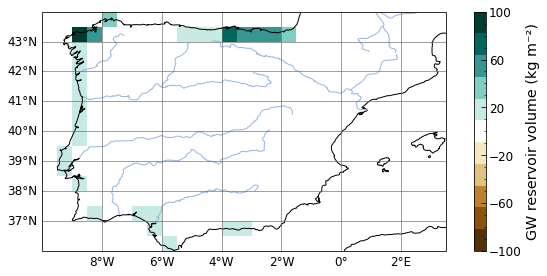
\includegraphics[width=\textwidth]{images/chap3/maps/slowr_diff.png}
        \end{subfigure} \\
        
        \begin{subfigure}[b]{0.33\textwidth}
            \caption{Overland reservoir\\(annual mean, \std)}
            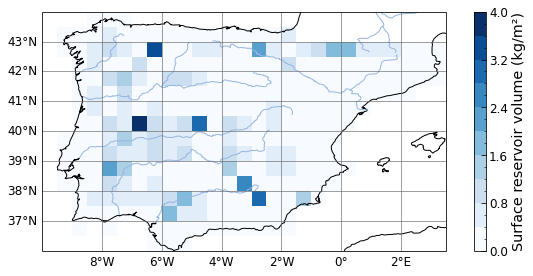
\includegraphics[width=\textwidth]{images/chap3/maps/fastr_subgrid.png}
        \end{subfigure} &
        \begin{subfigure}[b]{0.33\textwidth}
            \caption{Overland reservoir\\(annual mean, \native)}
            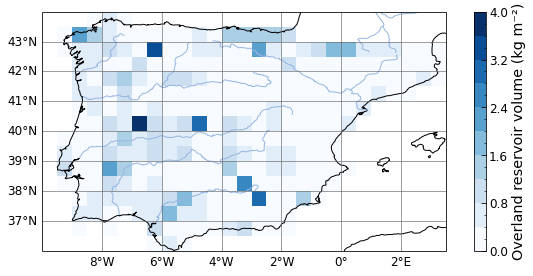
\includegraphics[width=\textwidth]{images/chap3/maps/fastr_interp.png}
        \end{subfigure} &
        \begin{subfigure}[b]{0.33\textwidth}
            \caption{Overland reservoir difference (\native -\std)}
            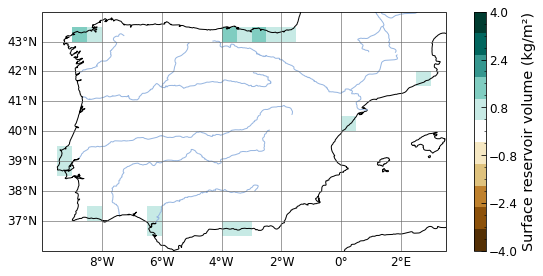
\includegraphics[width=\textwidth]{images/chap3/maps/fastr_diff.png}
        \end{subfigure} \\
        
        \begin{subfigure}[b]{0.33\textwidth}
            \caption{River reservoir\\(annual mean, \std)}
            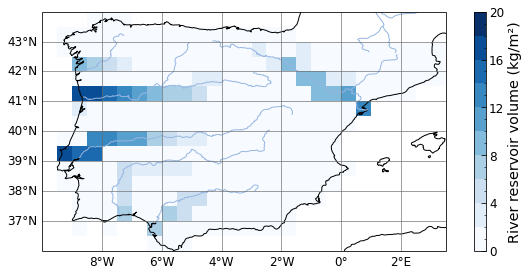
\includegraphics[width=\textwidth]{images/chap3/maps/streamr_subgrid.png}
        \end{subfigure} &
        \begin{subfigure}[b]{0.33\textwidth}
            \caption{River reservoir\\(annual mean, \native)}
            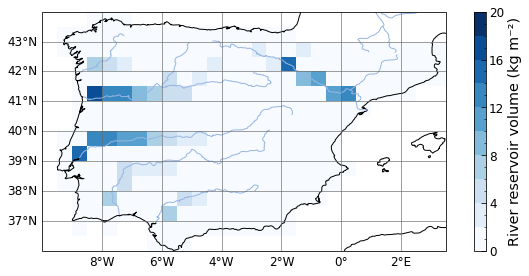
\includegraphics[width=\textwidth]{images/chap3/maps/streamr_interp.png}
        \end{subfigure} &
        \begin{subfigure}[b]{0.33\textwidth}
            \caption{River reservoir difference \\(\native -\std)}
            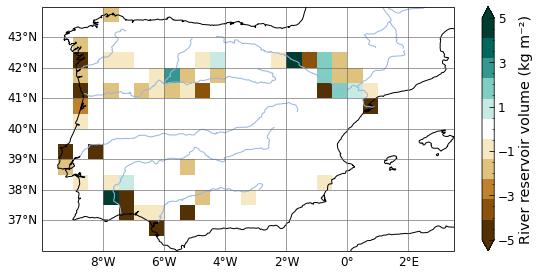
\includegraphics[width=\textwidth]{images/chap3/maps/streamr_diff.png}
        \end{subfigure} \\
        
        \begin{subfigure}[b]{0.33\textwidth}
            \caption{River discharge\\(annual mean, \std)}
            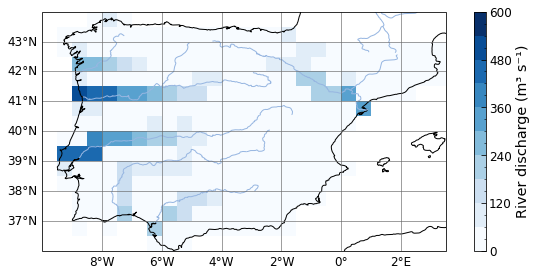
\includegraphics[width=\textwidth]{images/chap3/maps/hydrographs_subgrid.png}
        \end{subfigure} &
        \begin{subfigure}[b]{0.33\textwidth}
            \caption{River discharge\\(annual mean, \native)}
            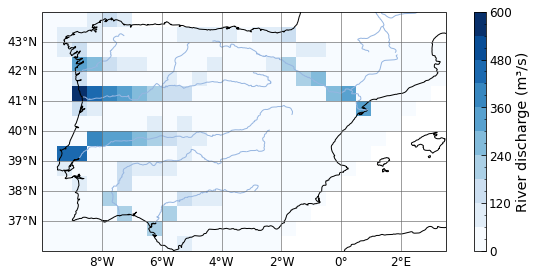
\includegraphics[width=\textwidth]{images/chap3/maps/hydrographs_interp.png}
        \end{subfigure} &
        \begin{subfigure}[b]{0.33\textwidth}
            \caption{River discharge difference \\(\native -\std)}
            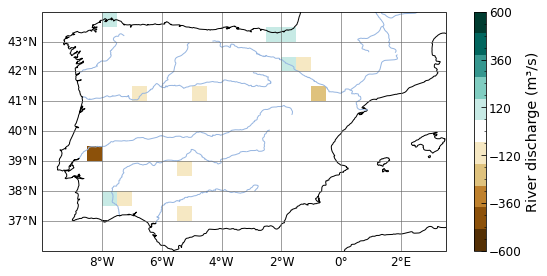
\includegraphics[width=\textwidth]{images/chap3/maps/hydrographs_diff.png}
        \end{subfigure} \\
    \end{tabular}
    \caption{Annual mean (2003-2012) of reservoir volumes and river discharge for \std (\noirr), \native (\noirr) and difference between them. 
    The scale for (l) was deliberately chosen much smaller than (j) and (k) to highlight differences between the two simulations.}
    \label{fig:routing_reservoirs_halfdeg}
\end{figure}

The comparison of the mean volumes for the groundwater and overland reservoirs (Fig. \ref{fig:routing_reservoirs_halfdeg}a-f) shows differences only on coastal grid cells, which are very low in \std but can have significant values in \native, particularly in the northern strip of the Peninsula. Considering these are mostly moutainous regions which receivre large precipitation, and therefore exhibit high drainage and surface runoff, the values computed by \native in this region are in the expected order of magnitude, whereas the values in \std are 10 to 70 times smaller.
Therefore, the cause considered most likely is that \std does not hold water in the reservoir of these coastal grid cells as long as it should, compared to neighbouring non-coastal grid cells. In the routing scheme, coastal grid cells have to be managed differently since they flow to the sea rather than to the river reservoir of the downstream grid cell. It is therefore possible that different modelling or implementation choices were made when developping the code for \std. Another possible explanation is that, as explained in Section\ref{sec:routing_methods} \std preprocesses the DEM, which could possibly alter the slope on these coastal grid cells in a way that empties them much faster than expected.
However these discrepancies are still not completely understood and still under investigation, in collaboration with Antoine Bierjon (research engineer at IPSL), to clarify their cause and determine whether they introduced errors or corrected existing flaws of the previous code for coastal grid cells.

%old possible explanation with Contfrac, further tested and doesn't seem to be the problem...
% These differences are thought to be the consequence of a different handling of water quantities and their units in \native compared to \std. 
% As detailed in Section \ref{sec:irrig_interp_variables}, in \native, drainage and surface runoff are computed on the ORCHIDEE grid, in $kg \cdot m^{-2}$ (equivalent to $mm$ over the grid cell) and converted to absolute water quantities (in $kg$) before being interpolated to the DEM grid. These absolute quantities are routed on the DEM grid and the new water quantities in the reservoirs are reinterpolated to the ORCHIDEE grid (even when the two grids have the same resolution). To express them as an areal value, in $kg \cdot m^{-2}$, the absolute water quantity has to be divided by the area of the grid cell. It is considered likely that this back-and-forth interpolation and change of units introduces the differences, by accounting for continental fraction (to obtain the exact area on coastal points) whereas in \std this was not necessary since all computations were on the same grid cell. Such subtleties in the code were introduced to enable compatibility with any DEM grid.

Since this issue affected only the groundwater and overland reservoirs and was located only on coastal grid cells, it was considered that for the purpose of this work, the impacts should not affect the results substantially and that \native could be used in its current version.
%todo:continuer à clarifier avec Antoine et/ou Yann pour mieux expliquer...? 

\hfill

Regarding the river reservoir (Fig. \ref{fig:routing_reservoirs_halfdeg}g-i), a new modelling choice was made on coastal grid cells. In \std, there was a river reservoir for these grid cells, whereas it was removed in \native as schematized in Fig. \ref{fig:coastal_routing_behaviour}. This choice was made during the development of the code and might be changed in future versions to ensure consistency with the other two reservoirs. It is responsible for the large differences in river reservoir on large river outlets (Fig. \ref{fig:routing_reservoirs_halfdeg}i).

However, this difference does not translate to values of river discharge since it is still computed in coastal grid cells in \native using the outflow from the river reservoir of the upstream grid cells, and from the groundwater and overland reservoirs (Fig. \ref{fig:routing_reservoirs_halfdeg}j-l). River discharge is also larger in \native than in \std on all coastal grid cells, although it must be noted that the scale for the river discharge was specifically chosen to be able to visualise this difference (Fig. \ref{fig:routing_reservoirs_halfdeg}l). This is very likely the consequence of the differences noticed in the groundwater and overland reservoir, which both contribute to the discharge and are much larger in \native for coastal grid cells, as explained previously.

% The way to compute river discharge in these coastal points is also slightly different in \native, as it includes the flow from the river reservoir of the upstream grid cell, as well as the flow from the groundwater and overland reservoirs of the grid cell, whereas drainage and surface runoff were considered to flow directly in the ocean in \std. This explains why discharge values are or similar order of magnitude but larger in \native (Fig. \ref{fig:routing_reservoirs_halfdeg}l). Figure \ref{fig:coastal_routing_behaviour} schematizes the differences in implementation that explain the differences seen in the river reservoir and in the discharge on coastal grid cells.

\begin{figure}[htbp]
    \centering
    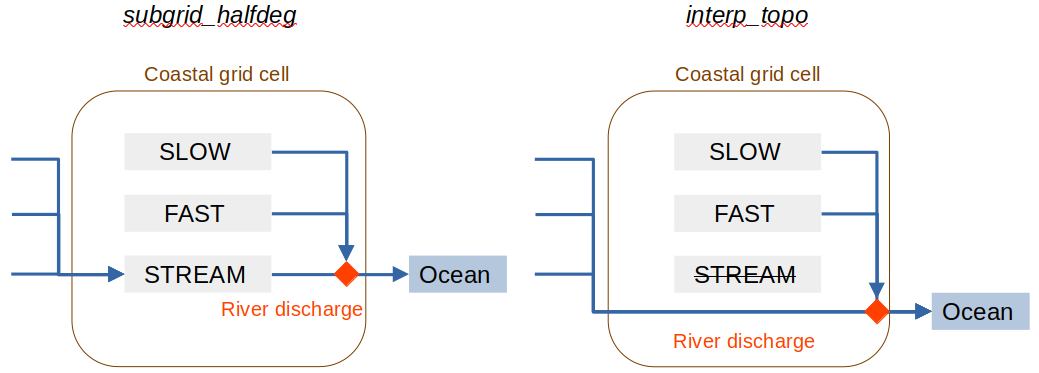
\includegraphics[width=\textwidth]{images/chap3/coastal_routing_behaviour_v3.png
}
    \caption{Differences in implementation between \std and \native on coastal grid cells.}
    \label{fig:coastal_routing_behaviour}
\end{figure}

\subsection{Differences in routing path, average impacts on reservoir volumes}
Appart from coastal grid cells, the most noticeable discrepancy on the river reservoir and river discharge is that some non-coastal points have different values in both routing versions. It can be seen on Fig. \ref{fig:routing_reservoirs_halfdeg}j-l particularly that the water does not flow exactly in the same path, meaning that the DEM is not interpreted exactly in the same way. 
This has been attributed to preprocessings of the DEM implemented in \std, mentionned in Section \ref{sec:routing_methods}, which were specific to its structure and therefore not implemented in \native. In the large rivers where there are differences, \native seems to use shorter paths that \std, often flowing diagonally to the next grid cell whereas \native takes two 90° turns instead due to its altered routing path. In most of the domain, on annual average, this leads to smaller amounts of water in the river reservoir and smaller discharge in \native compared to \std, as clearly visible on the Duero river in Fig. \ref{fig:routing_reservoirs_halfdeg}l.

%figure : 3 time series (3 reservoirs)on average over the IP for both routings
\begin{figure}[htbp]
    \centering
    \begin{subfigure}[b]{0.32\textwidth}
        \caption{Groundwater reservoir average}
        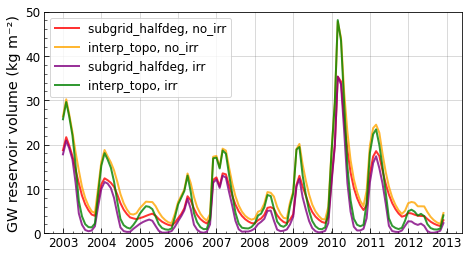
\includegraphics[width=\textwidth]{images/chap3/time_series/slowr_time_series.png}
    \end{subfigure}
    \begin{subfigure}[b]{0.32\textwidth}
        \caption{Overland reservoir average}
        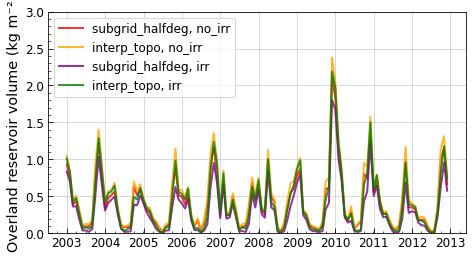
\includegraphics[width=\textwidth]{images/chap3/time_series/fastr_time_series.png}
    \end{subfigure}
    \begin{subfigure}[b]{0.32\textwidth}
        \caption{River reservoir average}
        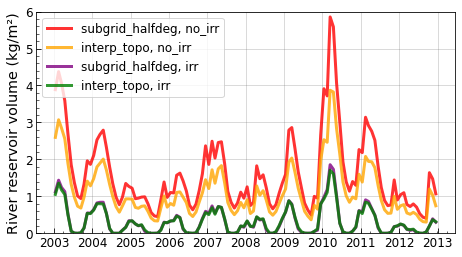
\includegraphics[width=\textwidth]{images/chap3/time_series/streamr_time_series.png}
    \end{subfigure} \\

    \begin{subfigure}[b]{0.32\textwidth}
        \caption{Groundwater reservoir average seasonal cycle}
        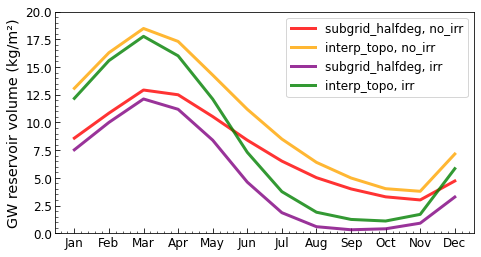
\includegraphics[width=\textwidth]{images/chap3/time_series/slowr_seasonal_cycle.png}
    \end{subfigure}
    \begin{subfigure}[b]{0.32\textwidth}
        \caption{Overland reservoir average seasonal cycle}
        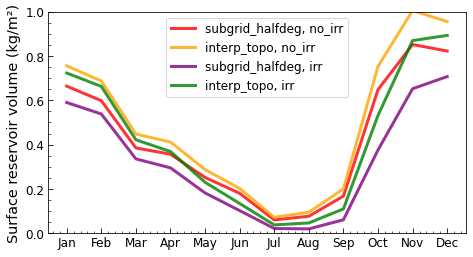
\includegraphics[width=\textwidth]{images/chap3/time_series/fastr_seasonal_cycle.png}
    \end{subfigure}
    \begin{subfigure}[b]{0.32\textwidth}
        \caption{River reservoir average seasonal cycle}
        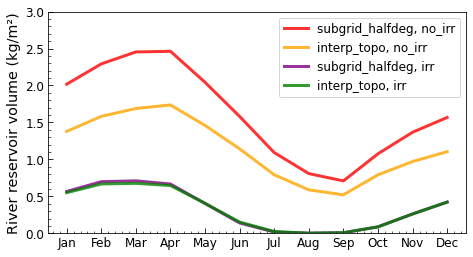
\includegraphics[width=\textwidth]{images/chap3/time_series/streamr_seasonal_cycle.png}
    \end{subfigure}
    \caption{Time series and seasonal cycles of reservoir volumes on average over the Iberian Peninsula domain.}
    \label{fig:reservoir_time_series}
\end{figure}

On average over the Peninsula, the differences noticed above are visible in the groundwater and overland reservoirs where \native has larger volumes due to water in coastal grid cells (Fig. \ref{fig:reservoir_time_series}a, b). On the river reservoir however, \std has larger volumes, mostly due to the absence of this reservoir on coastal points with river outlets, which are among the grid cells with the largest volumes in \std.
If all coastal grid cells were to be removed from the average (not shown)%option: faire la figure ? ou annexe ?
, there would be no difference on the groundwater and overland reservoirs, and a much smaller difference on the river reservoir, although \std still has more water stored in this reservoir than \native, particularly in winter and spring, when there is more rain in the region. This confirms the previous observation that water follows shorter paths to the sea in \native and therefore, does not remain in the river reservoir as long as in \std.
\subsection{Simulated irrigation and river discharge}

In the \irr simulations (purple and green lines in Fig. \ref{fig:reservoir_time_series}), all reservoirs are partly depleted by the irrigation withdrawals. For the groundwater and overland reservoirs, the differences between \std and \native mostly remain, since they are located in coastal grid cells, which are seldom intensely irrigated.
Regarding the river reservoir (Fig. \ref{fig:reservoir_time_series}f), \std simulates much lower volumes in the \irr than in \noirr simulation (-75\% in winter and complete depletion in summer). This decrease is also seen with \native, and the differences between the two routing versions almost disappear. This is consistent with the source of these differences, since the \irr simulations exhibit much lower volumes in rivers in general, the discrepancies due to the routing graph and coastal grid cells have much less impact on the average volume over the domain.

%figure : 3 maps of simulated irrigation (subgrid, interp, diff), TS and SC of irrig for both simulations
\begin{figure}[htbp]
    \centering
    \begin{subfigure}[b]{0.32\textwidth}
        \caption{Irrigation annual mean\\(\std)}
        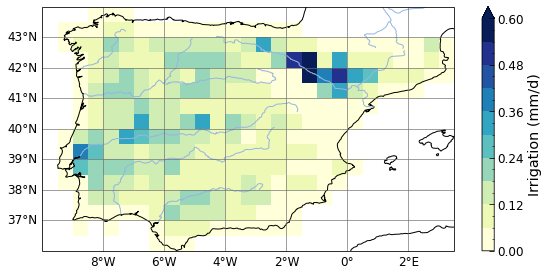
\includegraphics[width=\textwidth]{images/chap3/maps/irrigation_subgrid.png}
    \end{subfigure}
    \begin{subfigure}[b]{0.32\textwidth}
        \caption{Irrigation annual mean\\(\native)}
        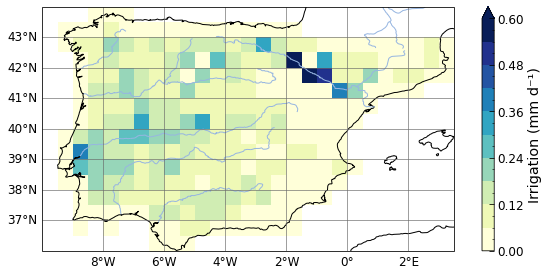
\includegraphics[width=\textwidth]{images/chap3/maps/irrigation_interp.png}
    \end{subfigure}
    \begin{subfigure}[b]{0.32\textwidth}
        \caption{Irrigation difference\\(\native -\std)}
        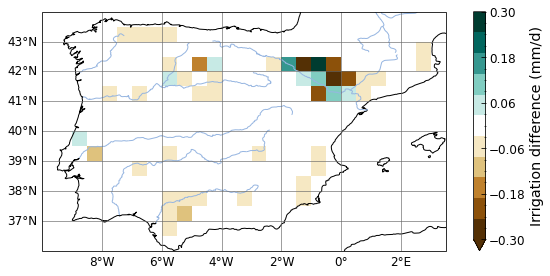
\includegraphics[width=\textwidth]{images/chap3/maps/irrigation_diff.png}
    \end{subfigure} \\

    \begin{subfigure}[b]{0.48\textwidth}
        \caption{Irrigation (Iberian Peninsula average)}
        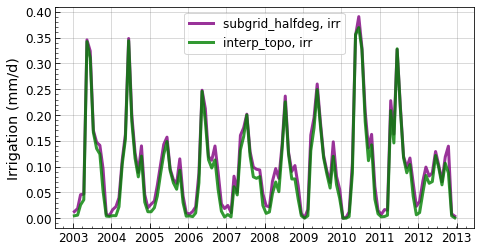
\includegraphics[width=\textwidth]{images/chap3/time_series/irrigation_time_series.png}
    \end{subfigure}    
    \begin{subfigure}[b]{0.48\textwidth}
        \caption{Irrigation average seasonal cycle}
        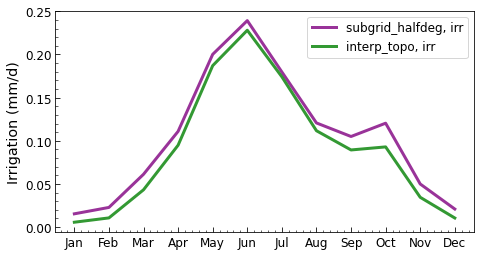
\includegraphics[width=\textwidth]{images/chap3/time_series/irrigation_seasonal_cycle.png}
    \end{subfigure}

    \caption{Simulated irrigation in \std and \native. Annual mean for both simulations (a,b) and difference (c). Average time series (d) and seasonal cycle (e) over the Iberian Peninsula.}
    \label{fig:irrigation_halfdeg_eval}
\end{figure}

Both simulations show a similar simulated irrigation (Fig. \ref{fig:irrigation_halfdeg_eval}), but the differences on reservoir volumes affect the available water, and therefore irrigation. This is particlarly visible in the Ebro valley where some grid cells are highly irrigated in one simulation and not in the other. This is due to the aforementionned differences in the routing graph, which affect the path of the Ebro river (Fig. \ref{fig:irrigation_halfdeg_eval}c), the main source for irrigation withdrawals in the region (Fig. \ref{fig:irrig_inputs}b).
On average over the domain (Fig. \ref{fig:irrigation_halfdeg_eval}d, e) \std exhibits slightly higher volumes of irrigation than \native, which is consistent with the higher volumes in the river reservoir. As previously mentionned, the differences seen in the reservoirs on coastal grid cells seem to have little impacts on the irrigated volumes, since these regions are seldom intensely irrigated (Fig. \ref{fig:irrig_inputs}a). 

In both simulations, irrigation progressively increases in spring, decreases in July and August, before increasing once again in autumn (Fig. \ref{fig:irrigation_halfdeg_eval}e). Although this section does not aim to provide an in-depth evaluation of the simulated irrigation, it must be noted that this seasonal cycle is not realistic and does not reflect the irrigation demand, which is highest in July and August. This drop in irrigation in summer can be explained by a lack of available water in the reservoirs, which that they are depleted by the end of June (Fig. \ref{fig:reservoir_time_series}d-f). Even though demand remains high, irrigation can not be sustained all summer, and it is only in autumn, when reservoirs are partly replenished by precipitation, that the irrigation demand can once again be satisfied. This aspect was a first hint that the irrigation parameterization might have to be adjusted to better reflect irrigation over the study area, which is further discussed in Section \ref{sec:forcing_irr_reduced}.

%figure : river discharge seasonal cycle for 4 stations (large rivers but not Guadalquivir...), 2 routing versions, irr and no_irr for each
\begin{figure}[htbp]
    \centering
    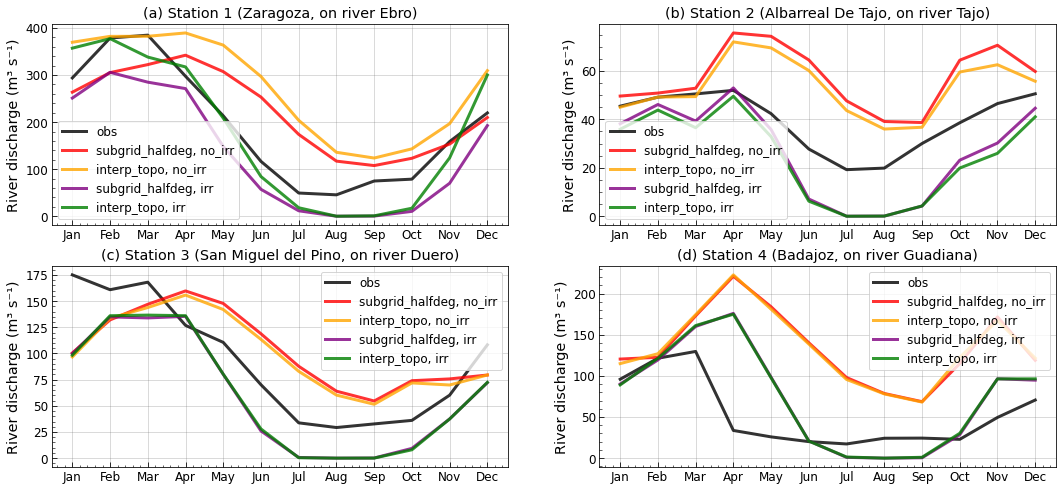
\includegraphics[width=\textwidth]{images/chap3/river_discharge/halfdeg_4stations_SC.png}
    \caption{Mean seasonal cycle (2003-2012) of river discharge in GRDC observations and four simulations, with \native and \std, each with and without irrigation.}
    \label{fig:halfdeg_stations_SC}
\end{figure}

The seasonal cycle of river discharge reflects the general agreement of the two routing versions. Without irrigation, the red and yellow lines follow each other closely, and with irrigation, the purple and green are also very similar. Some differences persist, due to the differences in the routing graph already described, mostly for the Ebro river since the station is downstream of several important discrepancies visible on Fig. \ref{fig:routing_reservoirs_halfdeg}l.
%todo:add the general overestimation without irrig, limits in representation of dam storage ; slight delay in winter peak...

\subsection{Conclusions on \native routing consistency}
This comparison of the \native routing version with \std showed that this new version is generally reproducing the modelling principles correctly, but several differences were identified between the two versions. All three reservoirs are handled differently in \native on coastal grid cells, which affects the average volumes stored over the Iberian Peninsula, but does not have a significant impact on irrigation or river dicharge. However, differences in the path followed by water as it flows from one grid cell to another in the river reservoirs are also clearly identified in large rivers of the Peninsula. This leads to local changes in the simulated river dicharge, and slightly less water stored in the river reservoir by \native since it simulated shorter paths in several occurrences. These discrepancies also have an impact on irrigation since it is strongly reliant on the volumes of water available in the river reservoir, but this impact remains limited on average over the domain.

\section{Calibration over the Iberian Peninsula}
\label{section:calib}

Once the general consistency of the \native routing had been assessed, it became possible to evaluate the specific setup that would be used for the coupled simulation, using the MERIT DEM at 2km resolution and accounting for irrigation. To use irrigation, the routing time step must be the same as the time step of ORCHIDEE, which is 15mn (900s) in coupled simulations. 

This calibration was initially focused on the three time constants of the routing reservoirs: TCST\_SLOW, TCST\_FAST, TCST\_STREAM. Although these parameters should theoretically be independent of the spatial and temporal time steps, and of the DEM used as input, 
In particular, the ORCHIDEE routing scheme had never been used with a high-resolution topography like the MERIT DEM at 2-km resolution, since the \std routing ran only with the 0.5° resolution DEM used in the previous section, and often with a 24-hours routing time step. Multiple tests were therefore carried to identify an appopriate set of time constants for the reservoirs.
Moreover, the sensitivity of river discharge to the activation of irrigation was identified as very important, with large differences in the responses depending on the intensity of irrigation demand. As a consequence, the parameter \betairrig, which defines the soil moisture target in the irrigation scheme, was also included in this calibration and modified compared to the default version of the model.

\subsection{Simulation experiments}

At the begining of the calibration, three reference sets of TCST parameters (presented in Table \ref{table:tcst_refs}) were considered:
\begin{itemize}
\item The values established during an initial calibration of the \native routing performed over the Danube basin, which focused only on river discharge observations \citep{kilic_evaluation_2023}.
\item The default values used by the \std routing on a global scale, which were used in the previous section with the 0.5° DEM. These values were identified empirically by a calibration study over the Senegal river basin and validated globally in \citet{ngo-duc_53-year_2005, ngo-duc_validation_2007} using river discharge and groundwater measurements from Gravity Recovery and Climate Experiment (GRACE) satellite data.
\item The values used for regional studies with the \textit{subgrid\_HTU} routing \citep{rinchiuso_improving_2022, huang_multi-objective_2024}.
\end{itemize}

\begin{table}[h]
\centering
\begin{tabular}{|l|c|c|c|}
\hline
\textbf{} & \textbf{TCST\_SLOW} & \textbf{TCST\_FAST} & \textbf{TCST\_STREAM} \\ \hline
Initial \native calibration & 1.2 & 0.9 & 0.03 \\ \hline
\std default values & 25 & 3 & 0.24 \\ \hline
\textit{Subgrid\_HTU} calibration & 600 & 80 & 6.3 \\ \hline
\end{tabular}
\caption{Reference parameter sets considered to calibrate the \native routing ($day \cdot km^{-1}$).}
\label{table:tcst_refs}
\end{table}

In these three sets of values, there is approximately an order of magnitude between the three time constants, and very significant differences (one or two orders of magnitude) between each set. 
This can be explained by the different DEMs used, the way HTUs are defined, and the calibration choices that led to these sets of values.%option:compléter explication ? 

Three initial experiments were defined, based on these ratios:\\$TCST\_SLOW \approx 10 \times TCST\_FAST \approx 100 \times TCST\_STREAM$.
Table \ref{table:tcst_exp} presents these three sets of values based on the orders of magnitude of each of the reference value sets (TCST1, TCST2, TCST3), as well as the one selected after the calibration (TCST4), whose development steps are detailed hereafter.

\begin{table}[h]
\centering
\begin{tabular}{|l|c|c|c|}
\hline
\textbf{} & \textbf{TCST\_SLOW} & \textbf{TCST\_FAST} & \textbf{TCST\_STREAM} \\ \hline
TCST1 & 3 & 0.3 & 0.03 \\ \hline
TCST2 & 30 & 3 & 0.3 \\ \hline
TCST3 & 300 & 30 & 3 \\ \hline
TCST4 & 700 & 100 & 0.1 \\ \hline
\end{tabular}
\caption{Value sets of the simulations for the calibration of the \native routing ($day \cdot km^{-1}$).}
\label{table:tcst_exp}
\end{table}

Four simulations without irrigation were therefore carried out with these four sets of TCST values over the period 2000-2012 and analysed over 2003-2012.

\subsection{Reservoir volumes and time constants}

Volumes in each of the reservoirs were first compared to the volumes simulated by the \std routing. As a reminder, this version, with the 0.5° DEM, has long been used in ORCHIDEE and was evaluated against groundwater reference products from GRACE, as well as river discharge observations  \citep{ngo-duc_53-year_2005, ngo-duc_validation_2007}.
It is also the version that was used for the evaluation and validation of the irrigation scheme at global scale \citep{arboleda-obando_validation_2024}, which makes it a relevant reference for the reservoir volumes since available water is a major driver of simulated irrigation in the model. 

On average over the Peninsula, for the groundwater and Overland reservoirs, the TCST3 simulation showed values closest to \std (Fig. \ref{fig:reservoir_time_series_tcsts}a, b, d, e), while TCST1 and TCST2 hold almost no water in these reservoirs, meaning that they flow more quickly in the river reservoir. On the river reservoir however (Fig. \ref{fig:reservoir_time_series_tcsts}c, f), TCST3 is one order of magnitude above the other simulation, including \std, hinting that the value to TCST\_STREAM is too large for this reservoir, meaning that water circulates too slowly. This is confirmed looking at river discharge (Fig. \ref{fig:merit_tcsts_stations_SC}), as TCST3 cannot reproduce the observed structure of the seasonal cycle for any of the four rivers considered. These results, as well as a few intermediate tests not shown here, led to the choice of a new set of parameters (TCST4), which has values similar to TCST3 for the groundwater and overland reservoirs, but closer to TCST2 (even slightly faster) for the river reservoir (\ref{table:tcst_exp}), shown in red in Fig. \ref{fig:reservoir_time_series_tcsts} and \ref{fig:merit_tcsts_stations_SC}.
Average simulated volumes for TCST4 are clos to \std on all reservoirs, and match discharge observations with similar performance to TCST1 and TCST2.
%option:add metrics ? KGE, BIAS

It can be noted that the performance of TCST1 for river dischage is good, but that it holds almost no water in the groundwater and overland reservoirs, suggesting that this previous calibration with the 2-km MERIT DEM focusing only on matching discharge observations \citep{kilic_evaluation_2023} neglected some aspects of the routing scheme and effectively calibrated only TCST\_STREAM.


%figure : 3 time series (3 reservoirs) on average over the IP for 4 tcsts and std as reference
\begin{figure}[htbp]
    \centering
    \begin{subfigure}[b]{0.32\textwidth}
        \caption{Groundwater reservoir average}
        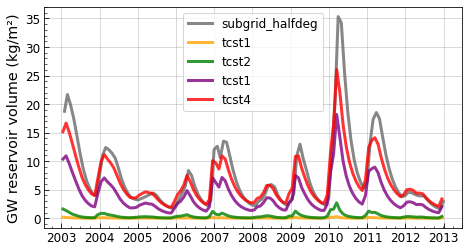
\includegraphics[width=\textwidth]{images/chap3/time_series/slowr_time_series_tcsts.png}
    \end{subfigure}
    \begin{subfigure}[b]{0.32\textwidth}
        \caption{Surface water average}
        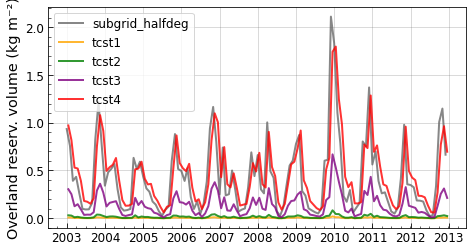
\includegraphics[width=\textwidth]{images/chap3/time_series/fastr_time_series_tcsts.png}
    \end{subfigure}
    \begin{subfigure}[b]{0.32\textwidth}
        \caption{River reservoir average}
        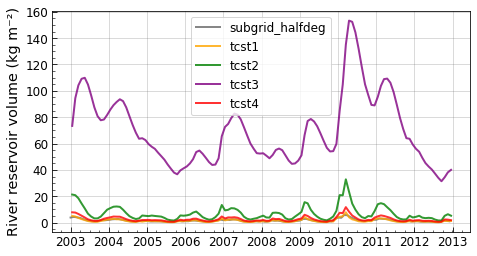
\includegraphics[width=\textwidth]{images/chap3/time_series/streamr_time_series_tcsts.png}
    \end{subfigure} \\

    \begin{subfigure}[b]{0.32\textwidth}
        \caption{Groundwater reservoir average seasonal cycle}
        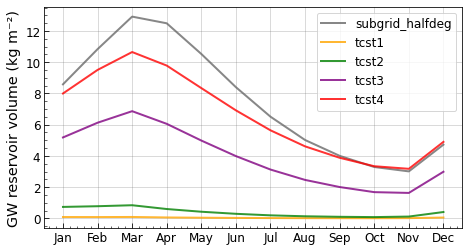
\includegraphics[width=\textwidth]{images/chap3/time_series/slowr_seasonal_cycle_tcsts.png}
    \end{subfigure}
    \begin{subfigure}[b]{0.32\textwidth}
        \caption{Overland reservoir average seasonal cycle}
        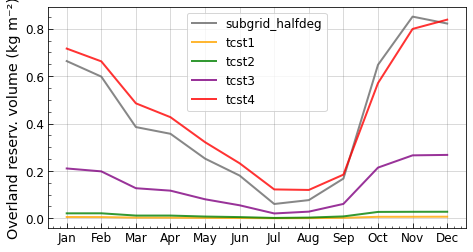
\includegraphics[width=\textwidth]{images/chap3/time_series/fastr_seasonal_cycle_tcsts.png}
    \end{subfigure}
    \begin{subfigure}[b]{0.32\textwidth}
        \caption{River reservoir average seasonal cycle}
        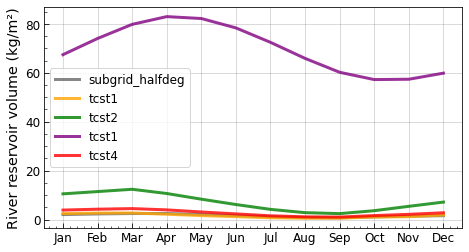
\includegraphics[width=\textwidth]{images/chap3/time_series/streamr_seasonal_cycle_tcsts.png}
    \end{subfigure}
    \caption{Time series and seasonal cycles of reservoir volumes on average over the Iberian Peninsula domain.}
    \label{fig:reservoir_time_series_tcsts}
\end{figure}

%figure : river discharge seasonal cycle for 4 stations (large rivers but not Guadalquivir...), 2 routing versions, irr and no_irr for each
\begin{figure}[htbp]
    \centering
    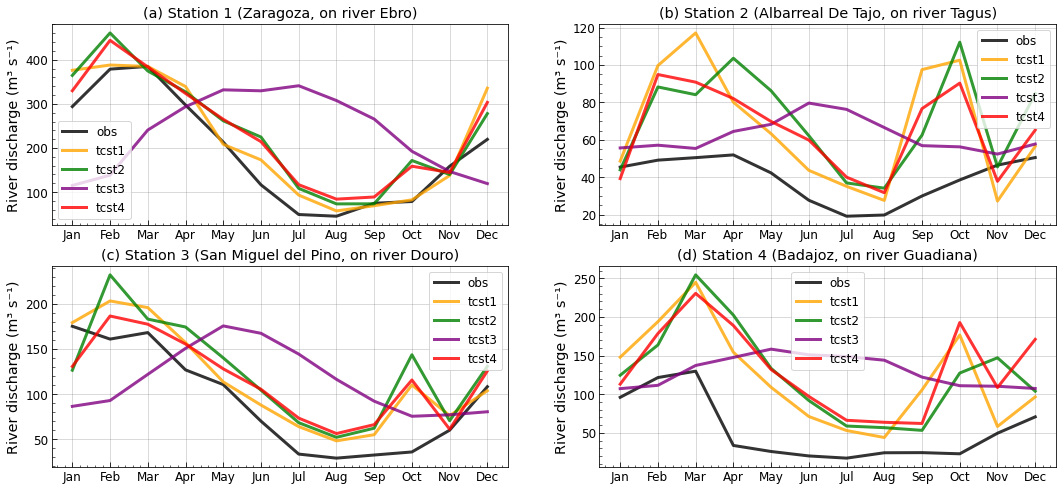
\includegraphics[width=\textwidth]{images/chap3/river_discharge/merit_tcst_4stations_SC.png}
    \caption{River discharge mean seasonal cycle (2003-2012) with four sets of TCST parameters.}
    \label{fig:merit_tcsts_stations_SC}
\end{figure}

Further tests for the choice of parameters were considered, to explore if the performance of the \native routing with MERIT DEM could be further improved regarding river discharge, but sensitivity experiments were first conducted, using the TCST4 parameter set, to assess the relevance of a finer tuning of the TCST parameters.

\subsection{Impacts of atmospheric forcing and irrigation on river discharge}
\label{sec:forcing_irr_reduced}

\begin{figure}[htbp]
    \centering
    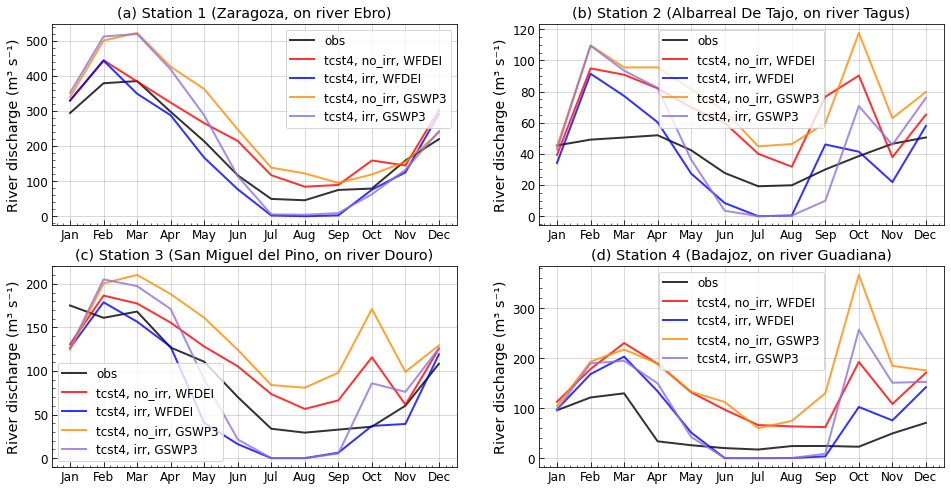
\includegraphics[width=\textwidth]{images/chap3/river_discharge/merit_forcing_4stations_SC.png}
    \caption{River discharge mean seasonal cycle (2003-2012) with GSWP3 and WFDEI forcings, with ant without irrigation.}
    \label{fig:merit_forcing_stations_SC}
\end{figure}

The impacts of the atmospheric forcing used and of irrigation were assessed jointly with four simulations, all with the TCST4 parameter set, using two atmospheric forcings (WFDEI and GSWP3), each with and without irrigation. Considering the availability of GSWP3, simulations were only run until 2010.

The results (Fig. \ref{fig:merit_forcing_stations_SC}) show a response to both changes but a stronger impact of irrigation, which strongly reduces discharge, except in winter. The WFDEI and GSWP3 forcing produce seasonal cycles with similar structures but using the GSWP3 forcing leads to larger discharge in the winter peak for the Ebro and Douro basin, as well in the peak of autumn precipitation in the Tagus, Douro and Guadiana basins. These regional and sesonal specificities reflect the differences in precipitation between the two forcings. 
%option:show yearly or seasonal maps of precip ? side by side, diff ?
In summer, the \noirr and \irr simulations with the two forcings are similar, especially with irrigation, which depletes the river reservoir, reducing discharge to near-zero for the four rivers.

The strengths of these responses, compared to the differences in the parameter sets explored in Fig. \ref{fig:merit_tcsts_stations_SC} justified the decision not to pursue finer tuning of the TCST parameters, which would be too dependent on the forcing or the activation of irrigation. The TCST4 parameter set was considered an acceptable option for the routing scheme, and it was decided to include the parameterization of irrigation in the calibration. 

\begin{figure}[htbp]
    \centering
    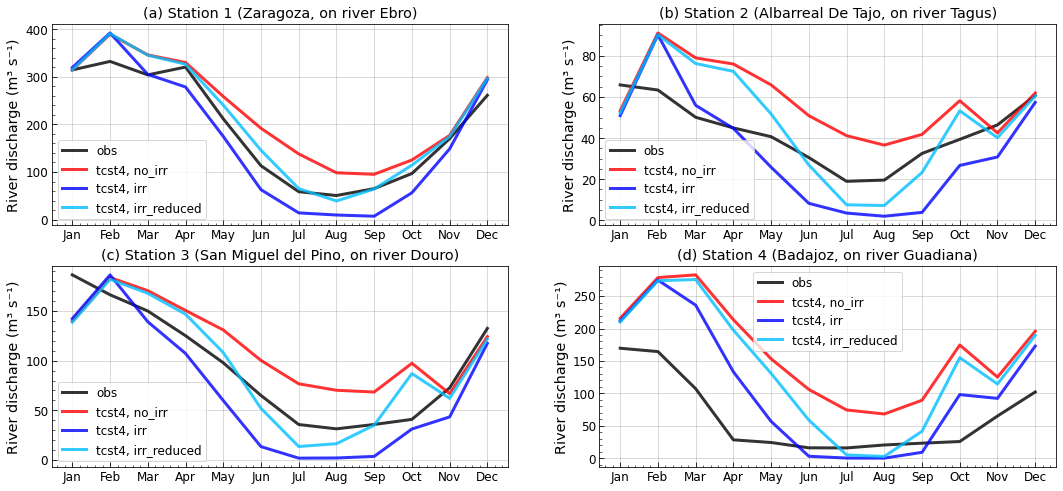
\includegraphics[width=\textwidth]{images/chap3/river_discharge/merit_irr_4stations_SC.png}
    \caption{River discharge mean seasonal cycle (2003-2010) in the \noirr, \irr and \textit{irr\_reduced} simulations.}
    \label{fig:merit_irr_stations_SC}
\end{figure}

The global evaluation of the ORCHIDEE irrigation scheme \citep{arboleda-obando_validation_2024} identified the \betairrig parameter as the main driver of simulated irrigation. This parameter conditions the soil moisture target as a fraction of soil moisture at field capacity. The default value selected for global simulations was \betairrig = 0.9. However, this value was chosen as an average on the global scale, meant to reflect a large diversity of irrigation practices, including flooding methods in rice paddies, which is common in intensely irrigated regions of northern India and China. For such practices, \betairrig = 1.2 would be more appropriate to represent the irrigation withdrawals properly. In the Iberian Peninsula however, the limited water supply and semiarid climate favor less water intensive methods (drip or sprinkler irrigation) which would be better represented with lower values of \betairrig. The value of $0.9$ was selected as a way to center the global biases compared to reference products on zero, acknowledging that this value was too low for some regions and too high for others.

This is why other values were explored for the calibration over the Iberian Peninsula, as well as to limit the unrealistic depletion of rivers in summer. Fig. \ref{fig:merit_irr_stations_SC} shows three simulations, all with the WFDEI forcing and TCST4 set of parameter for routing, but with different options for irrigation: \noirr, \irr (default value \betairrig = 0.9) and \textit{irr\_reduced} with \betairrig = 0.6. 
This simulation limits the depletion in summer and yields much better performance in the Ebro basin, which is the most very intensely irrigated region, and largely depends on water from river (as opposed to groundwater) for irrigation.
This reduced irrigation also seems more consistent when looking at the seasonal cycle of irrigation (Fig. \ref{fig:merit_irr_reduced}c). In the default \irr simulation, high volumes are withdrawn in the spring but irrigation drops in summer, which is the season where irrigation demand is the highest. This is due to a lack of available water in the reservoirs in the irrigated regions in summer, which are depleted too quickly when using \betairrig = 0.9. The effect of the river reservoir depletion is also visible on the summer river discharge of Fig. \ref{fig:merit_irr_stations_SC} which falls to near-zero for the four rivers considered.

To summarize, the \textit{irr\_reduced} setup simulates a lower demand in irriation and therefore less irrigation overall, but it avoids an early depletion of the reservoirs, yielding a more consistent seasonal cycle of irrigation and matching discharge observation better in spring and summer.
%option : also show root_deficit to demonstrate that large Beta leads to much larger demand

%figure : maps of irrig in irr and irr_reduced, and seasonal cycle of irrig over IP for both sims
\begin{figure}[htbp]
    \centering
    \begin{subfigure}[b]{0.32\textwidth}
        \caption{Mean irrigation in \irr.\\ } 
        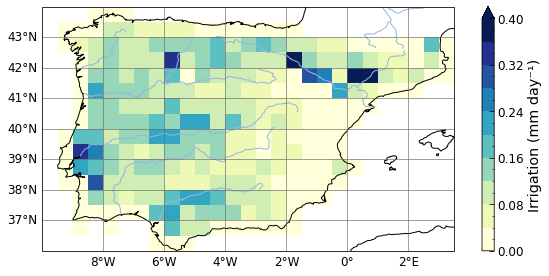
\includegraphics[width=\textwidth]{images/chap3/maps/irrigation_ave_tcst4_irr.png}
    \end{subfigure}
    \begin{subfigure}[b]{0.32\textwidth}
        \caption{Mean irrigation in \textit{irr\_reduced}.} 
        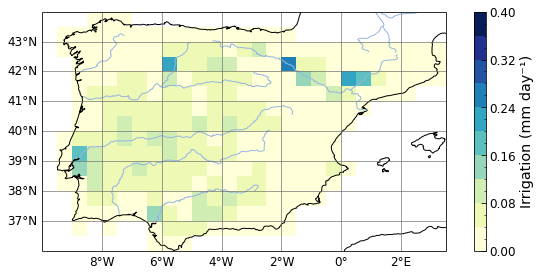
\includegraphics[width=\textwidth]{images/chap3/maps/irrigation_ave_tcst4_irr_reduced.png}
    \end{subfigure}
    \begin{subfigure}[b]{0.32\textwidth}        
        \caption{seasonal cycle of irrigation.} 
        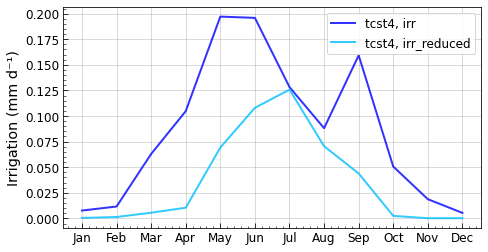
\includegraphics[width=\textwidth]{images/chap3/time_series/irrigation_seasonal_cycle_irr_reduced.png}
    \end{subfigure}
    \caption{Simulated irrigation in the \irr and \textit{irr\_reduced} simulations (2003-2012).}
    \label{fig:merit_irr_reduced}
\end{figure}

\pagebreak

\section{Chapter conclusions}

This chapter presents the evaluation and calibration of the new version of the routing scheme (\native) using ORCHIDEE offline simulations over the Iberian Peninsula. This was a necessary step to prepare for coupled simulations, which provided a finer understanding of the behaviour of the routing scheme with different DEMs, and also highlighted the interdependency between the irrigation parameterization, the routing reservoirs, and river discharge. 

This calibration and evaluation work first showed that the new routing code mostly behaves similarly to the pre-existing version (\std) if given the same time step, input map, and parameters, although some differences were identified on the coastal grid cells. Differences in the routing path also appeared between \std and \native, leading to local differences in discharge and irrigation.

The \native routing was then used with a high-resolution (2 km) DEM over the Iberian Peninsula, and several options were tested for the reservoir time constants. 
Comparison of reservoir volumes with the previous version of the routing (\std), which served as a first reference, highlighted the limits of a previous calibration by \citet{kilic_evaluation_2023} regarding these two reservoirs, and allowed the identification of values for TCST\_SLOW and TCST\_FAST to simulate similar water volumes on average over the Peninsula. This was essential because of the dependance of the irrigation scheme on the available water in the routing reservoirs.
Using discharge observations, the value of TCST\_STREAM was then adjusted to correctly represent the seasonal cycle of the major rivers of the Iberian Peninsula.

Sensitivity experiments highlighted the very large response of river discharge to the activation of irrigation (except in winter), and a significant yet more moderate response to the atmospheric forcing used for the calibration. 
The magnitude of these sensitivities also contributed to the decision not to further calibrate the TCST values, as their impact on simulated river discharge performance remains limited compared to that of irrigation.
As a consequence, the \betairrig parameter of the irrigation scheme was also included in the calibrated parameters, and 0.6 was identified as a more suitable value than the default value of 0.9. This option avoids depletion of the reservoirs, which makes the seasonal cycle of irrigation more consistent and enables better agreement with observation for discharge in summer. As hypothesized in \citet{arboleda-obando_validation_2024} this value is considered more consistent with a representation of irrigation practices in the region.

Therefore, the set of parameters from the simulations \textit{tcst4\_no\_irr} and \textit{tcst4\_irr\_reduced} were used to study the impact of irrigation in the coupled simulations presented in Chapter \ref{chap:monthly}.
%over


\chapter{Influence of lateral boundary conditions on the consistency of the ICOLMDZOR LAM}
\label{chap:forcing}
\minitoc
\pagebreak
% This section presents the inconsistencies identified in the LAM transition zone, several possible options explored to mitigate them, and their impact on the LAM free zone and the Iberian Peninsula subdomain. In all the section, the ERA5 reanalysis is used as a reference. Although it is not considered the most realistic reference for all variables, the study of the inconsistencies mostly focused on the spatial structure of the variables, rather than on the absolute values.
For this purpose, ERA5 has two advantages: it is available over all the simulation domain, at a resolution similar to the simulations (0.25° is close to 25km in midlatitudes), and provides all the variables of the model.
While most figures presented are maps of biases relative to ERA5 for six variables of interest, their values in the reanalysis over the period 2010-2014 are shown in Fig. \ref{fig:ERA_var_maps} to provide a perpective on the expected structure.

%figure : maps of 6 vars in ERA to see variable structure
\begin{figure}[htbp]
    \centering
    \begin{tabular}{ccc}
        %precip
        \begin{subfigure}[b]{0.33\textwidth}
            \caption{Precipitation (mm \perday)}
            \includegraphics[width=\textwidth]{images/chap4/domain_size/var_map_precip_ERA5.png}
        \end{subfigure} &
        \begin{subfigure}[b]{0.33\textwidth}
            \caption{Downwelling shortwave \\radiation (W \persqm)}
            \includegraphics[width=\textwidth]{images/chap4/domain_size/var_map_SWdnSFC_ERA5.png}
        \end{subfigure} &
        \begin{subfigure}[b]{0.33\textwidth}
            \caption{Total cloud cover \\(sky fraction in \%)}
            \includegraphics[width=\textwidth]{images/chap4/domain_size/var_map_cldt_ERA5.png}
        \end{subfigure} \\

        \begin{subfigure}[b]{0.33\textwidth}
            \caption{Evapotranspiration (mm \perday)}
            \includegraphics[width=\textwidth]{images/chap4/domain_size/var_map_evap_ERA5.png}
        \end{subfigure} &
        \begin{subfigure}[b]{0.33\textwidth}
            \caption{Downwelling longwave \\radiation (W \persqm)}
            \includegraphics[width=\textwidth]{images/chap4/domain_size/var_map_LWdnSFC_ERA5.png}
        \end{subfigure} &
        \begin{subfigure}[b]{0.33\textwidth}
            \caption{Low cloud cover \\(sky fraction in \%)}
            \includegraphics[width=\textwidth]{images/chap4/domain_size/var_map_cldl_ERA5.png}
        \end{subfigure}
    \end{tabular}
    \caption{Annual mean of the six variables of interest for the analysis of the LAM structural biases in ERA5 over the period 2010-2014.}
    \label{fig:ERA_var_maps}
\end{figure}

\subsection{Structural inconsistencies and influence of domain size}
\label{sec:domain_size}
Here, three simulations over the periods 2010-2014 are compared to ERA5:
\begin{itemize}
    \item Small domain: $R_{domain} = 1000 km$, $NBP=40$
    \item Intermediate domain: $R_{domain} = 1500 km$, $NBP=60$
    \item Large domain: $R_{domain} = 2000 km$, , $NBP=80$
\end{itemize}

The inconsistencies were identified with the initial simulation setup, with the small domain, by noticing that there was little to no precipitation on the edges of the domain. The LAM presented a strong underestimation compared to ERA5 in the transition zone (Fig. \ref{fig:domain_size_P_ET_ERA_diff_maps}a), but it remained hard to know if these biases had an influence on the rest of the domain, and particularly on the Iberian Peninsula, which also exhibited underestimated precipitation in its northern and western coasts.
This lack of precipitation appeared to lead to a lower ET on continents which received less water. However, over the Atlantic ocean and the Mediterranean sea, ET was surprisingly high, overestimating the values of ERA5 (Fig. \ref{fig:domain_size_P_ET_ERA_diff_maps}b). 

Simulations with the intermediate and large domain showed that the bias in precipitation was mostly located in the transition zone, especially in the northwest of the domain which is not influenced by the presence of continents, and decreased towards the center. In these simulations, precipitation remained underestimated in the northern coast of the Peninsula, but it did not seem to result from the behaviour of the model on the edges of the domain.
The overestimation in ET was also confined to the northwestern edge of the domain and the large overestimation in the Mediterranean was reversed to an underestimation of smaller magnitude. Relative differences (Fig. \ref{fig:domain_size_ERA_reldiff_maps}) can aslo help visualizing the structure of the biases. They highlight their intensity in the transition zone where multiple grid cells show a relative precipitation bias to ERA5 between -80\% and -100\%, meaning the model computes almost no precipitation. 
As mentionned before, although ERA5 cannot be considered as the best reference product for all the variables considered, it is the spatial structure of the biases that is striking here, since they are independent of the structure of the variable (Fig. \ref{fig:ERA_var_maps}), and follow the edges of the domain even when the radius changes.

%figure : maps of diff vs ERA for 3 domain sizes : precip, evap
\begin{figure}[htbp]
    \centering
    \begin{tabular}{ccc}
        %precip
        \begin{subfigure}[b]{0.33\textwidth}
            \caption{Precipitation bias to ERA5\\(mm \perday, small domain)}
            \includegraphics[width=\textwidth]{images/chap4/domain_size/diff_map_precip_era_LAM_1000km_NBP40.png}
        \end{subfigure} &
        \begin{subfigure}[b]{0.33\textwidth}
            \caption{Precipitation bias to ERA5\\(mm \perday, intermediate domain)}
            \includegraphics[width=\textwidth]{images/chap4/domain_size/diff_map_precip_era_LAM_1500km_NBP60.png}
        \end{subfigure} &
        \begin{subfigure}[b]{0.33\textwidth}
            \caption{Precipitation bias to ERA5 \\(mm \perday, large domain)}
            \includegraphics[width=\textwidth]{images/chap4/domain_size/diff_map_precip_era_LAM_2000km_NBP80.png}
        \end{subfigure} \\
        
        %evap
        \begin{subfigure}[b]{0.33\textwidth}
            \caption{ET bias to ERA5\\(mm \perday, small domain)}
            \includegraphics[width=\textwidth]{images/chap4/domain_size/diff_map_evap_era_LAM_1000km_NBP40.png}
        \end{subfigure} &
        \begin{subfigure}[b]{0.33\textwidth}
            \caption{ET bias to ERA5\\(mm \perday, intermediate domain)}
            \includegraphics[width=\textwidth]{images/chap4/domain_size/diff_map_evap_era_LAM_1500km_NBP60.png}
        \end{subfigure} &
        \begin{subfigure}[b]{0.33\textwidth}
            \caption{ET bias to ERA5\\(mm \perday, large domain)}
            \includegraphics[width=\textwidth]{images/chap4/domain_size/diff_map_evap_era_LAM_2000km_NBP80.png}
        \end{subfigure} 
    \end{tabular}
    \caption{Precipitation and evapotranspiration biases compared to ERA5 over 2010-2014 for three simulations with small, intermediate and large domain sizes.}
    \label{fig:domain_size_P_ET_ERA_diff_maps}
\end{figure}

These first findings led to the hypothesis that the physics of the LAM were not behaving in a normal way in the transition zone, and more specifically the large-scale water condensation scheme. 
Comparisons with ERA5 show an underestimation of total cloud cover in the transition zone (Fig. \ref{fig:domain_size_clouds_ERA_diff_maps}a-c) and particularly of low cloud cover (Fig. \ref{fig:domain_size_clouds_ERA_diff_maps}d-f), which constitutes its most important component (Fig. \ref{fig:ERA_var_maps}c,f).
The absence of clouds allows more incoming solar radiation to reach the surface, leading to higher values of the downwelling shortwave radiation flux (Fig. \ref{fig:domain_size_clouds_ERA_diff_maps}g-i). This can explain the higher ET values since it provides more available energy for evaporation of seawater.
Having less condensed water also leads to a smaller downwelling longwave radiation flux in the transition zone (Fig. \ref{fig:domain_size_clouds_ERA_diff_maps}j-l). This is inconsistent with the bias for this variable in the central part of the domain, where it is overestimated, following the spatial patterns seen for low cloud cover.


%figure : maps of diff vs ERA for 3 domain sizes : SW, LW, cloud cover
\begin{figure}[htbp]
    \centering
    \begin{tabular}{ccc}
        %total
        \begin{subfigure}[b]{0.33\textwidth}
            \caption{Total cloud cover bias\\(\% of sky, small domain)}
            \includegraphics[width=\textwidth]{images/chap4/domain_size/diff_map_cldt_era_LAM_1000km_NBP40.png}
        \end{subfigure} &
        \begin{subfigure}[b]{0.33\textwidth}
            \caption{Total cloud cover bias\\(\% of sky, intermediate domain)}
            \includegraphics[width=\textwidth]{images/chap4/domain_size/diff_map_cldt_era_LAM_1500km_NBP60.png}
        \end{subfigure} &
        \begin{subfigure}[b]{0.33\textwidth}
            \caption{Total cloud cover bias\\(\% of sky, large domain)}
            \includegraphics[width=\textwidth]{images/chap4/domain_size/diff_map_cldt_era_LAM_2000km_NBP80.png}
        \end{subfigure} \\
        
        %low
        \begin{subfigure}[b]{0.33\textwidth}
            \caption{Low cloud cover bias\\(\% of sky, small domain)}
            \includegraphics[width=\textwidth]{images/chap4/domain_size/diff_map_cldl_era_LAM_1000km_NBP40.png}
        \end{subfigure} &
        \begin{subfigure}[b]{0.33\textwidth}
            \caption{Low cloud cover bias\\(\% of sky, intermediate domain)}
            \includegraphics[width=\textwidth]{images/chap4/domain_size/diff_map_cldl_era_LAM_1500km_NBP60.png}
        \end{subfigure} &
        \begin{subfigure}[b]{0.33\textwidth}
            \caption{Low cloud cover bias\\(\% of sky, large domain)}
            \includegraphics[width=\textwidth]{images/chap4/domain_size/diff_map_cldl_era_LAM_2000km_NBP80.png}
        \end{subfigure} \\

        %SWdn
        \begin{subfigure}[b]{0.33\textwidth}
            \caption{Downwelling SW flux bias\\(W \persqm, small domain)}
            \includegraphics[width=\textwidth]{images/chap4/domain_size/diff_map_SWdnSFC_era_LAM_1000km_NBP40.png}
        \end{subfigure} &
        \begin{subfigure}[b]{0.33\textwidth}
            \caption{Downwelling SW flux bias\\(W \persqm, intermediate domain)}
            \includegraphics[width=\textwidth]{images/chap4/domain_size/diff_map_SWdnSFC_era_LAM_1500km_NBP60.png}
        \end{subfigure} &
        \begin{subfigure}[b]{0.33\textwidth}
            \caption{Downwelling SW flux bias\\(W \persqm, large domain)}
            \includegraphics[width=\textwidth]{images/chap4/domain_size/diff_map_SWdnSFC_era_LAM_2000km_NBP80.png}
        \end{subfigure} \\
        
        %LWdn
        \begin{subfigure}[b]{0.33\textwidth}
            \caption{Downwelling LW flux bias\\(W \persqm, small domain)}
            \includegraphics[width=\textwidth]{images/chap4/domain_size/diff_map_LWdnSFC_era_LAM_1000km_NBP40.png}
        \end{subfigure} &
        \begin{subfigure}[b]{0.33\textwidth}
            \caption{Downwelling LW flux bias\\(W \persqm, intermediate domain)}
            \includegraphics[width=\textwidth]{images/chap4/domain_size/diff_map_LWdnSFC_era_LAM_1500km_NBP60.png}
        \end{subfigure} &
        \begin{subfigure}[b]{0.33\textwidth}
            \caption{Downwelling LW flux bias\\(W \persqm, large domain)}
            \includegraphics[width=\textwidth]{images/chap4/domain_size/diff_map_LWdnSFC_era_LAM_2000km_NBP80.png}
        \end{subfigure}
    \end{tabular}
    \caption{Cloud cover and downwelling radiative fluxes biases to ERA5 over 2010-2014 for three simulations with small, intermediate and large domain sizes.}
    \label{fig:domain_size_clouds_ERA_diff_maps}
\end{figure}

These results confirmed the hypothesis that the LAM is not able to condense water normally in the transition zone where it is nudged towards the forcing data from the ERA5 reanalysis. This was attributed to the fact that the ERA5 data is obtained with a model that has its own physics scheme, possibly functionning very differently from the LMDZ physics, and that the continuous nudging does not give the physics of the LAM the freedom it needs to condense water. This would explain the low values of cloud cover and the low amounts or absence of precipitation in this zone.

In the free zone of the LAM, the model once again behaves normally, but can partly be influenced by the transition zone through the dynamics, meaning that the influence of the forcing and of the discrepancies between the physics of ERA5 and ICOLMDZ is not strictly confined to the transition zone.
This analysis and the comparison of three domain sizes showed that with the initial small domain, the underestimates in precipitation were impacting some parts of the Peninsula, and that biases in ET were not limited to the edges but extended to the coast of the study area. With the two larger domains, although some biases persist over the Peninsula, their structure does not seem to be the consequence of the discrepancies in the transition zone. Clear progress in the consistency of the LAM was obtained by changing from the small to the intermediate domain, but as there was no obvious improvements between the intermediate and large domain, the simulation setup with $R_{domain} = 1500 km$ and $NBP = 60$ was used for the rest of the study (results presented in Section \ref{sec:article1} and Chapter \ref{chap:liaise}).

Meanwhile,  to explore the hypothesis that the biases in the transition zone are due to discrepancies between the physics of ICOLMDZ and ERA5, LAM simulations using the small domain were run using a global ICOLMDZOR simulation as the source for the forcing file. The results for this analysis are presented in the following Section \ref{sec:forcing_source}.

\clearpage

\subsection{Impact of the source of the lateral forcing}
\label{sec:forcing_source}

%figure : maps of diff vs ERA for 2 forcing sources
\begin{figure}[!h]
    \centering
    \begin{tabular}{cc}
        %precip
        \begin{subfigure}[b]{0.33\textwidth}
            \caption{Precipitation bias\\(mm \perday, forced by ERA5)}
            % \caption{P bias (forced by ERA5)}
            % \caption{}
            \includegraphics[width=\textwidth]{images/chap4/forcing_source/diff_map_precip_era_era.png}
        \end{subfigure} &
        \begin{subfigure}[b]{0.33\textwidth}
            \caption{Precipitation bias\\(mm \perday, forced by ICOLMDZOR)}
            % \caption{P bias (forced by ICOLMDZOR)}
            % \caption{}
            \includegraphics[width=\textwidth]{images/chap4/forcing_source/diff_map_precip_ico_era.png}
        \end{subfigure} \\
        %evap
        \begin{subfigure}[b]{0.33\textwidth}
            \caption{ET bias\\(mm \perday, forced by ERA5)}
            % \caption{ET bias (forced by ERA5)}
            % \caption{}
            \includegraphics[width=\textwidth]{images/chap4/forcing_source/diff_map_evap_era_era.png}
        \end{subfigure} &
        \begin{subfigure}[b]{0.33\textwidth}
            \caption{ET bias\\(mm \perday, forced by ICOLMDZOR)}
            % \caption{ET bias (forced by ICOLMDZOR)}
            % \caption{}
            \includegraphics[width=\textwidth]{images/chap4/forcing_source/diff_map_evap_ico_era.png}
        \end{subfigure} \\
        %SWdn
        \begin{subfigure}[b]{0.33\textwidth}
            \caption{Downwelling SW flux bias\\(W \persqm, forced by ERA)}
            \includegraphics[width=\textwidth]{images/chap4/forcing_source/diff_map_SWdnSFC_era_era.png}
        \end{subfigure} &
        \begin{subfigure}[b]{0.33\textwidth}
            \caption{Downwelling SW flux bias\\(W \persqm, forced by ICOLMDZOR)}
            \includegraphics[width=\textwidth]{images/chap4/forcing_source/diff_map_SWdnSFC_ico_era.png}
        \end{subfigure}\\
        %LWdn
        \begin{subfigure}[b]{0.33\textwidth}
            \caption{Downwelling LW flux bias\\(W \persqm, forced by ERA)}
            \includegraphics[width=\textwidth]{images/chap4/forcing_source/diff_map_LWdnSFC_era_era.png}
        \end{subfigure} &
        \begin{subfigure}[b]{0.33\textwidth}
            \caption{Downwelling LW flux bias\\(W \persqm, forced by ICOLMDZOR)}
            \includegraphics[width=\textwidth]{images/chap4/forcing_source/diff_map_LWdnSFC_ico_era.png}
        \end{subfigure}
    \end{tabular}
    \caption{Biases of precipitation, evapotranspiration, and downwelling radiative fluxes for the two simulations, forced by ERA and forced by ICOLMDZOR, compared to ERA5, (2010-2022).}
    \label{fig:forcing_source_ERA_diff_maps_endvars}
\end{figure}

Two simulations using the small simulation domain over the period 2010-2022 were compared to assess the influence of the source used for the lateral forcing: one with forcing data from the ERA5 reanalysis and one using outputs of a global ICOLMDZOR simulation as forcing data. 
Simulations with ICOLMDZ as a forcing source were run by Frédérique Cheruy, and Mariame Maiga contributed to the preliminary analysis during her internship.

\hfill

In the transition zone, the biases in precipitation and downwelling shortwave flux compared to ERA5 are much smaller when forced by ICOLMDZOR (Fig. \ref{fig:forcing_source_ERA_diff_maps_endvars}a, b, e, f) and much more clearly limited to the edges of the domain. For these variables, as well as for the downwelling longwave flux (Fig. \ref{fig:forcing_source_ERA_diff_maps_endvars}g, h), the spatial pattern of the bias to ERA5 is similar to the patterns seen in simulations with the intermediate or large domain (Fig. \ref{fig:domain_size_P_ET_ERA_diff_maps} \ref{fig:domain_size_clouds_ERA_diff_maps}) confirming the idea that the model is much more consistent than when it is forced by ERA. 
For ET over the Atlantic ocean, there is no clear improvement, but over the Mediterranean, the underestimation is reverse to a small overestimation, as observed in simulations with larger domains (Fig. \ref{fig:domain_size_P_ET_ERA_diff_maps}e, f).
All these findings confirm that the LAM can be influenced by the source used for the lateral forcing, and that forcing it with data from a global ICOLMDZOR simulation rather than ERA5 allows a more consistent behaviour of the condensation scheme in the transition zone, and avoids the spread of the biases from the edges of the domain to the central free zone.

\hfill

However, it remains important to note that in general, the global ICOLMDZOR simulation is not as realistic as ERA5 and may induce new biases in the simulation, especially when studying short periods of time where interannual variability can lead to large differences between reality and the simulation. 
Over the Iberian Peninsula, precipitation is clearly overestimated in northern mountainous areas (Fig. \ref{fig:forcing_source_ERA_diff_maps_endvars}b), while the larger low cloud cover affects downwelling radiative fluxes along the Atlantic coast, leading to an underestimation of the shortwave flux and an overestimation of the longwave flux (Fig. \ref{fig:forcing_source_ERA_diff_maps_endvars}f, h).

To assess the consequences of these new biases over the study area, precipitation and ET in the two simulation were respectively compared to the GPCC and GLEAM products over the Iberian Peninsula, from 2010 to 2019.
When forced with ICOLMDZ rather than ERA5, the LAM keeps the same level of performance in spring and largely improves from July to October (Fig. \ref{fig:forcing_source_SC}a). This improvement is possible because the precipitation underestimation in the transition zone is largely reduce and does not affect the central part of the domain. However, in winter, the LAM now strongly overestimates precipitation, mainly due to excessive rainfall in the mountainous areas as visible in Fig. \ref{fig:forcing_source_ERA_diff_maps_endvars}b. This is a known bias of climate models and was already described for the LMDZ physics in particular \citep{arjdal_modeling_2024, adhikari_evaluation_2024}. Over this season, model performance may not be improved by changing the forcing source, but it has the advantage of being self-consistent over the domain, and of producing biases that have already been studied and analysed in the IPSL modelling community.

The increases in summer precipitation when using ICOLMDZ as a forcing source translate into increases in ET (Fig. \ref{fig:forcing_source_SC}b), although a gap remains between the GLEAM product and the model, which might derive from various causes: an underestimation of the downwelling shortwave radiation in some regions, the parameterization of evapotranspiration components in the land surface model, the absence of irrigation in the simulations. In other seasons, the difference between the two simulation remains limited. In particular, the increases in precipitation in winter do not lead to significant changes in ET since in the moutainous areas where they occur, precipitation is already large and ET is not limited by the available soil moisture.

\hfill

To summarise, the comparison of the two LAM simulations, forced by ERA and by a global ICOLMDZOR simulation, corroborated the hypothesis that the inconsistent behaviour of the LAM in the transition zone was due to discrepancies between the physics used to produce the ERA5 reanalysis and the LMDZ physics of the LAM. Indeed, biases on the edges of the domain are largely reduced when the model used ICOLMDZ outputs as forcing data, and their influence on the Iberian Peninsula almost disappears. However, although the LAM gains consistency, its performance compared to observation-based reference products may not be systematically improved, because the ICOLMDZ model has its own biases, that can be present in the forcing and amplified by the LAM, as seen with the overestimation of precipitation over mountainous areas in winter.

%figure : SC of precip and evap with GLEAM and GPCC
\begin{figure}[htbp]
    \centering
    %precip
    \begin{subfigure}[b]{0.49\textwidth}
        \caption{Seasonal cycle of precipitation (2010-2019)}
        \includegraphics[width=\textwidth]{images/chap4/forcing_source/IP_seasonal_cycle_precip.png}
    \end{subfigure}
    \begin{subfigure}[b]{0.49\textwidth}
        \caption{Seasonal cycle of ET (2010-2019)}
        \includegraphics[width=\textwidth]{images/chap4/forcing_source/IP_seasonal_cycle_evap.png}
    \end{subfigure}
    \caption{Mean seasonal cycle of precipitation and evapotranspiration, on average over the Iberian Peninsula, for the LAM forced by ERA (red) and forced by ICOLMDZOR (blue), and the GPCC and GLEAM products (2010-2019).}
    \label{fig:forcing_source_SC}
\end{figure}

\clearpage

\subsection{Impact of the forcing file sampling frequency}

%figure : maps of diff vs ERA for 2 forcing sampling freqs
\begin{figure}[!h]
    \centering
    \begin{tabular}{cc}
        %precip
        \begin{subfigure}[b]{0.33\textwidth}
            \caption{Precipitation bias\\(mm \perday, hourly forcing)}
            \includegraphics[width=\textwidth]{images/chap4/forcing_sampling_freq/diff_map_precip_lmdz1h_era.png}
        \end{subfigure} &
        \begin{subfigure}[b]{0.33\textwidth}
            \caption{Precipitation bias\\(mm \perday, 6-hourly forcing)}
            \includegraphics[width=\textwidth]{images/chap4/forcing_sampling_freq/diff_map_precip_lmdz6h_era.png}
        \end{subfigure} \\
        
        %evap
        \begin{subfigure}[b]{0.33\textwidth}
            \caption{ET bias\\(mm \perday, hourly forcing)}
            \includegraphics[width=\textwidth]{images/chap4/forcing_sampling_freq/diff_map_evap_lmdz1h_era.png}
        \end{subfigure} &
        \begin{subfigure}[b]{0.33\textwidth}
            \caption{ET bias\\(mm \perday, 6-hourly forcing)}
            \includegraphics[width=\textwidth]{images/chap4/forcing_sampling_freq/diff_map_evap_lmdz6h_era.png}
        \end{subfigure} \\
        
        %SWdn
        \begin{subfigure}[b]{0.33\textwidth}
            \caption{Downwelling SW flux bias\\(W \persqm hourly forcing)}
            \includegraphics[width=\textwidth]{images/chap4/forcing_sampling_freq/diff_map_SWdnSFC_lmdz1h_era.png}
        \end{subfigure} &
        \begin{subfigure}[b]{0.33\textwidth}
            \caption{Downwelling SW flux bias\\(W \persqm 6-hourly forcing)}
            \includegraphics[width=\textwidth]{images/chap4/forcing_sampling_freq/diff_map_SWdnSFC_lmdz6h_era.png}
        \end{subfigure}\\
        
        %LWdn
        \begin{subfigure}[b]{0.33\textwidth}
            \caption{Downwelling LW flux bias\\(W \persqm hourly forcing)}
            \includegraphics[width=\textwidth]{images/chap4/forcing_sampling_freq/diff_map_LWdnSFC_lmdz1h_era.png}
        \end{subfigure} &
        \begin{subfigure}[b]{0.33\textwidth}
            \caption{Downwelling LW flux bias\\(W \persqm 6-hourly forcing)}
            \includegraphics[width=\textwidth]{images/chap4/forcing_sampling_freq/diff_map_LWdnSFC_lmdz6h_era.png}
        \end{subfigure} \\
    \end{tabular}
    \caption{Biases of precipitation, evapotranspiration, and downwelling radiative fluxes for the two simulations, with hourly and 6-hourly forcing data, compared to ERA (2013).}
    \label{fig:forcing_sampling_freq_ERA_diff_maps}
\end{figure}

For technical reasons, running long LAM simulations or simulations under future climate using CMIP outputs as a source for the forcing data would require to use a forcing file with a 6-hours sampling frequency rather than one hour. 
Although the simulations used in this manuscript were eventually all run with hourly forcing data, an experiment was conducted to assess the effects of the forcing file sampling frequency on the LAM. 
The results presented here compare two simulations with the intermediate domain size and lateral forcing data from ERA5, one with hourly data, one with 6-hourly data. Technical issues were encountered when trying to run with 6-hourly forcing data and only the year 2013 could be run without problems. Therefore, this single year was simulated ten times in a row in each simulation setup, constituting two small simulation ensembles.

\hfill

First, it is clear that the biases in the transition zone studied in Section \ref{sec:domain_size}, are strengthened for precipitation and downwelling radiative fluxes with the 6-hourly forcing data (Fig. \ref{fig:forcing_sampling_freq_ERA_diff_maps}b, f, h). To understand it, one must remember that a lower forcing file sampling frequency does not mean the model is less constrained: variables are still nudged at every time step of the dynamics (30s), with the same intensity. However, with a lower sampling frequency, the diurnal cycle is not as well represented in the forcing data, as illustrated in Fig. \ref{fig:diurnal_cycle_sampling}. For the altitudes where variables follow a marked diurnal cycle, the inconsistencies between the LMDZ physics and the ERA5 forcing data can therefore be increased and lead to more intense biases.

\begin{figure}[htbp]
    \centering
    \includegraphics[width=0.5\textwidth]{images/chap4/forcing_sampling_freq/sampling_freq_diurnal_cycle.png}    
    \caption{Illustration of the differences in diurnal cycle sampling using hourly (blue) or 6-hourly (red) forcing data. Adapted from Mariame Maiga's intership defence.
    \label{fig:diurnal_cycle_sampling}}
\end{figure}

It is harder to interpret whether the biases in the transition zone have more or less impacts in the free zone with the 6-hourly forcing. For precipitation, the bias seems more confined in the transition zone over the Atlantic ocean but there is an important underestimation over France and the Iberian Peninsula. For downwelling radiation, it is less ambiguous as the biases are stronger in the transition zone and seem to extend over the whole domain, increasing the shortwave flux and decreasing the longwave flux.

On average over the Iberian Peninsula, the seasonal cycle of precipitation and ET are similar characteristics in both simulations but the simulation with 6-hourly forcing data presents less precipitation all year, leading to a stronger underestimation in summer, autumn and winter compared to GPCC (Fig. \ref{fig:forcing_sampling_freq_SC}a). This lower amount of precipitation induces a lower ET in the seasons where it is limited by available soil moisture, which also increases the underestimation compared to GLEAM data (Fig. \ref{fig:forcing_sampling_freq_SC}b). 

%figure : SC of precip and evap with GLEAM and GPCC
\begin{figure}[htbp]
    \centering
    %precip
    \begin{subfigure}[b]{0.49\textwidth}
        \caption{Seasonal cycle of precipitation (2013)}
        \includegraphics[width=\textwidth]{images/chap4/forcing_sampling_freq/IP_seasonal_cycle_precip.png}
    \end{subfigure}
    \begin{subfigure}[b]{0.49\textwidth}
        \caption{Seasonal cycle of ET (2013)}
        \includegraphics[width=\textwidth]{images/chap4/forcing_sampling_freq/IP_seasonal_cycle_evap.png}
    \end{subfigure}
    \caption{Mean seasonal cycle of precipitation and evapotranspiration, on average over the Iberian Peninsula, for the LAM forced with hourly (blue) and 6-hourly (red) forcing data, and the GPCC and GLEAM products (2013).}
    \label{fig:forcing_sampling_freq_SC}
\end{figure}

Although this study only focused on a single year, it revealed that the model is sensitive to the sampling frequency of the forcing file. The inconsistencies in the transition zone, attributed to discrepancies between the ERA5 forcing and LMDZ physics, are strengthened when using 6-hourly data, which contributes to the degradation of model performance for precipitation and ET over the Iberian Peninsula.

\clearpage


\chapter{Impacts of irrigation on the regional climate of the Iberian Peninsula}
\label{chap:monthly}
\minitoc
\pagebreak
\section{Chapter introduction}

This chapter presents results of coupled regional climate simulations run with the ICOLMDZOR LAM to study the impacts of irrigation on land-atmosphere coupling variables and the water cycle over several years of simulation, with a focus on annual and seasonal means. 
The objective was to address the following questions:
\begin{itemize}
    \item Is simulated irrigation realistic in coupled simulations ? What are its limits and perspectives for improvements ?
    \item What impacts does simulated irrigation have on the water cycle and land-atmosphere interactions ? Does irrigation improve the ability of the model to represent them ?
    \item At the scale of the Iberian Peninsula, is the impact of irrigation limited to intensely irrigated areas or can remote effects be observed as a consequence of atmospheric feedbacks ?
    \item How are the impacts of irrigation modulated in a future climate, under a strong climate change scenario ?
\end{itemize}

%todo:check this abd update
This chapter first contains methodological aspects regarding the simulation setups used and the reference products used for evaluation of the LAM. 

Section \ref{sec:article1} then presents the impacts of irrigation on land-atmosphere interactions and the water cycle, under the present climate of the Iberian Peninsula. These results were presented in an article currently under review in Earth System Dynamics: \url{https://egusphere.copernicus.org/preprints/2025/egusphere-2025-2491/}.
The article was not included as a whole in this chapter but many elements were reused and adapted, to avoid redundancies with Chapters \ref{chap:introduction} and \ref{chap:methods} and enable a better integration with additional results from \ref{sec:climate_change}, and Chapters \ref{chap:forcing} and \ref{chap:liaise}. The full article in its current version is available as an appendix to this manuscript.
Finally, Section \ref{sec:climate_change} presents preliminary results obtained from coupled simulations of future climate under a strong climate change scenario, highlighting the impacts of climate change over the Iberian Peninsula, and how they interact with irrigation.

%todo: evaluate need to metion this again 
% All the results presented in this chapter are derived from coupled simulation run with ICOLMDZ and ORCHIDEE using the LAM described in Chapter \ref{chap:methods}. The routing and irrigation schemes were used with the parameter set identified after the offline calibration presented in Chapter \ref{chap:routing}, and the MERIT DEM at 2-km resolution.

\clearpage

\section{Impacts of irrigation under present climate}
\label{sec:article1}
As mentionned in the chapter introduction, this section presents results and figures from an article currently under review in Earth System Dynamics and included as a whole in the appendix. %todo:internal ref

Two coupled simulations were run with the ICOLMDZOR LAM, using the intermediate domain size ($R_{domain}=1500km$ and $NBP=60$). The setups are identical except for the inclusion of irrigation, and are referred to as \irr (with irrigation activated in ORCHIDEE) and \noirr (without irrigation). 
They were run for 13 years from 2010 to 2022, which enables capturing some interannual variability of the current climate, making the averages less sensitive to anomalies or biases from any single year or extreme event.

\subsection{Simulated irrigation}
\label{sec:irrig_eval}

%figure
\begin{figure}[htbp]
    \centering
    \includegraphics[width=\textwidth]{images/chap4/article/f03.png}
    \caption{Simulated irrigation and its drivers. Input maps of (a) grid cell irrigated fraction \citep[\% , derived from][]{hurtt_harmonization_2020} and (b) the share of irrigation equipment for surface withdrawals, as opposed to groundwater withdrawals \citep[\%, derived from ][]{siebert_groundwater_2010}. Annual means (2010-2022) of (c) simulated irrigation requirement (mm d$^{-1}$), (d) irrigation (mm d$^{-1}$), and relative changes (\irr - \noirr, \%) in water volumes in (e) groundwater and (f) river reservoirs.}
    \label{fig:irrig_maps}
\end{figure}

The computed irrigation demand (Fig. \ref{fig:irrig_maps}c) is highly dependent on the irrigated fraction (Fig. \ref{fig:irrig_maps}a) and much greater than the applied irrigation (Fig. \ref{fig:irrig_maps}d). This shows that irrigation is often constrained by water availability, with clear regional differences. Indeed, irrigation is much greater in the northern regions (Ebro and Douro river basins) than in southern regions (Guadiana and Guadalquivir basins) even though these regions have similar levels of irrigation demand (Fig. \ref{fig:irrig_maps}c, d).
As shown in Fig. \ref{fig:irrig_maps}b, southern regions (Guadalquivir Basin, upper Guadiana Basin) are more dependent on groundwater equipment for irrigation water withdrawals than the Ebro Basin, where withdrawals are taken mainly from surface water (overland and river reservoirs in the model).
Considering that the groundwater reservoir is much more depleted in the presence of irrigation than the river reservoir is (Fig. \ref{fig:irrig_maps}e, f), it is not surprising that the irrigation requirement cannot be met in these regions as much as it is in the north.
This depletion can be explained by the fact that the groundwater reservoir can only be filled with drainage in the grid cell, whereas the river reservoir can be fed from upstream grid cells and benefit from remote precipitation at the basin scale. It is also important to note that ORCHIDEE does not model deep groundwater storage, which is an important source of water for irrigation in southeastern Spain \citep{custodio_groundwater_2016}.

%figure : map of bias (irr vs obsEbro) + Seasonnal cycle over area with obs
\begin{figure}[htbp]
    \centering
    \includegraphics[width=\textwidth]{images/chap4/article/f04_horizontalized.png}
    \caption{Evaluation of simulated irrigation from January 2016 to July 2020 over the Ebro Valley. (a) Mean seasonal cycle of irrigation for the \irr simulation and the remote sensing product (\textit{Ebro\_estimate}, mm d$^{-1}$), and (b) mean bias compared with the product (mm d$^{-1}$). The simulation outputs are interpolated on the grid of the remote sensing product.}
    \label{fig:irrig_eval}
\end{figure}

In the Ebro Basin, simulated irrigation was evaluated using the irrigation remote sensing product from \cite{dari_regional_2023} with good overall performance, particularly in summer (Fig. \ref{fig:irrig_eval}a).
In winter, the model simulates almost no irrigation since it requires a minimum LAI to be activated, whereas the product shows irrigation all year long, which can be explained by the presence of winter crops not represented in the model.
A delay of the summer peak in the model compared with the product is noticeable, but the model might not be very far from actual irrigation since this product was found to be slightly ahead of actual irrigation based on benchmark volumes in some districts of the Ebro Valley \citep[Fig. 5 in ][]{dari_regional_2023}.
Spatially, the remote sensing product shows greater irrigation on the hillslopes than in the thalwegs, whereas the model simulates the opposite, with more intense irrigation next to the large rivers (Ebro, Segre, Cinca).
The resulting bias pattern (Fig. \ref{fig:irrig_eval}b) can be explained by the fact that in the model, water is mainly withdrawn from the river reservoir in this region, which is much greater in grid cells holding a large river than in upper areas of the valley. In reality, infrastructures such as the Canal d'Urgell in the Segre basin \citep{farran_urgell_2024}, enable gravity irrigation of hillslopes by diverting water from large rivers to neighbouring croplands. Including a representation of water adduction in the irrigation scheme by enabling withdrawal from adjacent grid cells could be a way to improve this bias.
Overall, the spatial biases of the simulated irrigation offset each other relatively well. Averaged over the subdomain where the satellite product provides values, the simulated irrigation is 0.20 mm d$^{-1}$ while the product estimates it at 0.23 mm d$^{-1}$.

\subsection{Impacts of irrigation on river discharge}
%todo:check que l'ajout des stations reste propre et cohérent

The simulated river discharge was evaluated against monthly data from 18 stations of the GRDC datbase (described in Section \ref{sec:eval_datasets}).
These stations, selected since they provided data over the simulation period and an had adequate position on the DEM grid, are described in Table \ref{table:stations_data} and shown in Fig. \ref{fig:selected_stations}. Most stations have available data from January 2010 to September 2017, and river discharge was therefore evaluated using the first eight years of simulation (2010-2017).

%figure:discharge stations and dams
\begin{figure}[htbp]
    \centering
    \includegraphics[width=\textwidth]{images/chap4/article/f02.pdf}
    \caption{Stations used for river discharge evaluation, river dams from \citet{aquastat_dams}, and main rivers of the study area from the CCM2.1 dataset \citep{vogt_pan-european_2007}, showing only rivers longer than 50 km for readability.}
    \label{fig:selected_stations}
\end{figure}

%table:description of discharge station used
\begin{table*}[htbp]
    \caption{Characteristics of river discharge stations used for evaluation. Stations marked with * are the largest of the five major basins of the Peninsula, and are shown in Fig. \ref{fig:discharge_SC}.
    }
    \resizebox{\textwidth}{!}{%
    \begin{tabular}{lcccccc}
        \toprule
        % \textbf{Station} & \textbf{Altitude (m)} & \textbf{River} & \textbf{Area (km²)} & \textbf{Mean discharge (m³/s)} & \textbf{Coverage (2010-2017, \%)} \\
        \textbf{Station} & \textbf{Altitude (m)} & \textbf{River} & \textbf{Area} & \textbf{Mean discharge} & \textbf{Coverage} \\
         & & & (km²) &  (m³/s) &  (2010-2017, \%) \\
        \midrule
        *1 (Tortosa)            & 25    & Ebro      & 84230     & 287.61 & 96.9 \\
        2 (Zaragoza)            & 189   & Ebro      & 40434     & 210.89 & 96.9 \\
        3 (Castejon)            & 265   & Ebro      & 25194     & 201.34 & 96.9 \\
        4 (Seros)               & 85    & Segre     & 12782     & 52.75  & 96.9 \\
        5 (Fraga)               & 100   & Cinca     & 9612      & 49.69  & 93.8 \\
        *6 (Tore)               & 637   & Douro     & 41808     & 109.18 & 96.9 \\
        7 (Peral De Arlanza)    & 766   & Arlanza   & 2413      & 16.44  & 96.9\\
        *8 (Talavera)           & 366   & Tagus     & 33849     & 46.77  & 34.4\\
        9 (Trillo)              & 727   & Tagus     & 3253      & 12.70  & 96.9 \\
        10 (Peralejos)          & 1143  & Tagus     & 410       & 3.87   & 96.9 \\
        *11 (Azud de Badajoz)   & 166   & Guadiana  & 48530     & 81.83  & 83.3 \\
        12 (Pulo do Lobo)       & 28    & Guadiana  & 61884     & 25.23  & 58.3 \\
        13 (La Cubeta)          & 758   & Guadiana  & 856       & 3.37   & 92.7 \\
        14 (Villarubia)         & 628   & Guadiana  & 10319     & 0.82   & 66.7 \\
        15 (Quintanar)          & 694   & Giguela   & 995       & 0.71   & 55.2 \\
        *16 (Mengibar)          & 240   & Guadalquivir & 16166  & 30.25  & 75.0 \\
        17 (Arroyo Maria)       & 538   & Guadalquivir & 583    & 6.19   & 86.5 \\
        18 (Pinos Puente)       & 561   & Frailes   & 357       & 1.00   & 87.5 \\
        \bottomrule
    \end{tabular}
    }
    \label{table:stations_data}
\end{table*}

%%single column figure : discharge obs vs irr vs no_irr on 3 stations (3 large rivers with proper data)
\begin{figure}[htbp]
    \centering
    \includegraphics[width=8.3cm]{images/chap4/article/f05.png} 
    \caption{Impacts of irrigation on river discharge. Mean seasonal cycle of river discharge (m$^3$ s$^{-1}$) in observations (black) and the \noirr (red) and \irr (blue) simulations at five stations: (a) Tortosa (Ebro), (b) Tore (Douro), (c) Talavera (Tagus), (d) Azud de Badajoz (Guadiana), and (e) Mengibar (Guadalquivir). A mask is applied to the simulations to filter out months without corresponding observation data.}
    \label{fig:discharge_SC}
\end{figure}

Figure \ref{fig:discharge_SC} shows the average seasonal cycle of river discharge for the five largest rivers of the Peninsula (Ebro, Douro, Tagus, Guadiana, and Guadalquivir), for the two simulations and the GRDC observation data. The station with the greatest river discharge was selected for each river, to reflect integrated impacts of irrigation over the basin. A similar figure with all eighteen stations is presented in the appendix (Fig. \ref{fig:TS_discharge_18stations}, \ref{fig:TS_discharge_18stations}).
In most cases, the model shows a slight delay and a large overestimation of river discharge compared with observations, particularly in winter and spring. These errors can be related to the precipitation biases of the simulations, described in the next section, and to the lack of river dams in the model, which have a strong impact on actual discharge, given their high density in the Iberian Peninsula \citep[Fig. \ref{fig:selected_stations}, ][]{sabater_chapter_2022, moran-tejeda_reservoir_2012, lobera_geomorphic_2015}. In particular, the model overestimates the winter and spring discharge, a period when water is stored in dam reservoirs, which reduces the actual river flow.
The presence of dams also leads to unnatural seasonal cycles in the observations if river discharge is artificially increased in summer by the release of stored water (Fig. \ref{fig:discharge_SC}e).

The simulation of irrigation used cannot improve either of these aspects since it does not include a specific reservoir to store water. Its impact becomes noticeable in spring, with water withdrawals resulting in lower discharge during summer and autumn, generally leading to a much better match with observations (Fig. \ref{fig:discharge_SC}). 
As shown in Table \ref{table:stations_metrics}, for all fifteen stations where the mean bias is positive in the \noirr simulation, this bias is reduced in the presence of irrigation (in three cases it becomes negative but the absolute value is reduced). However, for the three stations where the \noirr bias is negative (n°10, 13, 17), it is worsened in the \irr simulation. On average, the \irr simulation exhibits clear improvements of the mean bias (-41.8 \%) and root mean square error (RMSE, -7.12 \%). The Pearson correlation coefficient is 0.56 on average in \noirr and is slightly improved (+0.02), with mostly small changes except for stations 6 and 8 (+0.09 and +0.08). Improvements are also observed for Nash-Sutcliffe efficiency (NSE, +0.67) and Kling-Gupta efficiency (KGE, +0.2), mostly as a consequence of improvements in the mean bias. However, only eight out of eighteen stations have a positive value of NSE and KGE values in the \noirr simulation (not shown), limiting the relevance of this average increase. In particular, the average NSE value is strongly influenced by a few stations (n°5, 8, 15) with initial NSE values below -10.

Overall, the performance is clearly improved for 12 stations but partly degraded for 6 stations, although three of them (n°10, 13, 17) have a very small average discharge. This may explain why small changes in the model can lead to large changes in performance and limits their relevance compared with larger stations. If only stations with an average annual discharge greater than 10 m³ s$^{-1}$ are considered, irrigation improves performance in nine out of twelve cases, and degrades it for three stations. One station (n°9) exhibits an unexpected increase in the spring discharge peak which originates mostly from a single year (2011, see Fig. \ref{fig:TS_discharge_18stations}) and worsens an already-existing 250 \% bias in this season. The other two (n°4 and 5) are close to the Pyrenees mountains and present very strong biases in both simulations (300 \% overestimation in spring, unexpected double peak in March and June, Fig. A2). These discrepancies are likely related to biases in precipitation (discussed hereafter) and were not positively impacted by irrigation, apart from the mean bias.

\begin{table*}[hbtp]
    \resizebox{\textwidth}{!}{
    \begin{tabular}{lccccccccc}
        \toprule
        \textbf{Station} & \textbf{Mean discharge} & \textbf{Bias} & \textbf{Bias} & \textbf{RMSE change} & \textbf{r change} & \textbf{NSE change} & \textbf{KGE change} \\
        & (\textit{obs}, m$^3$ s$^{-1}$) & (\noirr,  \%) & (\irr, \%)  & (\textit{irr - no\_irr}, \%) & (\textit{irr - no\_irr}) & (\textit{irr - no\_irr})  & (\textit{irr - no\_irr})  \\
        % \textbf{Station} & \textbf{Mean discharge (obs, m³/s)} & \textbf{Bias\\(\noirr, \%)} & \textbf{Bias\\Change (\%)} & \textbf{RMSE\\Change (\%)} & \textbf{r\\change} & \textbf{NSE\\change} & \textbf{KGE\\change} \\

        \midrule
        *1 (Tortosa)        & 287.61  & 126.3 & \textbf{103.4} & \textbf{-7.88} & \textbf{0.03}  & \textbf{0.56}  & \textbf{0.13}  \\
        2 (Zaragoza)        & 210.89  & 27.6 & \textbf{11.5}   & \textbf{-13.10}  & \textbf{0.01}  & \textbf{0.06}  & \textbf{0.10}  \\
        3 (Castejon)        & 201.34  & 30.7 & \textbf{21.4}   & \textbf{-1.45}  & \textbf{0.01}  & \textbf{0.01}  & \textbf{0.03}  \\
        4 (Seros)           & 52.75   & 240.3 & \textbf{227.7} & 0.81   & -0.02 & -0.54 & -0.09 \\
        5 (Fraga)           & 49.69   & 193.2 & \textbf{179.8} & 1.81   & -0.01 & -1.78 & -0.22 \\
        *6 (Tore)           & 109.18  & 36.9 & \textbf{-0.2}   & \textbf{-16.24} & \textbf{0.09}  & \textbf{0.21}  & \textbf{0.25}  \\
        7 (Peral De Arlanza) & 16.44  & 40.7 & \textbf{35.2}   & \textbf{-3.12}  & \textbf{0.01}  & \textbf{0.04}  & \textbf{0.04}  \\
        *8 (Talavera)       & 46.77   & 152.4 & \textbf{95.8}  & \textbf{-10.84} & \textbf{0.08}  & \textbf{2.29}  & \textbf{0.16}  \\
        9 (Trillo)          & 12.70   & 60.8 & \textbf{59.7}   & 0.76   & \textbf{0.03}  & -0.15 & -0.05 \\
        10 (Peralejos)      & 3.87    & -34.6 & -38            & 1.82   & \textbf{0.01}  & -0.03 & -0.01 \\
        *11 (Azud de Badajoz) & 81.83 & 90.5 & \textbf{34.3}   & \textbf{-14.26} & \textbf{0.05}  & \textbf{0.24}  & \textbf{0.51}  \\
        12 (Pulo do Lobo)   & 25.23   & 287.3 & \textbf{162.0} & \textbf{-18.53} & \textbf{0.03}  & \textbf{1.48}  & \textbf{1.17}  \\
        13 (La Cubeta)      & 3.37    & -10.7 & -36.2          & 5.82   & -0.01 & -0.12 & -0.12 \\
        14 (Villarubia)     & 0.82    & 152.4 & \textbf{61.0}  & \textbf{-3.53} & -0.03 & \textbf{0.29}  & \textbf{0.53}  \\
        15 (Quintanar)      & 0.71    & 312.7 & \textbf{149.3} & \textbf{-17.89} & 0.00  & \textbf{9.31}  & \textbf{0.98}  \\
        *16 (Mengibar)      & 30.25   & 19.4 & \textbf{-16.9}  & \textbf{-4.52} & \textbf{0.01}  & \textbf{0.46}  & \textbf{0.09}  \\
        17 (Arroyo Maria)   & 6.19    & -35.4 & -47.5 & 8.44   & -0.04 & -0.28 & -0.10 \\
        18 (Pinos Puente)   & 1.00    & 27.0 & \textbf{-3.0}   & \textbf{-5.59}  & \textbf{0.03}  & \textbf{0.06}  & \textbf{0.12}  \\
        \midrule
        Mean                & 63.37   & 95.4 & \textbf{55.5}   & \textbf{-7.12} & \textbf{0.02}  & \textbf{0.67}  & \textbf{0.20}  \\
        \bottomrule
    \end{tabular}
    }
    \caption{Station mean discharge (\textit{obs}, m$^3$ s$^{-1}$), discharge bias (for the \noirr and \irr simulations, in \%), and change in evaluated metrics (\irr - \noirr) for the RMSE (relative change in \%), Pearson correlation coefficient $r$, Nash-Sutcliffe efficiency and Kling-Gupta efficiency \citep{gupta_decomposition_2009}. Model performance improvements when using irrigation are shown in bold. Stations marked with * are the largest of the five major basins of the Peninsula, and are shown in Fig. \ref{fig:discharge_SC}.}
    \label{table:stations_metrics}
\end{table*}

% \clearpage

\subsection{Evaluation of precipitation and ET and influence of irrigation}

%figure: precip and ET eval, side by side Seasonal Cycle (with obs products) and bias to GPCC/GLEAM
\begin{figure}[htbp]
    \centering
    \includegraphics[width=\textwidth]{images/chap4/article/f06.png}
    \caption{Evaluation of simulated precipitation (P) and evapotranspiration (ET) over the Iberian Peninsula continental subdomain, from 2010 to 2019. 
    (a) Mean seasonal cycle of P (mm d$^{-1}$) for the two simulations and GPCC product, annual mean P bias of the (b) \noirr and (c) \irr simulations relative to the GPCC product (mm d$^{-1}$).
    (d) Mean seasonal cycle of ET (mm d$^{-1}$) for the two simulations and GLEAM4 product, annual mean ET bias of the (e) \noirr and (f) \irr simulations relative to the GLEAM4 product (mm d$^{-1}$).}
    \label{fig:sim_eval_ET_P}
\end{figure}

The simulated precipitation and ET were evaluated from 2010 to 2019 using the GPCC and GLEAM4 products, respectively (Fig. \ref{fig:sim_eval_ET_P}).
On average over the domain, the two simulations present very similar seasonal cycles of precipitation. The model is in good agreement with GPCC until June (Fig. \ref{fig:sim_eval_ET_P}a), but presents a strong underestimation of precipitation in summer, followed by a delayed and overestimated peak in autumn, which likely contributes to the biases of river discharge winter peaks visible in Fig. \ref{fig:discharge_SC}. 
This seasonal cycle is largely representative of the whole peninsula, although some spatial disparities persist. The two simulations exhibit very similar spatial patterns of annual mean precipitation, with a strong overestimation in elevated areas (Fig. \ref{fig:sim_eval_ET_P}b,c), which is a known bias of climate models \citep{arjdal_modeling_2024, adhikari_evaluation_2024}.
This is partly compensated by smaller underestimates of precipitation over large neighbouring areas, as seen in the Ebro Valley.

Both simulations match the GLEAM4 ET product well from January to May but underestimate ET for the rest of the year, particularly in summer (Fig. \ref{fig:sim_eval_ET_P}d). As expected, ET increases when irrigation is accounted for, particularly from May to September, which is the period where vegetation is the most developed and irrigation is the greatest. This partially alleviates the dry bias, but ET remains underestimated, even in the \irr simulation.
No similar patterns of biases between ET and incoming radiative fluxes were identified, and the remaining ET bias can be related to the underestimation of precipitation in the southwestern part of the Peninsula and in plains, such as the northern Ebro Valley (Fig. \ref{fig:sim_eval_ET_P}b, e). 
Along large rivers, the ET underestimation almost disappears in the \irr simulation (Fig. \ref{fig:sim_eval_ET_P}f). The increase in soil moisture due to irrigation directly translates into an increase in ET, corroborating the hypothesis that the region lies within the transition regime described by \citet{Budyko_1956}. 
In contrast, the ET bias remains significant in lightly irrigated grid cells such as hillslopes, which is consistent with the limits of simulated irrigation described in Section \ref{sec:irrig_eval} (Fig. \ref{fig:irrig_eval}).

\subsection{Atmospheric impacts of irrigation in summer}
\label{sec:jja_atmospheric_impacts}
\subsubsection{Statistical significance}
To assess the influence of irrigation on the model, a statistical significance test was used to filter out differences between the two simulations (\irr and \noirr) that may be the result of natural variability only. In Fig. \ref{fig:diff_sig_6vars}, a Student t-test is used to assess for each grid cell whether the mean difference between the two simulations  (\irr - \noirr) significantly differs from 0, with a p-value of 0.05 as the limit to reject the null hypothesis. Grid cells with nonsignificant changes are partly hidden with hatches.

\subsubsection{Results}
%figure : maps of JJA diff with non-sig grid cells hatched 
\begin{figure}[htbp]
    \centering
    \includegraphics[width=15cm]{images/chap4/article/f07.png}
    \caption{Summer irrigation and its impacts (JJA, 2010-2022). (a) Irrigation (mm d$^{-1}$) and 10 m wind (\irr simulation). Mean changes in the presence of irrigation (\irr - \noirr): (b) evaporative fraction, (c) 2 m temperature (K), (d) atmospheric boundary layer height (m), (e) lifting condensation level (m), (f) precipitation (mm d$^{-1}$), (g) convective available potential energy (J kg$^{-1}$), (h) moisture convergence (mm d$^{-1}$). Hatching indicates areas where the change is not statistically significant.}
    \label{fig:diff_sig_6vars}
\end{figure}

The impacts of irrigation on atmospheric variables were studied with a focus on summer (JJA) since it is the season with the highest levels of simulated irrigation, with seasonal mean values of up to 1.5 mm d$^{-1}$ in the most intensely irrigated grid cells (Fig. \ref{fig:diff_sig_6vars}a).
In the presence of irrigation, the simulated latent heat flux ($LE$) increases across the entire Iberian Peninsula, by up to 50 W m$^{-2}$ in the Ebro Valley. As expected from the surface energy partitioning, this is compensated by a decrease in the sensible heat flux ($H$), which is almost equivalent in irrigated areas and leads to large increases in the evaporative fraction ($EF = \frac{LE}{LE+H}$) shown in Fig. \ref{fig:diff_sig_6vars}b.
When the sensible heat flux decreases, less energy is transmitted from the surface to the air, leading to a decrease in the 2-m air temperature which spatially matches the increase in $EF$. The order of magnitude remains low over most of the Peninsula, with the most important changes reaching -0.35 K in the Ebro Valley (Fig. \ref{fig:diff_sig_6vars}c).
The decreases in sensible heat flux and temperature also lead to a more stable boundary layer over most of the peninsula, but mostly in intensely irrigated areas where it is lowered by 100m (Fig. \ref{fig:diff_sig_6vars}d).
Moreover, the presence of irrigation results in a moister lower atmosphere, with an average specific humidity over the Peninsula increasing by 2.8 10$^{-4}$ kg kg$^{-1}$ in summer (+3.4 \%) and maximal local increases in the Ebro Valley of 1 10$^{-3}$ kg kg$^{-1}$ (+10 \%). Since air temperature changes in the atmospheric column are rather small, the lowering of the lifting condensation level (LCL) reflects this atmospheric moistening very well. It is most marked in the Ebro Valley, where the LCL is lowered by 250 m (-13 \%) in the most intensely irrigated grid cells, and remains significant even in areas where irrigation is low (Fig. \ref{fig:diff_sig_6vars}e).

The lowering of the ABL and LCL theoretically favour opposite effects on precipitation. On the one hand,  a lower and more stable ABL inhibits vertical mixing and convection, reducing the likelihood of cloud formation and deep convection initiation. On the other hand, if the LCL is lower, air parcels do not need to be lifted as high to condense, which increases the likelihood of cloud formation.
Over the most intensely irrigated areas, ABL stabilization seems to dominate and inhibit convective development since no significant change in precipitation is observed.
However, mountainous areas surrounding the Ebro Valley show significant increases in precipitation (Fig. \ref{fig:diff_sig_6vars}f). This can be understood because ABL stabilization remains weak in these zones whereas humidity can still be increased if moisture is advected (Fig. \ref{fig:diff_sig_6vars}d, e). In particular, the dominant wind patterns in the Ebro Valley (Fig. \ref{fig:diff_sig_6vars}a) indicate that the additional atmospheric moisture from irrigated areas is driven towards the valley slopes, which is consistent with the increases in moisture convergence (Fig. \ref{fig:diff_sig_6vars}h) and precipitation over the Pyrenees.
The competing interactions of ABL stabilization and atmospheric moistening are reflected by the increases in convective available potential energy (CAPE) which are most important in elevated areas around the valley (Fig. \ref{fig:diff_sig_6vars}g), where increases in precipitation are significant. 

% \clearpage

\subsection{Atmospheric moisture recycling over the Iberian Peninsula}
\label{sec:recycling}
On average over the continental domain, the monthly change in ET in the presence of irrigation is well correlated with the amount of water added by irrigation and even exceeds it, particularly in summer months (the orange JJA data points in Fig. \ref{fig:scatter_IP}a are all on or above the 1:1 line).
In the simulation, ET is constrained by available water, and almost all the water added by irrigation is evaporated or transpired, meaning that this additional increase in ET comes from an additional input of water into the soil.
This is explained by a systematic increase in precipitation over the domain (all the data points are on or above the x-axis on Fig. \ref{fig:scatter_IP}b). This increase is also roughly proportional to the amount of applied irrigation, although the correlation is weaker than that for the increase in ET, and its values remain lower than the amount of water added by irrigation.
Therefore, it appears that irrigation contributes to an increase in atmospheric moisture, and that a part of this moisture is recycled as continental precipitation, which can then be reevaporated.

%figure: 2 scatter plots over IP domain, rainDiff vs irrig
\begin{figure}[htbp]
    \centering
    \includegraphics[width=\textwidth]{images/chap4/article/f08_colorblind.png}
    \caption{Domain-averaged influence of irrigation on monthly changes in ET and P (2010-2022). Each data point corresponds to the average value over the Iberian Peninsula continental domain for a single month of simulation (156 data points for 12 months over 13 years). The average amount of water added by irrigation in the \irr simulation (mm d$^{-1}$) is plotted against the average change (\textit{irr - no\_irr}) in (a) ET (mm d$^{-1}$) and (b) P (mm d$^{-1}$). The data points for the winter months are all concentrated around (0,0) for both figures because of very small irrigation volumes and changes in ET and P during this season.}
    \label{fig:scatter_IP}
\end{figure}

To look further into this recycling, three subdomains were defined, namely, low, medium and high irrigation areas, on the basis of the mean irrigation thresholds given in Table \ref{tab:irrig_lvl_areas}. In the map of simulated irrigation (Fig. \ref{fig:irrig_maps}d), the low irrigation domain corresponds to the first colour bin (yellow), the medium irrigation domain to the second bin (light green), and the high irrigation domain to the eight other bins. The three subdomains are also shown distinctly in Fig. \ref{fig:moisture_budget_annual}e.
On average, the increase in ET is slightly superior to irrigation for each subdomain (Fig. \ref{fig:moisture_budget_annual}).
However, the increase in precipitation is more than twice as large for the low irrigation subdomain than for the medium and high irrigation subdomains. Since irrigated areas are mostly in plains and valleys, this result is consistent with the increase in precipitation already described over mountainous areas in summer (Fig. \ref{fig:diff_sig_6vars}f). It points towards a nonlocal moisture recycling, with atmospheric moisture transfer from intensely irrigated areas to neighbouring lightly irrigated areas, meaning that a significant part of the additional rainfall does not occur on irrigated crops.
Over the entire Iberian Peninsula, the increase in precipitation represents 25 \% of the irrigated volume, whereas the increase in ET amounts to 112 \% of irrigation.

%t
% \begin{table}[t]
\begin{table}[h]
        \begin{tabular}{lcccc}
            \toprule
            \textbf{Subdomain} & \textbf{Areal fraction} & \textbf{Min. irrigation} & \textbf{Max. irrigation} & \textbf{Mean irrigation}\\
            & (\% of Iberian Peninsula) & (mm d$^{-1}$) & (mm d$^{-1}$) & (mm d$^{-1}$)\\
            \midrule
            Low irrigation      & 56.3    & 0.0   & 0.06  & 0.033 \\
            \midrule
            Medium irrigation   &  34.0   & 0.06  & 0.12  & 0.082\\
            \midrule
            High irrigation     &  9.7   & 0.12  & 0.61  & 0.210\\
            \bottomrule
        \end{tabular}
    \label{tab:irrig_lvl_areas}
    \caption{Subdomains of different irrigation intensity.}
\end{table}

%figure: moisture budget : barplot for 3 zones +IP
\begin{figure}[htbp]
    \centering
    \includegraphics[width=12cm]{images/chap4/article/f09.png}
    \caption{Changes in the atmospheric moisture budget for subdomains with different irrigation intensities. Each bar plot shows the annual mean irrigation in the \irr simulation (2010-2022, mm d$^{-1}$) alongside the changes (\textit{irr - no\_irr}) in ET (mm d$^{-1}$) and P (mm d$^{-1}$) averaged over distinct subsets of the domain: (a) low irrigation, grid cells with an annual average irrigation lower than 0.06 mm d$^{-1}$, (b) medium irrigation, those where it is between 0.06 and 0.12 mm d$^{-1}$, (c) high irrigation those where it is higher than 0.12 mm d$^{-1}$, and (d) the Iberian Peninsula includes all 3 subsets. The three subdomains are shown in (e).}
    \label{fig:moisture_budget_annual}
\end{figure}

\clearpage

\clearpage

\section{Future climate of the Iberian Peninsula and impacts of irrigation under climate change}
\label{sec:climate_change}
This section is based on the results of Mariame Maiga's internship for her 1st year of Masters at Sorbonne Université, which I co-supervised with Frédérique Cheruy from April to July 2025. The impact of climate change was studied during the internship but not the effects of irrigation in the future, which was analysed later. All simulations used in this section were run by Frédérique Cheruy. 
Multiple technical issues were encountered to obtain reliable simulations of future climate with and without irrigation, therefore these results remain preliminary.

\hfill

To simulate future climate conditions, the LAM is used with forcing data from a global ICOLMDZOR simulation, under climate change scenario SSP5-8.5, which presents the strongest increase in global mean temperature. The mid-century period 2050-2062 was studied and compared to the present period (2010-2022). Longer simulations are under analysis to extend the study period to 30 years for both present and future but they were not yet available when writing this manuscript.
The smaller LAM domain ($R_{domain} = 1000 km$, $NBP=40$) was used for computational efficiency, considering the findings of Section \ref{sec:forcing_influence} that the inconsistencies on the edges of the domain are limited when the LAM is forced by ICOLMDZOR.

Simulations without irrigation in the present (\presnoirr) and future climate (\futnoirr) are compared to characterize the impacts of climate change over the Peninsula. Then, \futnoirr is compared to a simulation over the same period, with irrigation (\futirr) to analyse how irrigation interacts with these impacts.

\subsection{Impact of climate change over the Iberian Peninsula}

The annual impact of climate change under the SSP5-8.5 scenario on land-atmosphere coupling variables is presented in Fig. \ref{fig:diffmaps_present_future}, as the difference between the \futnoirr (2050-2062) and \presnoirr (2010-2022) simulations. 
%temperature
A general warming of the air is observed, as expected with a strong climate change scenario, with 2-m temperature increases of 2°C in most of the domain and up to 3°C in the northern half of the Peninsula (Fig. \ref{fig:diffmaps_present_future}a). The coasts are slightly less affected by warming, whereas the moutain ranges are the most impacted regions.
%precip
Precipitation decreases over most of the Peninsula, especially in the northern coast and the Pyrenees while the only region where it increases is the Southeast (Fig. \ref{fig:diffmaps_present_future}c). This region usually receives little precipitation so, although the absolute values are small, the relative increase is higher than 10\% over a large area and exceeds 25\% in several grid cells (Fig. \ref{fig:reldiffmaps_present_future}).
%evap and fluxsens
The changes in precipitation translate into similar changes in ET, of lower magnitude (Fig. \ref{fig:diffmaps_present_future}d). The only exceptions are in  Pyrenees and Cantabrian mountain ranges in the North, which are very humid areas where ET is limited by incoming radiation rather than available soil moisture.
The sensible heat flux is increased over almost all the continental domain  (Fig. \ref{fig:diffmaps_present_future}b). This evolution is not only a consequence of changes in surface energy partitionning since increases are also visible in areas where ET is increasing. It is likely dominated by an increase in the incoming energy at the surface, since it closely linked to increases in downwelling shortwave radiation (Fig. \ref{fig:diffmaps_present_future}g).
%q2m and RH2m
Specific humidity at 2m is increased over all the domain, with the largest increases reaching $1 g \cdot kg^{-1}$ on coastal areas (Fig. \ref{fig:diffmaps_present_future}e), which corresponds to a 10\% increase. Considering the increase in 2-m air temperature, this can be understood using the Clausius-Clapeyron relation, showing that warmer air can contain more water. %option:quote IPCC WG1 box on precipitation
However, under climate change, the increase in specific humidity is not as impactful as the increase in temperature since relative humidity at 2m is lower over all the continental domain (Fig. \ref{fig:diffmaps_present_future}f), especially in the North of the Peninsula. 
%link to rad fluxes and cloud cover
This explains the increase in the downwelling shortwave radiation flux (Fig. \ref{fig:diffmaps_present_future}g) since less condensed water is present in the atmosphere, particularly in the Northwest of the Peninsula. 
The general increase in longwave downwelling radiation (Fig. \ref{fig:diffmaps_present_future}h) is the consequence of a warmer atmosphere, but this increase is not as large in the North and Northwest of the domain, which is consistent with a lower relative humidity and cloud cover over these regions. 
%option : cloud cover in Appendix ? (with low, medium, high ?)

%figure : diff maps (no_irr, present - future)
\begin{figure}[htbp]
    \centering
    \begin{tabular}{cc}
        %t2m
        \begin{subfigure}[b]{0.5\textwidth}
            \caption{2-m temperature difference}
            \includegraphics[width=\textwidth]{images/chap4/future/diffmap_t2m_presfut.png}
        \end{subfigure} &
        %fluxsens
        \begin{subfigure}[b]{0.5\textwidth}
            \caption{Sensible heat flux difference}
            \includegraphics[width=\textwidth]{images/chap4/future/diffmap_fluxsens_presfut.png}
        \end{subfigure} \\
        
        %precip
        \begin{subfigure}[b]{0.5\textwidth}
            \caption{Precipitation difference}
            \includegraphics[width=\textwidth]{images/chap4/future/diffmap_precip_presfut.png}
        \end{subfigure} &
        %evap
        \begin{subfigure}[b]{0.5\textwidth}
            \caption{ET difference}
            \includegraphics[width=\textwidth]{images/chap4/future/diffmap_evap_presfut.png}
        \end{subfigure} \\


        %q2m
        \begin{subfigure}[b]{0.5\textwidth}
            \caption{2-m specific humidity difference}
            \includegraphics[width=\textwidth]{images/chap4/future/diffmap_q2m_presfut.png}
        \end{subfigure} &
        %rh2m
        \begin{subfigure}[b]{0.5\textwidth}
            \caption{2-m relative humidity difference}
            \includegraphics[width=\textwidth]{images/chap4/future/diffmap_rh2m_presfut.png}
        \end{subfigure} \\

        %SWdnSFC
        \begin{subfigure}[b]{0.5\textwidth}
            \caption{Downwelling shortwave radiation difference}
            \includegraphics[width=\textwidth]{images/chap4/future/diffmap_SWdnSFC_presfut.png}
        \end{subfigure} &
        %LWdnSFC
        \begin{subfigure}[b]{0.5\textwidth}
            \caption{Downwelling longwave radiation difference}
            \includegraphics[width=\textwidth]{images/chap4/future/diffmap_LWdnSFC_presfut.png}
        \end{subfigure} \\

        % %pblh
        % \begin{subfigure}[b]{0.5\textwidth}
        %     \caption{}
        %     \includegraphics[width=\textwidth]{images/chap4/future/diffmap_s_pblh_presfut.png}
        % \end{subfigure} &
        % %lcl
        % \begin{subfigure}[b]{0.5\textwidth}
        %     \caption{}
        %     \includegraphics[width=\textwidth]{images/chap4/future/diffmap_s_lcl_presfut.png}
        % \end{subfigure} \\
    \end{tabular}
    \caption{Impacts of climate change over the Iberian Peninsula. Annual mean difference between \futnoirr (2050-2062) and  \presnoirr (2010-2022).}
    \label{fig:diffmaps_present_future}
\end{figure}

\clearpage

\subsection{Impacts of irrigation under climate change}

%figure : map and SC of irrigation in the future
\begin{figure}[htbp]
    \centering
    \begin{tabular}{cc}
        %precip
        \begin{subfigure}[b]{0.48\textwidth}
            \caption{Irrigation annual mean}
            \includegraphics[width=\textwidth]{images/chap4/future/map_irrigation_fut.png}
        \end{subfigure} &
        \begin{subfigure}[b]{0.46\textwidth}
            \caption{Irrigation mean seasonal cycle}
            \includegraphics[width=\textwidth]{images/chap4/future/SC_irrigation_fut.png}
        \end{subfigure}
    \end{tabular}
    \caption{Annual mean and seasonal cycle of irrigation over the Iberian Peninsula in the \futirr simulation (2050-2062).}
    \label{fig:future_irrig}
\end{figure}

Irrigation in the \futirr simulation is largest in the valleys of the Ebro, Douro, Tagus, Guadiana and Guadalquivir rivers (Fig. \ref{fig:future_irrig}a). Due to modelling choices, it is near-zero in winter, and follows a rather symmetrical seasonal cycle from spring to autumn, with a peak in July (Fig. \ref{fig:future_irrig}b).
%option: direct comparison with simulated irrigation in present ? Tricky : one big difference is the forcing used (ERA5 vs ICOLMDZOR) ; another is the fact that for this simulation, routing was inappropriately paramterized, leading to huge volumes in reservoirs... (new simulation with same parameters ongoing...)

%turbulent fluxes
Its most direct atmospheric impact is an increase in ET of similar amplitude to the irrigation amounts (Fig. \ref{fig:diffmaps_future_irr}d), which largely compensates for the decrease in ET induced by climate change. This increase of the latent heat flux is directly linked to a decrease of the sensible heat flux (Fig. \ref{fig:diffmaps_future_irr}b) reaching -15 W \persqm in the most irrigated valleys. 
%t2m
This new partitionning of surface energy leads to a cooler air over most of the domain (Fig. \ref{fig:diffmaps_future_irr}a). The largest decreases occur  over the intensely irrigated areas where 2-m temperature is lowered by 0.5°C on annual average and 1°C in summer. %todo:appendix figure or remove ?
Contrary to ET, this consequence of irrigation is insufficient to compensate the impact of climate change, which induces 2-m temperature increases of 2°C annually and larger than 3°C in summer. %todo:appendix figure or remove ?
%q2m RH2m
Regarding humidity, \futirr is moister than \futnoirr (Fig. \ref{fig:diffmaps_future_irr}e) but some intensely irrigated areas such as the Ebro valley show smaller increases in specific humidity than others, suggesting a stronger mixing of the lower atmosphere in these regions. Combined with the changes in temperature, the increase of specific humidity also leads to an increase in relative humidity  (Fig. \ref{fig:diffmaps_future_irr}f), wich opposes the impact of climate change.
%ABL
The structure of the boundary layer is also affected by irrigation. Stabilization dominates and follows the same pattern as irrigation, as a consequence of cooling and of the reduced sensible heat flux. The ABL height is lowered by more than a 100m in the most intensely irrigated grid areas. 
Due to the moistening and cooling of the atmosphere, the lifting condensation level is also lowered. Similarly to the changes in 2-m humidity, LCL is more affected in the Tagus, Guadiana and Guadalquivir basins than in the Ebro and Douro basins.
As explained in Section \ref{sec:article1}, the lowering of both the ABL height and LCL point to to opposite effects on cloud formation and precipitation, since one reflects a more stable atmosphere less likely to form clouds through convection, while the other is associated with a moister and cooler atmosphere where condensation is more likely. As a consequence, the impact of irrigation on precipitation is rather limited and the only significant structures that emerge are precipitation increases in the highest moutain ranges, the Iberian System and the Pyrenees.

%figure : diff maps (future, irr - no_irr)
\begin{figure}[htbp]
    \centering
    \begin{tabular}{cc}
        %t2m
        \begin{subfigure}[b]{0.5\textwidth}
            \caption{2-m temperature difference}
            \includegraphics[width=\textwidth]{images/chap4/future/diffmap_t2m_futirr.png}
        \end{subfigure} &
        %fluxsens
        \begin{subfigure}[b]{0.5\textwidth}
            \caption{Sensible heat flux difference}
            \includegraphics[width=\textwidth]{images/chap4/future/diffmap_fluxsens_futirr.png}
        \end{subfigure} \\

        %precip
        \begin{subfigure}[b]{0.5\textwidth}
            \caption{Precipitation difference}
            \includegraphics[width=\textwidth]{images/chap4/future/diffmap_precip_futirr.png}
        \end{subfigure} &
        %evap
        \begin{subfigure}[b]{0.5\textwidth}
            \caption{ET difference}
            \includegraphics[width=\textwidth]{images/chap4/future/diffmap_evap_futirr.png}
        \end{subfigure} \\

        %q2m
        \begin{subfigure}[b]{0.5\textwidth}
            \caption{2-m specific humidity difference}
            \includegraphics[width=\textwidth]{images/chap4/future/diffmap_q2m_futirr.png}
        \end{subfigure} &
        %rh2m
        \begin{subfigure}[b]{0.5\textwidth}
            \caption{2-m relative humidity difference}
            \includegraphics[width=\textwidth]{images/chap4/future/diffmap_rh2m_futirr.png}
        \end{subfigure} \\

        %pblh
        \begin{subfigure}[b]{0.5\textwidth}
            \caption{Atmospheric boundary layer height difference}
            \includegraphics[width=\textwidth]{images/chap4/future/diffmap_s_pblh_futirr.png}
        \end{subfigure} &
        %lcl
        \begin{subfigure}[b]{0.5\textwidth}
            \caption{Lifting condensation level difference}
            \includegraphics[width=\textwidth]{images/chap4/future/diffmap_s_lcl_futirr.png}
        \end{subfigure} \\
    \end{tabular}
    \caption{Impacts of irrigation under climate change (2050-2062). Annual mean difference between \futirr and \futnoirr.}
    \label{fig:diffmaps_future_irr}
\end{figure}

% present, no_irr : 2.18771 (mm d⁻¹)
% future, no_irr : 1.86688 (mm d⁻¹)
% future, irr : 1.89212 (mm d⁻¹)
% present, no_irr : 1.27330 (mm d⁻¹)
% future, no_irr : 1.17734 (mm d⁻¹)
% future, irr : 1.44247 (mm d⁻¹)
% present, no_irr : 14.66318 (°C)
% future, no_irr : 16.98357 (°C)
% future, irr : 16.80824 (°C)
% present, no_irr : 50.54140 (W m⁻²)
% future, no_irr : 55.53161 (W m⁻²)
% future, irr : 49.91047 (W m⁻²)
% present, no_irr : 0.00730 (kg kg⁻¹)
% future, no_irr : 0.00786 (kg kg⁻¹)
% future, irr : 0.00813 (kg kg⁻¹)
% present, no_irr : 942.46790 (m)
% future, no_irr : 946.90222 (m)
% future, irr : 909.96997 (m)
% present, no_irr : 884.01685 (m)
% future, no_irr : 1039.27222 (m)
% future, irr : 959.86011 (m)
% present, no_irr : 68.83486 (%)
% future, no_irr : 65.23708 (%)
% future, irr : 66.66062 (%)

\clearpage

\subsection{Aridification and impact of irrigation}

Aridity indices are often used as a way to characterize continental regions and how their climate will evolve in the future, under climate change. Aridity aims to describe long-term moisture deficits that limit the development of vegetation. Several definitions and indices have been proposed and used in the last decades, but the most common is the United Nations Environmental Programme (UNEP) aridity index, defined as the ratio of the annual precipitation to potential evapotranspiration : $AI = \frac{P}{PET}$. %todo:refs (Begueria 2025, UNEP 1992)
This index is most relevant when averaged over multiple years to reduce sensitivity to specific droughts or extreme precipitation events.

At the end of Mariame Maiga's internship, a short study of the evolution of aridity in ICOLMDZOR was conducted, using this index to classify grid cells into five aridity classes as presented in Table \ref{table:aridity_classes}. 
Potential evapotranspiration was taken from ORCHIDEE's \textit{evapot\_corr} variable, named $E_{pot}^*$ in the equations of Chapter \ref{chap:methods}, which is computed using the formulation of \citet{Budyko_1956} with a correction from \citet{milly_potential_1992}. 
Even though the choice of the method used to compute PET has a strong impact on the value of the aridity index and on the classification of each grid cell, this index remains an interesting tool to study the future evolution of aridity in the various regions of the Peninsula.

\begin{table}[h]
    \centering
    \begin{tabular}{|l|l|}
        \hline
        \textbf{Aridity class} & \textbf{Index values} \\
        \hline
        Hyper-arid & \( AI < 0.05 \) \\
        \hline
        Arid & \( 0.05 < AI < 0.2 \) \\
        \hline
        Semi-arid & \( 0.2 < AI < 0.5 \) \\
        \hline
        Dry sub-humid & \( 0.5 < AI < 0.65 \) \\
        \hline
        Humid & \( 0.65 < AI \) \\
        \hline
    \end{tabular}
    \caption{Aridity classes based on UNEP aridity index values.}
    \label{table:aridity_classes}
\end{table}

The spatial distribution in the \presnoirr simulation (Fig. \ref{fig:aridity_index_v2}a, b) shows a dominant semi-arid climate over the Iberian Peninsula, with a humid strip in the northern coast and the Pyrenees, and arid climate in the Ebro and Guadalquivir valleys, and other areas in the South.
Under the SSP5-8.5 climate change scenario, in \futnoirr (Fig. \ref{fig:aridity_index_v2}c, d), the share of humid grid cells falls from 16.5\% to 6.8\%, and the share of semi-arid from 58.6\% to 50.1\%, while the share or arid grid cells doubles, from 18.5\% to 36.1\%. This corresponds to a shift in each aridity class. Most humid areas change to dry sub-humid or even directly to semi-arid, leaving only the heart of the Pyrenees and of the Cantabrian mountain ranges in this aridity class. The arid areas, on the contrary, extend to encompass a large share of the Ebro, Guadiana and Guadalquivir basins, and the central part of the Tagus valley. This shift in aridity is consistent with the changes described in Fig. \ref{fig:diffmaps_present_future}, a decrease of precipitation and an increase in temperature which partly drives PET. %option:show evapot_corr evolution ? 

The influence of irrigation on this evolution under climate change remains limited (Fig. \ref{fig:aridity_index_v2}). The share of arid grid cells is lower in \futirr (29.4\%) than \futnoirr (36.1\%), which is mostly compensated by a larger share of semi-arid grid cells (55.4\% instead of 50.1\%) wheareas the share of dry sub-humid and humid cells increase by lass than one percentage point.
This impact is mostly visible in the northwestern part of the Peninsula, and in the mountain ranges on both sides of the Guadalquivir valley, the Sierra Morena (which separates it from the Guadiana basin) and the Betic System (in the South East). Irrigation has an effect on the aridity index through the moistening and cooling of the lower atmosphere, which can decrease PET, and through the changes in precipitation. As described in Fig. \ref{fig:diffmaps_future_irr}, the cooling induced by irrigation is rather small compared to the warming induced by climate change, and the increases in precipitation are mostly located in the elevated areas. This explains why irrigation is not able to limit the expansion of the arid areas in the valleys under climate change, and mostly affects aridity in the mountainous regions. This result is clearly dependent on the choice of the aridity index, but in practical terms, it points to the fact that irrigation is an adaptation strategy which can help sustaining plant growth in the valleys, but with limited long-term benefits on the local climate over cultivated areas.

%figure : maps of aridity index classes for present and future
\begin{figure}[htbp]
    \centering
    %pres, no_irr
    \begin{subfigure}[b]{0.67\textwidth}
        \caption{Aridity index classes in \presnoirr (2010-2022)}
        \includegraphics[width=\textwidth]{images/chap4/future/aridity_index_pres_noirr.png}
    \end{subfigure}
    \begin{subfigure}[b]{0.31\textwidth}
        \caption{Share of aridity index classes in \presnoirr (2010-2022)}
        \includegraphics[width=\textwidth]{images/chap4/future/aridity_index_distribution_pres_noirr.png}
    \end{subfigure} \\

    %future, noirr
    \begin{subfigure}[b]{0.67\textwidth}
        \caption{Aridity index classes in \futnoirr (2050-2062)}
        \includegraphics[width=\textwidth]{images/chap4/future/aridity_index_fut_noirr.png}
    \end{subfigure}
    \begin{subfigure}[b]{0.31\textwidth}
        \caption{Share of aridity index classes in \futnoirr (2050-2062)}
        \includegraphics[width=\textwidth]{images/chap4/future/aridity_index_distribution_fut_noirr.png}
    \end{subfigure} \\

    %future, irr
    \begin{subfigure}[b]{0.67\textwidth}
        \caption{Aridity index classes in \futirr (2050-2062)}
        \includegraphics[width=\textwidth]{images/chap4/future/aridity_index_fut_irr.png}
    \end{subfigure}
    \begin{subfigure}[b]{0.31\textwidth}
        \caption{Share of aridity index classes in \futirr (2050-2062)}
        \includegraphics[width=\textwidth]{images/chap4/future/aridity_index_distribution_fut_irr.png}
    \end{subfigure}
    \caption{Spatial distribution of aridity index classes in the \presnoirr, \futnoirr, and \futirr simulations.}
    \label{fig:aridity_index_v2}
\end{figure}

%pres_no_irr
% Arid: 171 grid cells (18.566775244299674)
% semi-arid: 540 grid cells (58.63192182410424)
% Dry sub-humid: 58 grid cells (6.297502714440825)
% Humid: 152 grid cells (16.503800217155266)

%fut_no_irr
% Arid: 333 grid cells (36.156351791530945)
% semi-arid: 462 grid cells (50.1628664495114)
% Dry sub-humid: 63 grid cells (6.840390879478828)
% Humid: 63 grid cells (6.840390879478828)

%fut_irr
% Arid: 271 grid cells (29.42453854505972)
% semi-arid: 511 grid cells (55.48317046688383)
% Dry sub-humid: 70 grid cells (7.600434310532031)
% Humid: 69 grid cells (7.491856677524431)

\clearpage

\section{Chapter conclusions}

This chapter presents results from coupled simulations with the ICOLMDZOR LAM to study the regional climate of the Iberian Peninsula, and the impacts irrigation has on this climate and the water cycle, through land-atmosphere interactions. 

\hfill

The impacts of irrigation on land surface-atmosphere coupling variables and the water cycle over the Iberian Peninsula were first studied in the present climate. Two simulations were run, with and without irrigation, using hourly ERA5 forcing data, which was the only option technically available at the time. A larger domain size than initially envisionned was selected (the intermediate domain size), to limit the impact of the transition zone discrepancies on the study area.

This study first showed that the ORCHIDEE irrigation scheme simulates realistic values from April to September in areas where surface water withdrawals are most important, such as the Ebro Valley. However, it cannot represent winter irrigation, or satisfy irrigation demand in southern regions, where actual irrigation is more dependent on groundwater pumping and river dams, due to low available volumes in rivers and groundwater routing reservoirs. Ongoing developments to add river dams into the ORCHIDEE routing scheme \citep{baratgin_modeling_2024} could very likely improve this aspect by representing interseasonal water storage, making more water available in summer.
Explicit dam representation could also limit the winter and spring overestimates of river discharge in anthropized areas, since water would be stored in the dam reservoirs during this season instead of flowing in the rivers. 
Overall, the irrigation parameterization reduces river discharge and enables better agreement with observations, but since it is only active when the LAI is above a defined threshold, these impacts are mostly visible in summer and autumn. Future work with a looser activation threshold for irrigation could help to represent winter crop irrigation, although it is not expected to have as significant an impact on discharge as an explicit dam representation since simulated irrigation demand would still remain low in winter. Nevertheless, precipitation biases are very likely to remain a major driver of discharge biases, largely independent of irrigation or dam representation.

The simulation of precipitation and ET over the Iberian Peninsula is satisfactory in winter and spring, but this study highlighted a large underestimation in summer and contrasted spatial patterns with positive precipitation biases in elevated regions and negative biases in plains. ET underestimation is partly improved by simulated irrigation, but remains present on average and over most of the domain. 
It was only a hypothesis at the time, but it is now clear that running simulations with ICOLMZOR output as forcing data would improve the underestimation of summer precipitation and ET, but also degrade the performance in winter river discharge due to excessive precipitation in mountainous areas.
% These linked biases might be improved with a different simulation setup, particularly in the lateral forcing. Preliminary analyses (not shown) revealed an abnormal behaviour of the model in the transition zone between the ERA5 forcing zone and the central free zone, which was attributed to discrepancies between the physics used in the model and in the reanalysis. This resulted in precipitation underestimations throughout the entire simulation domain, which were largely improved by using a larger domain for the simulations presented here. A good lead for future works would be to use lateral forcing from global simulations of the ICOLMDZOR model or nested LAM simulations rather than a reanalysis, but these options are not yet technically available.
To improve these biases would likely require more work in ICOLMDZOR, regarding the modelling of radiative processes, shallow and deep convection (whose tuning often focuses on tropical regions), or surface processes (roughness, albedo, components of ET). This highlighted the fact that the results of this study are necessarily limited by the modelling choices, uncertainties, and biases of the IPSL-CM, and therefore remain largely model-specific.

The atmospheric impacts of irrigation were analysed in detail in summer, since it is the season with the largest irrigation values and the most significant response for all variables of interest, although it is the driest season, with very little precipitation. 
In JJA, the strong response of turbulent fluxes to irrigation leads to cooling and moistening of the lower atmosphere and significantly affects its structure (LCL and ABL height), with stronger effects on intensely irrigated regions, which is consistent with the findings of \citet{rappin_landatmosphere_2022}. In contrast, significant increases in precipitation are mostly detected in lightly irrigated mountainous areas surrounding the highly irrigated Ebro Valley. This points to a dominant effect of ABL stabilization, described by \citet{findell_atmospheric_2003-1, ek_influence_2004}, in intensely irrigated areas, and remote effects of atmospheric moistening as in \citet{deangelis_evidence_2010, lo_irrigation_2013, yang_impact_2017}. 
An improved representation of winter and spring irrigation could either allow to generalize the following results or to identify different responses to irrigation under moister atmospheric conditions.
Furthermore, over the Iberian Peninsula, increases in ET are proportional to applied irrigation and actually exceed it for almost every simulation month. This is made possible by small but systematic increases in average precipitation over the domain, forming evidence of continental moisture recycling over the Iberian Peninsula. The precipitation increases are of lower magnitude than those of ET and occur much more in lightly irrigated regions than in intensely irrigated regions, confirming that the recycling is partial and mostly non-local.

These findings called for an analysis of surface-atmosphere coupling processes in the presence of irrigation at the diurnal scale to better describe the impacts on the ABL structure in both irrigated areas and neighbouring regions.
Therefore, the LAM was compared to field observations from the LIAISE campaign, held in the Ebro Valley in July 2021 \citep{boone_land_2025}, and to mesoscale simulations which had already been run over the campaign area and analysed in \citet{lunel_irrigation_2024,lunel_marinada_2024}. These results are presented in Chapter \ref{chap:liaise}.
%High resolution modelling experiments using irrigation parameterizations have shown large improvements of performance relative to LIAISE observations for turbulent fluxes, air temperature and humidity \citep{lunel_irrigation_2024, udina_irrigation_2024}; stressed the importance of the convection parameterization for the response of precipitation to irrigation \citep{udina_irrigation_2024}; and identified interactions of irrigation-induced heterogeneities with regional breeze circulations \citep{lunel_marinada_2024}. Conducting similar analyses with the simulation setup used in this study should provide insights into the ability of an ESM to reproduce the complex structure of these heterogeneities \citep{mangan_surface-boundary_2023} and their impacts on the ABL and atmospheric water cycle. 


\hfill

Following this study of regional climate under present conditions, another experiment was set up to study future climate conditions over the Iberian Peninsula, in the context of Mariame Maiga's internship.
Hourly lateral boundary conditions for the LAM are obtained from a global ICOLMDZOR simulation under SSP5-8.5 climate change scenario. 
One simulation was run for the present period (2010-2022), without irrigation, and two for the future period (2050-2062), with and without irrigation. This allowed for an analysis of the impacts of climate change on the region, and of the behaviour and impact of irrigation in the future. 
Although some new simulations are needed (and ongoing) to strengthen the preliminary results presented in Section \ref{sec:climate_change}, several conclusions were drawn from this study. 

Under SSP5-8.5, mid-century simulated climate is 2.3°C warmer than present climate on average over the Iberian Peninsula. Although specific humidity increases due to the water-holding capacity of the air, relative humidity decreases over all the domain, particularly in the northern mountain ranges. Cloud cover and precipitation decrease over most of the domain, with the exception of a coastal region in the Southeast, leading to a decrease in latent heat flux and an increase in sensible heat flux. Using the UNEP aridity index, a clear shift in the aridity was identified over the Peninsula, with humid regions in the North evolving towards a semi-arid climate, and the arid areas in the valleys extending to cover large share of the Ebro, Guadian and Guadalquivir basins.

The simulation of future climate with irrigation showed that irrigation can counteract the effect of climate change on evapotranspiration, whereas its cooling effect is much weaker than the warming induced by climate change. Irrigation is not associated with large changes in precipitation, and the only significant increases occur in mountainous humid regions, where land-atmosphere interactions are not very impacted by additional moisture. 
%todo:FC peux tu faire la le lien avec le recyclage ?
Therefore, the impact of irrigation on the aridification of the Peninsula induced by climate change remains limited to a few grid cells.

This work on climate change and the impact of irrigation in the future, conducted in the context of a Masters student's internship, remains preliminary and calls for further investigation. Longer simulations are currently being run over 30-year periods to strengthen the statistical significance of the results. They will also include a simulation of present climate with irrigation, run with the same setup as the other three simulations, to enable a relevant comparison of irrigation demand and irrigated volumes in the two periods.

\clearpage


\chapter{Impacts of irrigation and surface heterogeneities on the atmospheric boundary layer}
\label{chap:liaise}
\minitoc
\pagebreak
% \section{Chapter introduction}

Considering its impacts on the energy budget at the surface, the effects of irrigation follow a marked diurnal cycle, with distinct nighttime and daytime effects and varying amplitude depending on insolation. 
%option:could reuse refs from Intro
Average monthly or seasonal studies (like the work presented in Chapter \ref{chap:monthly}) cannot allow a detailed analysis of these impacts, and simulation outputs at a finer temporal resolution must be used.

Using the same simulation setup as Chapter \ref{chap:monthly}, this chapter focuses on the month on July 2021, and on part of the Ebro Valley. This study area and period were selected to include the measurement sites and special observation period (SOP) of the LIAISE field campaign. This enables direct comparison to local observations of temperature, humidity, wind and turbulent fluxes on irrigated and rainfed sites, at the surface and in the boundary layer. Furthermore, mesoscale modelling experiments were conducted over this area and period, in particular one with the mesoscale Meso-NH model at 2-km resolution that accounts for irrigation \citep{lunel_irrigation_2024}. This simulation served as an intermediate between punctual observations and the regional climate model, bringing new perspective on the following questions:

\begin{itemize}
    \item How does the ICOLMDZOR-LAM perform over the LIAISE study area, relative to observations and mesoscale simulation?
    \item To what extent does simulated irrigation improve the performance of the LAM? What limits its ability to reproduce observations on irrigated and rainfed sites at the diurnal scale?
    \item Are the effects of simulated irrigation limited to surface variables or do they propagate to the vertical structure of the ABL? 
    \item Are the effects of simulated irrigation only visible over the irrigated areas or do they also affect neighbouring rainfed areas?
    \item Over such a heterogeneous terrain, how can representativity of the LAM be defined and to what extent is it achieved?
    \item %todo:insist on heterog of surface fluxes
\end{itemize}

This chapter first presents the LIAISE field campaign with details on the measurements and mesoscale simulation used, and relevant results of this project.
Then, the ICOLMDZOR LAM simulations used for comparison over LIAISE sites are described, before presenting results on land-atmosphere coupling variables and the vertical structure of the atmosphere.
%todo: improve/rephrase after final structure

\clearpage

\section{The LIAISE field campaign}
I would like to start by acknowledging that this description of the Land Surface Interactions with the Atmosphere over the Iberian Semi-Arid Environment (LIAISE) project is largely based on the various articles which presented the campaign : \citet{boone_land_2019,boone_updates_2021,boone_land_2025}, as well as on the dedicated section in Tanguy Lunel's PhD thesis \citep{lunel_interactions_2024}.

%objectives
LIAISE is an international research campaign aimed at improving the understanding of land-atmosphere-hydrology interactions in a semi-arid region characterized by strong surface heterogeneity owing to contrasts between the natural landscape and irrigation-dependent agriculture, and the limitations of models to represent all aspects of the terrestrial water cycle.

\subsection{Study area and meteorological conditions}

%period
Although the campaign included a longer monitoring of surface variables, this work focuses on the special observation period (SOP) which occurred from July  15–29 2021. This SOP has been selected since it is the period where contrasts between irrigated and natural surfaces are generally at or near their maximum. At this time, synoptic scale winds are typically light and from the west, and a  therma low pressure area generally forms over the region with daily maximum temperatures between 30 and 40°C.
Within this SOP, Intensive Observation Periods (IOPs) were selected, aiming for relatively clear days characterized by a well-mixed  atmospheric boundary layer with weak synoptic scale forcing, so that surface-induced local to regional scale circulations were most likely to be present and detectable. 

%area
The study domain for LIAISE is the Segre river basin in northeastern Spain. It is located a sub-basin of the Ebro basin, which is bound to the north by the Pyrenees, to the south by the Iberian System, and to the East by the less elevated Catalan Pre-coastal Range (Fig. \ref{fig:liaise_area_both}a).
It presents a semi-arid hot, dry  Mediterranean climate, with a very sharp delineation between a vast, nearly continuous irrigated region and the generally drier rainfed zone to the east of the study domain. The canal d'Urgell is a major irrigation infrastructure in the Segre basin that enables gravitational flooding of the irrigated area and effectively delineates the irrigated and rainfed zones.
More recently, the Segarra-Garrigues canal was been built to the east of the Urgell canal, with the objective of providing water for irrigation in the eastern part of the Segre sub-basin..

\begin{figure}[hbtp]
    \centering
    \begin{subfigure}{\textwidth}
        \centering
        \includegraphics[width=0.8\linewidth]{images/chap5/liaise_area_ebro_lunel.png}
        \caption{Orography of the Ebro basin region. The three mountain ranges are indicated in white, and the black box corresponds to the zoom of (b)}
    \end{subfigure}
    %
    \begin{subfigure}{\textwidth}
        \centering
        \includegraphics[width=0.7\linewidth]{images/chap5/liaise_area_zoom_lunel.png}
        \caption{Satellite visible image of the Segre river basin and its main topographic features taken by LandSat 7 in July 2021. The Segre and Ebro rivers are shown in dark blue, the Urgell canal in cyan and the recently built Segarra-Garrigues canal in black. The mountain ranges are in light brown. In red are the two main cities of the area and in yellow are the main instrumented sites of the LIAISE campaign.}
    \end{subfigure}
    \caption{Overview of the LIAISE study area. Both figures were taken from\citet{lunel_interactions_2024}.}
    \label{fig:liaise_area_both}
\end{figure}

%sites
Two supersites were defined at La Cendrosa, within the irrigated zone, and Els Plans, within the rainfed zone. Each was equipped with a 50-meter mast to measure temperature, humidity, wind speed and direction, radiative and turbulent fluxes (using eddy-covariance) at various heights.
Here are excerpts from the description of both sites given in \citet{lunel_interactions_2024}:
\begin{quote}
    La Cendrosa is one of the two sites along with Els Plans, which was equipped with numerous instruments to allow an in-depth study of its ecophysiological, soil and meteorological conditions. It is located well inside the heavily irrigated area [...], at an altitude of 240 m a.s.l., and on an almost flat area, with a slope of about 0.5\% towards the west.
    The alfalfa field where the instruments were installed is approximately 300 m x 200 m. Alfalfa is a perennial plant used to feed livestock and can be mown several times (including multiple growth cycles in a single summer). The alfalfa in the field was mown on 5 July 2021 and it regrew progressively over the rest of the month. [...] At the beginning of the two week period, the low LAI of the field affected the Bowen ratio measured above the field. It was observed that the Bowen ratio gradually decreased until it became constant around 21 July (not shown). La Cendrosa was flood irrigated twice in July, on the nights between 10 and 11 and between 23 and 24.
\end{quote}
\begin{quote}
    The site of Els Plans is a rainfed fallow land. It contains very little vegetation, and this vegetation was mainly dry during the SOP. It is located at the foothills of the [Catalonian Pre-coastal Range], on a very gentle slope of about 1\% facing north-northwest, at an altitude of 334 m a.s.l. Els Plans is located about 3 km southeast of the irrigated-dry boundary.
\end{quote}

This work used 2-meter measurements of land-atmosphere coupling variables and 10-m wind (Section \ref{sec:sop}).
On IOP days, hourly radiosondes were launched, roughly from  sunrise through early evening, probing the ABL up to about 3 km. These measurements are used in Section \ref{sec:iop} to analyse the vertical structure of the atmosphere on 15 July and 20th.

Over the SOP, meteorological conditions were described as dry and hot, and only one precipitation event occurred, on 26 July. It was due to a thunderstorm which brought more than 25 mm to La Cendrosa but then propagated northeast and didn't affect the Els Plans site.
%option: wind regimes ? dominant, details on sea breeze...

\begin{figure}[hbtp]
    \centering
    \includegraphics[width=\textwidth]{images/chap5/liaise_sites_picture.png}
    \caption{Instrumented sites of La Cendrosa (a) and Els Plans (b) in July 2021 \citep[taken from ][]{lunel_interactions_2024}.}
    \label{fig:liaise_sites_photos}
\end{figure}

%option: more details on choice of IOP days, synoptic conditions
%  This thermal situation has  a strong impact on surface winds. Formation of some shallow cumulus is possible, but moist convection, if present, is  generally confined to the surrounding mountain ranges. Owing to the proximity to the Mediterranean Sea to the east, sea  breeze (SB) formation is quite frequent, but its inland progression is slowed by the presence of the Catalan pre-coastal and  coastal ranges that separate the Ebro basin from the sea. The  intensity of the westerlies and strength of the heat low are also  contributing factors to the SB front propagation and intensity. Generally speaking, the SB front usually arrived sometime  between 16:00 and 19:00 local time over the study zone with  the dry zone sites impacted earliest. The SB passage was seen  in the observations as a low level wind shift (to winds with a  significant easterly component) over the entire region, while in  the east, horizontally-scanning lidar observations also revealed  a significant increase in low-level moisture with its arrival. The  sea breeze generally coincided with a collapsing ABL in the late  afternoon. Days with a predicted early arrival of the SB were  not designated as IOPs during the daily briefings. Finally, one  rain event did occur on July 26, which was associated with the  passage of a synoptic scale trough: local precipitation totals of  around 30 mm were recorded over the irrigated zone; however,  the convective cells propagated to the northeast and the dry zone received relatively little rainfall, thereby reinforcing the  wet-dry zone contrast during the subsequent days of the SOP.

\subsection{First results from observations and modelling}

The observations data from the LIAISE project has already been used in comparisons to mesoscale models to assess the relevance of simulating irrigation. 

The multi-model comparison presented in \citet{jimenez_land-surface_2025}, analysed simulations with Meso-NH  \citep{lac_overview_2018}, the Unified Model \citep{bush_second_2023,walters_met_2017} and WRF \citep{skamarock2021description} over the region. This study was initiated before the campaign took place and simulations were conducted without irrigation. It identified limitations of all models over the irrigated portions of the study area and concluded "that it is important to take this process into account in order to capture land-atmosphere interactions properly".

Later, \citet{lunel_irrigation_2024} conducted simulations with and without irrigation, with the Meso-NH modelat 400-meter, nested into a larger Meso-NH simulation at 2-kilometer resolution. 
In these simulations, irrigation is represented in the SURFEX LSM \citep[Surface Externalisée][]{masson_surfexv72_2013} by identifying irrigated areas in the land cover input map to associate them to a higher LAI, and by maintaining soil moisture at field capacity on those areas throughout the simulation.
On 20 and 22 July, it showed very significant improvement of simulated near-surface conditions at La Cendrosa when using irrigation, with a 4.7°C decrease in 2-meter temperature and a 50\% increase in 2-meter specific humidity during the day. The impacts of irrigation were not confined to surface variables but also influenced the structure of the ABL, achieving more stable profiles over La Cendrosa which matched the radiosoundings at 12UTC on both days. 
Tanguy Lunel kindly provided the outputs from the 2-kilometer simulation with irrigation, which were used as a gridded reference in complement to the punctual observations of the campaign and allowed for the exploration of sub-grid heterogeneities in ICOLMDZOR, as presented in the following sections.

In a similar setup with the WRF model, \citet{udina_irrigation_2024} also found better model performance for near-surface air temperature, humidity, and wind speed and direction when the model included the irrigation parametrization. They noted lowering of the ABL around irrigated areas and a weakening of the sea breeze circulation, which is also described in \citet{lunel_marinada_2024}.
However, irrigation was not associated with a better representation of precipitation over the SOP (mainly the thunderstorm on 26 July) which was mostly driven by large-scale processes.

LIAISE data was also used to study the evolution of the ABL, with \citet{brooke_irrigation_2023} highlighting the high impact of the contrasts induced by irrigation through the morning transition. 
\citet{mangan_evapotranspiration_2023} studied three scales of heterogeneity (10 km, 1 km, 100 m), to characterize their impact on surface energy partitioning and evapotranspiration, using the atmospheric mixed layer, slab model Chemistry Land-surface Atmosphere Soil Slab model \citep[CLASS, \url{https://classmodel.github.io/}][]{arellano_atmospheric_2015}. They found surface-driven processes (radiation, surface layer) to be more important drivers of ET at the local scale that at the regional one, compared to boundary layer feedbacks. 
Combining this conceptual framework with additional LIAISE observation data, \citet{mangan_surface-boundary_2023} concluded that the observed ABL height was mostly determined by surface fluxes at the regional scale (~10km) rather than local one (~100m), and that non-local boundary layer feedbacks also impacted local surface fluxes.

\hfill

All these results raised interest and questions on the ability of a regional climate model such as the ICODLMZOR LAM to capture the impacts of irrigation on land-atmopshere coupling processes over the LIAISE study area, particularly considering the very limited representation of sub-grid heterogeneity in LMDZ and ORCHIDEE.

\clearpage

\section{Simulation experiments with ICOLMDZOR}

Several simulations are compared to analyse the diurnal cycle of land-atmosphere coupling variables in the Ebro Valley.
First, the two simulations studied in Section \ref{sec:article1} (\noirr and \irr) were analysed and compared to LIAISE observations using hourly outputs over the month of July 2021.

Then, sensitivity experiments were conducted to increase irrigation over grid cell corresponding to the irrigated site of La Cendrosa, leading to the simulation henceforth referred to as \irrboost. This simulation was only run over the month of July, starting from the same state as \noirr and \irr on July 1st 2021, and involved significant changes in both on the computation of irrigation demand, and on the water availability. 
Regarding demand, the irrigated fraction was slightly increased to make sure that all of the soiltile dedicated to low vegetation and crops was considered as irrigated land. This soiltile represents 83.5\% of the grid cell, the rest being occupied by trees (12.4\%) and bare soil (4.1\%). This fraction was also reduced to 0\% on the Els Plans site to make sure there would be no irrigation demand computed in this grid cell.
More importantly, the \betairrig parameter, which had been set to 0.6 after the offline calibration in Chapter \ref{chap:routing} to avoid excessive depletion of the groundwater and river reservoirs, was increased to 1. This means that the irrigation scheme is aiming to maintain soil moisture in the root zone (first 64cm of soil) to field capacity, making sure that plants would not be limited in their growth by available soil moisture. 
Regarding available water, since this was a short simulation run (one month), very large amounts of water were added in the three routing reservoirs at the initial state of the simulation, making virtually inifinite amounts of water available for irrigation in the LIAISE region. Obviously, this method is not realistic, nor applicable to longer climate runs, and was only used to test the limits of the irrigation scheme and explore the sensitivities of land-atmosphere interactions in a context where irrigation would be driven by the water demand rather than the supply. 
When comparing to reality, this can also be seen as a way to compensate for the absence of water adduction in the ICOLMDZOR LAM simulations, a practice that is determinant in the actual supply of irrigated water in the area. 
%todo:see if this explained in previous sec, refer to it
%todo:see also if irrigation simulation method used by tanguy has been detailed (because that's what it does too)
The differences in simulated irrigation between \irr and \noirr are shown on Fig. \ref{fig:sop_irrigation_orchidee} and will later be discussed in Section \ref{sec:sop}.

%fig:irrigation in irr and irr_boost
\begin{figure}[hbtp]
    \centering
    \begin{tabular}{cc}
        \begin{subfigure}[t]{0.5\textwidth}
            \caption{}
            \includegraphics[width=\textwidth]{images/chap5/SOP_TS_DC/time_series_cendrosa_irrigation.png}
        \end{subfigure} &
        \begin{subfigure}[t]{0.5\textwidth}
            \caption{}
            \includegraphics[width=\textwidth]{images/chap5/SOP_TS_DC/diurnal_cycle_cendrosa_irrigation.png}
        \end{subfigure}
    \end{tabular} 
    \caption{Time series and mean diurnal cycle  of simulated irrigation at La Cendrosa in \irr and \irrboost simulations, 14-30 July.}
    \label{fig:sop_irrigation_orchidee}
\end{figure}

\hfill

The three ICOLMDZOR LAM simulations (\noirr, \irr, \irrboost) are compared to observations and to the Meso-NH simulation from 14 to 30 July. This covers all the LIAISE SOP and allows for the stabilization of irrigation volumes in the \irrboost simulation, since no long-term spinup was conducted with this setup.
For each site, an ICOLMDZOR grid cell was selected for the comparison to observations. At Els Plans, the grid cell containing the exact site location seemd appropriate since it was a very lightly irrigated cell. however, the exact position of the La Cendrosa site was not in an intensely irrigated cell, which is why the neighbouring grid cell was selected.

%fig:sites and corresponding grid cells
\begin{figure}[hbtp]
    \centering
    \begin{tabular}{cc}
        \begin{subfigure}[t]{0.44\textwidth}
            \caption{Visible image of the LIAISE study area as seen by \textit{Sentinel-2} on 22 July 2021.}
            \includegraphics[width=\textwidth]{images/chap5/liaise_overview_lunel.png}
        \end{subfigure} &

        \begin{subfigure}[t]{0.5\textwidth}
            \caption{Monthly average irrigation simulated by ORCHIDEE (July 2021, \irr simulation).}
            \includegraphics[width=\textwidth]{images/chap5/liaise_sites_irrig_ORC.png}
        \end{subfigure} 
    \end{tabular} 

    \begin{subfigure}[t]{0.75\textwidth}
            \caption{Average latent heat flux simulated by Meso-NH (14-30 July 2021, with irrigation). Red hexagons show the ICOLMDZOR grid cells for each site.}
            \includegraphics[width=\textwidth]{images/chap5/liaise_sites_mean_mesoNH.png}
        \end{subfigure} 
    
    \caption{Correspondance between actual location of La Cendrosa and Els Plans sites (red dots), selected ICOLMDZOR grid cells (centered on green dots), and Meso-NH grid. (a) was taken from \citet{lunel_irrigation_2024}.}
    \label{fig:liaise_sites_grid_cells}
\end{figure}

%todo:mesoNH (if not presented in previous section ?)
Comparison to the Meso-NH simulations was performed using two values for each site. 
The first one, referred to as \mesoexact, takes the variables from the exact grid cell corresponding to the site location based on the GPS coordinates of the site, as done in \citet{lunel_irrigation_2024}. 
The second, referred to as \mesomean, is an aggregation of all the Meso-NH grid cells contained into the selected ICOLMDZOR grid cell for each site. The mean value is shown, as well as an envelope encompassing the 25th and 75th percentiles, when it is appropriate.
On Fig. \ref{fig:liaise_sites_grid_cells}c, the two hexagonal ICOLMDZOR grid cells are drawn upon the average latent heat flux simulated by Meso-NH. It can already be noticed that within the grid cell for La Cendrosa, there are some Meso-NH grid cells with very low values of ET, and that in the grid cell for Els Plans, there are some Meso-NH grid cells which fall into the irrigated zone and exhibit high ET. This will have an influence on the \mesomean values and on the spread of Meso-NH surface variables within one ICOLMDZOR grid cell. 
%option:mesoMean is not meant to be more representative of the obs than mesoExact, but to bring information on heterogeneity within one ICOLMDZOR grid cell

\section{Near-surface variables over the SOP}
\label{sec:sop}

Here, surface variables simulated by ICOLMDZOR and Meso-NH are compared to the observations on both sites from 14 to 30 July, the span of the Meso-NH simulation, which corresponds to the LIAISE SOP.

\hfill
%%LA CENDROSA%%

At La Cendrosa (Fig. \ref{fig:cendrosa_surfacevars}), observed turbulent fluxes(in black) exhibit a clear diurnal cycle driven by solar irradiation, with a maximum value between 12 and 13UTC.
In the \noirr simulation (in red), ICOLMDZOR simulates a negligible latent heat flux (Fig. \ref{fig:cendrosa_surfacevars}b) and largely overestimates the sensible heat flux (+300\% at 12UTC on Fig. \ref{fig:cendrosa_surfacevars}d). 
These major biases are partly improved in the \irr simulation (in blue), showing that additional soil moisture brought by irrigation can really improve turbulent fluxes. However, latent heat flux simulated in \irr follows a good trajectory from 5UTC to 9UTC but then drops and remains largely underestimated until the evening. This is due to a failure of the irrigation parametrization which cannot sustain the irrigation demand throughout the day since the routing reservoirs (particularly the river reservoirs) cannot provide sufficient irrigation withdrawals. In \irr, the irrigation volume is nearly constant throughout the day (Fig. \ref{fig:sop_irrigation_orchidee}) because the soil moisture deficit is always large but the water withdrawals are capped by available water.
In the \irrboost sensitivity experiment (in green), there is an effectively infinite supply of water in the reservoirs, which allows irrigation to follow a structured diurnal cycle (Fig. \ref{fig:sop_irrigation_orchidee}) and removes the constraint of soil moisture on ET. Both turbulent fluxes follow a diurnal cycle that is consistent with observations, although a small underestimation of latent heat flux and an overestimation of sensible heat flux remain compared to the observations. 
However, the turbulent fluxes in \irrboost are very close to those of \mesomean (in yellow, with the envelope representing the 25th and 75th percentiles of the distribution), suggesting that ICOLMDZOR correctly represents the average fluxes over the grid cell, which does not only include intensely irrigated areas.
It can be noted here that \mesoexact (in purple), corresponding to the exact Meso-NH grid cell of the observation site, overestimates latent heat flux on average over the period. This is mostly due to the beginning of the SOP, where the alfalfa crops at La Cendrosa were still freshly cut and had not recovered their original size, LAI and transpiration levels.

The diurnal cycle of 2-meter temperature is also driven by solar irradiation but its shape is slightly shifted with a peak in the afternoon around 4UTC (Fig. \ref{fig:cendrosa_surfacevars}f). Figure \ref{fig:cendrosa_surfacevars}e shows that temperatures were consistently rising throughout the SOP, from 15 July to 22nd, and that this evolution is well captured by ICOLMDZOR and Meso-NH.
On average over the SOP, all simulations exhibit a warm bias, of at least 1.5° at night, where \mesoexact is closer to ICOLMDZOR than to observations, and of varying amplitude during the day. The \irr simulation has the strongest warm bias, which is consistent with the simulated turbulent fluxes, and this bias is slightly reduced in \irr. In \irrboost, it is largely improved, with a peak temperature 2°C lower than \irr, and simulated values that follow \mesomean throughout most of the day. In the evening, \irrboost even falls closer to observed values than to \mesomean, which suggests that if turbulent fluxes are correctly simulated, the structural nighttime warm bias is smaller in ICOLMDZOR than in Meso-NH.
The diurnal cycle for 2-meter specific humidity is less structured than turbulent fluxes or temperatures.
On Fig. \ref{fig:cendrosa_surfacevars}h, Meso-NH appears to present a dry bias a night, with an underestimation of specific humidity in \mesoexact as strong as in \mesomean. With ICOLMDZOR, a similar bias is present in \noirr, but it is absent in \irr and \irrboost, likely thanks to local ET enabled by irrigation.
In daytime, \mesoexact matches observed values from 8UTC to 18UTC, and \mesomean follows a similar structure through the diurnal cycle. 
ICOLMDZOR, on the contrary, presents an incorrect diurnal cycle of specific humidity, with an extensive drying in daytime. The strength of this drying is largest in \noirr but \irrboost still falls below the values of \mesomean, at the limit of the 25th percentile. 
The differences between ICOLMDZOR and observed values increase largely from 20 July, where humidity drops in the simulations but not in reality or in Meso-NH simulation (Fig. \ref{fig:cendrosa_surfacevars}g).
This shows that in certain daytime conditions, increasing ET by accounting for irrigation is not sufficient to simulate a realistic 2-meter specific humidity. In particular, incorrect advection terms and surface wind can neutralise the effect of this local improvement of land-atmosphere interactions.

This hypothesis is corroborated by the 10-meter wind regime at La Cendrosa (Fig. \ref{fig:bothsites_wind}a-d), which is quite well structured in the beginning of the SOP with low wind speeds, but shows important variations in direction and an increased wind speed from 20 July. ICOLMDZOR seems to be capturing the variations quite well until 19 July but clearly misses part of the regime changes afterwards. 
On average over the SOP, \mesoexact follows observations closely, and the diurnal cycle simulated by ICOLMDZOR has the same structure as \mesomean, particularly for wind direction.
Irrigation only has an impact on the 10-meter wind speed: in \noirr it is overestimated, and that bias is partly reduced in \irr and \irrboost. This was expected since in the presence of irrigation, the vegetation is more developed and LAI is larger, leading to a larger surface drag and therefore lower surface wind speed. 
Wind direction is not impacted by irrigation (red, blue and green lines overlap in Fig. \ref{fig:bothsites_wind}d), which was also expected since only a few grid cells are intensely irrigated in the region, which limits the possibilities of influencing the dynamics of the LAM.

%fig : Cendrosa turbulent fluxes + t2m, q2m
\begin{figure}[hbtp]
    \centering
    \begin{tabular}{cc}
        \begin{subfigure}[t]{0.5\textwidth}
            \caption{}
            \includegraphics[width=\textwidth]{images/chap5/SOP_TS_DC/time_series_cendrosa_flat.png}
        \end{subfigure} &
        \begin{subfigure}[t]{0.5\textwidth}
            \caption{}
            \includegraphics[width=\textwidth]{images/chap5/SOP_TS_DC/diurnal_cycle_cendrosa_flat.png}
        \end{subfigure} \\
        \begin{subfigure}[t]{0.5\textwidth}
            \caption{}
            \includegraphics[width=\textwidth]{images/chap5/SOP_TS_DC/time_series_cendrosa_sens.png}
        \end{subfigure} &
        \begin{subfigure}[t]{0.5\textwidth}
            \caption{}
            \includegraphics[width=\textwidth]{images/chap5/SOP_TS_DC/diurnal_cycle_cendrosa_sens.png}
        \end{subfigure} \\
        \begin{subfigure}[t]{0.5\textwidth}
            \caption{}
            \includegraphics[width=\textwidth]{images/chap5/SOP_TS_DC/time_series_cendrosa_t2m.png}
        \end{subfigure} &
        \begin{subfigure}[t]{0.5\textwidth}
            \caption{}
            \includegraphics[width=\textwidth]{images/chap5/SOP_TS_DC/diurnal_cycle_cendrosa_t2m.png}
        \end{subfigure} \\
        \begin{subfigure}[t]{0.5\textwidth}
            \caption{}
            \includegraphics[width=\textwidth]{images/chap5/SOP_TS_DC/time_series_cendrosa_q2m.png}
        \end{subfigure} &
        \begin{subfigure}[t]{0.5\textwidth}
            \caption{}
            \includegraphics[width=\textwidth]{images/chap5/SOP_TS_DC/diurnal_cycle_cendrosa_q2m.png}
        \end{subfigure}
    \end{tabular}
    \caption{Time series and mean diurnal cycle of surface turbulent fluxes at La Cendrosa (irrigated site), 14-30 July 2021. The envelope for \mesomean represents the 25th and 75th percentiles of the distribution.}
    \label{fig:cendrosa_surfacevars}
\end{figure}


%Fig : Wind on both sites
\begin{figure}[hbtp]
    \centering
    \begin{tabular}{cc}
        \begin{subfigure}[t]{0.5\textwidth}
            \caption{}
            \includegraphics[width=\textwidth]{images/chap5/SOP_TS_DC/time_series_cendrosa_wind_speed_10m.png}
        \end{subfigure} &
        \begin{subfigure}[t]{0.5\textwidth}
            \caption{}
            \includegraphics[width=\textwidth]{images/chap5/SOP_TS_DC/diurnal_cycle_cendrosa_wind_speed_10m.png}
        \end{subfigure} \\
        \begin{subfigure}[t]{0.5\textwidth}
            \caption{}
            \includegraphics[width=\textwidth]{images/chap5/SOP_TS_DC/time_series_cendrosa_wind_direction_10m.png}
        \end{subfigure} &
        \begin{subfigure}[t]{0.5\textwidth}
            \caption{}
            \includegraphics[width=\textwidth]{images/chap5/SOP_TS_DC/diurnal_cycle_cendrosa_wind_direction_10m.png}
        \end{subfigure} \\
        \begin{subfigure}[t]{0.5\textwidth}
            \caption{}
            \includegraphics[width=\textwidth]{images/chap5/SOP_TS_DC/time_series_elsplans_wind_speed_10m.png}
        \end{subfigure} &
        \begin{subfigure}[t]{0.5\textwidth}
            \caption{}
            \includegraphics[width=\textwidth]{images/chap5/SOP_TS_DC/diurnal_cycle_elsplans_wind_speed_10m.png}
        \end{subfigure} \\
        \begin{subfigure}[t]{0.5\textwidth}
            \caption{}
            \includegraphics[width=\textwidth]{images/chap5/SOP_TS_DC/time_series_elsplans_wind_direction_10m.png}
        \end{subfigure} &
        \begin{subfigure}[t]{0.5\textwidth}
            \caption{}
            \includegraphics[width=\textwidth]{images/chap5/SOP_TS_DC/diurnal_cycle_elsplans_wind_direction_10m.png}
        \end{subfigure}
    \end{tabular}
    \caption{Time series and mean diurnal cycle of wind speed and direction on both sites, 14-30 July 2021. The envelope for \mesomean represents the 25th and 75th percentiles of the distribution.}
    \label{fig:bothsites_wind}
\end{figure}

\hfill

%%ELS PLANS%%
Looking into near-surface conditions at the Els Plans site (Fig. \ref{fig:elsplans_surfacevars}) serves as a useful comparison to assess the general performance of both models in a context that is largely independent of soil moisture.
The energy partitioning between turbulent fluxes is very different, since the average observed latent heat flux is below 20 W \persqm while the sensible heat flux is three times larger than at La Cendrosa (Fig. \ref{fig:elsplans_surfacevars}b, d). 
The three ICOLMDZ simulations are very similar and the lines for \noirr and \irr completely overlap, while latent heat flux is slightly increased (5-10 W \persqm) in \irrboost since ORCHIDEE still computes a small irrigation for this grid cell. 
%option:explain the details ? Demand is 0 but then interpolated to DEM, satisfied on some grid cells near the border of the hexagon and reinterpolated to ORC heaxagonal grid.
ICOLMDZOR underestimates the already weak latent heat flux and overestimates the sensible heat flux with a peak value higher than 400 W \persqm whereas the observed one is around 300 W \persqm. 
Regarding the Meso-NH simulation, the \mesoexact diurnal cycle of latent heat flux looks a bit different from the observed one, with a higher and sharper peak around 12UTC instead of the smooth shape seen in observations. The diurnal cycle of sensible heat flux matches the observed shape but presents an overestimation from 11UTC until the evening.
The latent heat flux of \mesomean is clearly driven by the few irrigated grid cells that fall into the hexagon (Fig. \ref{fig:liaise_sites_grid_cells}c), leading the mean value to exceed the 75th percentile. These outliers have much less influence on the sensible heat flux which shows a smaller spread and is even closer to observations than \mesoexact.
On the contrary to La Cendrosa, it was not really expected to see the \irr or \irrboost simulation matching \mesomean because the input map of irrigated fraction was voluntarily modified to limit irrigation on this grid cell. This was done with the initial objectives of creating a constrated situation compared to La Cendrosa and achieving a better match with on-site observations, but clearly made the comparison of grid-cell average fluxes less relevant.
%option:add that no big reservoir here so no irrigation at all if not cheating ? (and too much if cheating ?)

The average diurnal cycle of 2-meter temperature (Fig. \ref{fig:elsplans_surfacevars}f) confirms the presence of a warm bias in Meso-NH at night (more than 2°C), and shows a slight underestimation of the peak value in the afternoon. 
%option: further links to fsens, LWup, Tsurf ?
%NB : sur les deux sites, LWdn est sous estimé de ~15W/m² en journée par les deux modèles (sauf \noirr sur La Cendrosa car air plus chaud), probablement ce qui permet d'être bon sur fsens alors que flat est surestimé (manque d'énergie incidente donc pas de compensation parfaite entre les deux)
It also highlights the very good performance of ICOLMDZOR on this non-irrigated site, although the peak is slightly too early compared to the observed one, as also seen at La Cendrosa.
The observed evolution of 2-meter specific humidity over the day is very different from La Cendrosa, since it is highest at night and steadliy decreases throughout the day with a minimal peak at 16UTC on average over the SOP (Fig. \ref{fig:elsplans_surfacevars}h).
As seen in La Cendrosa, Meso-NH exhibits a dry bias at night but simulates correct humidity in the day. 
The diurnal evolution simulated by ICOLMDZOR is quite similar to the one at La Cendrosa, except that at Els Plans it is more in agreement with observations and Meso-NH. On average over the SOP, ICOLMDZOR strongly underestimates 2-meter specific humidity, but as visible in Fig. \ref{fig:elsplans_surfacevars}g, this is mostly due to the second part of the SOP where excessive drying occurs in all three ICOLMDZOR simulations. 
This supports the idea that the limitations in capturing near-surface humidity variations at La Cendrosa are mostly non-local and largely induced by large-scale advection. 
Finally, it can be noticed that irrigation has a visible impact on specific humidity, although not very large in comparison to the dry bias, also pointing to non-local effects on this variable since irrigation is very small on the Els Plans grid cell in ICOLMDOZOR.%todo:link to irrig TS

Observed wind speed at Els Plans is higher than at La Cendrosa (Fig. \ref{fig:bothsites_wind}f), which relflects the influence on roughness on a site with lower vegtation (Fig. \ref{fig:liaise_sites_photos}). On average, variations in direction are of smaller amplitude than at La Cendrosa (Fig. \ref{fig:bothsites_wind}h) but some quick regime changes can still be identified on most days (Fig. \ref{fig:bothsites_wind}g).
In ICOLMDZOR, the simulated wind speed and direction are very similar at Els Plans and La Cendrosa, which is not surprising since the grid cells are next to each other, but there are no more dfferences between the three simulations. This confirms the hypothesis that the wind speed differences at La Cendrosa were mainly the consequence of increased roughness in \irrboost and \irr. On average, ICOLMDZOR underestimates wind speed but reproduces the diurnal changes in wind direction. As seen at La Cendrosa, it captures the variations in wind direction much better in the beginning of the SOP than after the regime change on 20 July. On this second part of the SOP, a lot of regime changes are not represented by ICOLMDZOR and \mesomean, while only some of them are simulated in \mesoexact.

%Fig : Els Plans turbulent fluxes + t2m, q2m
\begin{figure}[hbtp]
    \centering
    \begin{tabular}{cc}
        \begin{subfigure}[t]{0.5\textwidth}
            \caption{}
            \includegraphics[width=\textwidth]{images/chap5/SOP_TS_DC/time_series_elsplans_flat.png}
        \end{subfigure} &
        \begin{subfigure}[t]{0.5\textwidth}
            \caption{}
            \includegraphics[width=\textwidth]{images/chap5/SOP_TS_DC/diurnal_cycle_elsplans_flat.png}
        \end{subfigure} \\
        \begin{subfigure}[t]{0.5\textwidth}
            \caption{}
            \includegraphics[width=\textwidth]{images/chap5/SOP_TS_DC/time_series_elsplans_sens.png}
        \end{subfigure} &
        \begin{subfigure}[t]{0.5\textwidth}
            \caption{}
            \includegraphics[width=\textwidth]{images/chap5/SOP_TS_DC/diurnal_cycle_elsplans_sens.png}
        \end{subfigure} \\
        \begin{subfigure}[t]{0.5\textwidth}
            \caption{}
            \includegraphics[width=\textwidth]{images/chap5/SOP_TS_DC/time_series_elsplans_t2m.png}
        \end{subfigure} &
        \begin{subfigure}[t]{0.5\textwidth}
            \caption{}
            \includegraphics[width=\textwidth]{images/chap5/SOP_TS_DC/diurnal_cycle_elsplans_t2m.png}
        \end{subfigure} \\
        \begin{subfigure}[t]{0.5\textwidth}
            \caption{}
            \includegraphics[width=\textwidth]{images/chap5/SOP_TS_DC/time_series_elsplans_q2m.png}
        \end{subfigure} &
        \begin{subfigure}[t]{0.5\textwidth}
            \caption{}
            \includegraphics[width=\textwidth]{images/chap5/SOP_TS_DC/diurnal_cycle_elsplans_q2m.png}
        \end{subfigure}
    \end{tabular}
    \caption{Time series and mean diurnal cycle of surface turbulent fluxes at Els Plans (rainfed site), 14-30 July 2021. The envelope for \mesomean represents the 25th and 75th percentiles of the distribution.}
    \label{fig:elsplans_surfacevars}
\end{figure}

\hfill

%%CCL%%
The key takeaways from this comparison of near-surface variables over the SOP is that the irrigation parametrization can significantly improve the results at La Cendrosa, especially if irrigation demand is fully satisfied, as done in the \irrboost sensitivity experiment.
In particular, even if the observations cannot be matched perfectly, near-surface variables simulated by ICOLMDZOR are very close to the \mesomean values. Considering that the Meso-NH simulation is a relevant reference (ensured by the good performance of \mesoexact), it means that a good representation of grid-cell average values is achieved in the \irrboost simulation. 
In the second part of the SOP, a dry bias in ICOLMDZOR was identified, which could be improved be not entirely corrected by irrigation. Since this limitation is also visible at the rainfed site of Els Plans, and occurs simultaneously with a change in near-surface wind regime, it was hypothesized to be mainly the consequence of non-local effects, such as insufficient moisture advection over the LIAISE study area. The next section provides a study of the vertical structure of the ABL over two days, 15 July and 20 July, to investigate the differences between the first and second part of the SOP, and characterise the impact of irrigation and surface heterogeneities in these two different contexts.
\clearpage %todo:keep ?

\section{Vertical structure of the atmosphere}
\label{sec:iop}

Out of the seven IOP days over which radiosoundings were conducted on both sites, two were selected (15 July and 20th) to further investigate the atmospheric behaviour of the ICOLMDZOR LAM and the impact of irrigation on the vertical structure of the ABL.

\subsection{Surface conditions on selected IOP days}
%todo:reorganize, describe obs for all vars and then comment on model performance ?
%mesoexact is very very good on most vars, making it an interesting reference

15 July was selected as a representative IOP day for the beginning of the SOP, showing similarities with observed profiles on the 16th and 17th. As the SOP progressed, 2-meter temperature increased and the wind regime became much more changeable, with more influence from the sea breeze circulation.
The three following IOP days (20th, 21st, 22nd) therefore presented different conditions, and this is why 20 July was also selected to analyse the impacts of irrigation on the ABL under different conditions.

The time series at La Cendrosa over both days (Fig. \ref{fig:iop_days_TS_surfvars}) clearly show that 20 July was a warmer and moister day than 15 July, with important variations in wind speed and direction.
%LMDZ biases in t2m, q2m
At the surface, ICOLMDZOR presents a warm bias on 15 July of varying amplitude depending on irrigation intensity, but on 20 July, this bias is of smaller amplitude, and even suppressed in the daytime in the \irrboost simulation.
As previously noticed in general over the SOP, 2-m specific humidity is overestimated by ICOLMDZOR at night, but decreases during the day. In \irrboost, it remains slightly above observed and Meso-NH values during the day on 15 July, but on 20 July it is underestimated.
%link to flat?
This may partly be explained by the differences in latent heat flux between the two days. As mentionned in Section \ref{sec:sop}, at the beginning of the SOP, crops had recently been cut and plant transpiration was not at its usual level.
Since the models do not account for this information, the latent heat flux is overestimated by Meso-NH (both \mesoexact and \mesomean are above the observations) and ICOLMDZOR in the \irrboost simulation, whereas the sensible heat flux is underestimated (Fig. \ref{fig:iop_days_TS_energy}e, g). 
On 20 July, the observed latent heat flux is higher and the sensible heat flux lower, even presenting negative values in the afternoon.
For both turbulent fluxes, as noticed in Section \ref{sec:sop}, the \irrboost simulation matches really well the \mesomean aggregated value throughout the day, confirming that ICOLDMZOR properly represents the grid-cell averaged fluxes.
However although \mesomean has the same surface fluxes as \irrboost and very close values of 2-meter tempereature, it does not present the same biases in 2-meter specific humidity. As analysed in Section \ref{sec:sop}, near-surface humidity seems to be influenced by non-local processes on 20 July and the following days, hinting to an incorrect moisture advection in the ICOLMDZOR simulations. 
Here, the observed 10-m wind in the morning is very low and mainly comes from the North-Northwest (NNW), which is captured by Meso-NH, whereas ICOLMDZOR simulates an increasingly stronger wind from the East-Southeast (ESE). 
%option:remove mention of sea breeze in the afternoon ? Focus on general conditions and 12UTC ?
In the afternoon, observations show a rapid change in wind direction to a southeasterly wind, associated with an increase in wind speed from less than 1 m \persec to more than 5 m \persec. That sudden variation is very likely associated with a sea breeze phenomenon bringing moist air from the Mediterranean sea. %option:note that regional topography is complexe and sea breeze sometimes interferes with Catalan PreCoastal Range... Lunel et al 2024

%Fig : surface variables Cendrosa
\begin{figure}[hbtp]
    \centering
    \begin{tabular}{cc}
        %t2m, q2m
        \begin{subfigure}[t]{0.5\textwidth}
            \caption{}
            \includegraphics[width=\textwidth]{images/chap5/IOP_TS/TS_2021-07-15_cendrosa_t2m.png}
        \end{subfigure} &
        \begin{subfigure}[t]{0.5\textwidth}
            \caption{}
            \includegraphics[width=\textwidth]{images/chap5/IOP_TS/TS_2021-07-20_cendrosa_t2m.png}
        \end{subfigure} \\
        \begin{subfigure}[t]{0.5\textwidth}
            \caption{}
            \includegraphics[width=\textwidth]{images/chap5/IOP_TS/TS_2021-07-15_cendrosa_q2m.png}
        \end{subfigure} &
        \begin{subfigure}[t]{0.5\textwidth}
            \caption{}
            \includegraphics[width=\textwidth]{images/chap5/IOP_TS/TS_2021-07-20_cendrosa_q2m.png}
        \end{subfigure} \\

        %turb fluxes
        \begin{subfigure}[t]{0.5\textwidth}
            \caption{}
            \includegraphics[width=\textwidth]{images/chap5/IOP_TS/TS_2021-07-15_cendrosa_wind_speed_10m.png}
        \end{subfigure} &
        \begin{subfigure}[t]{0.5\textwidth}
            \caption{}
            \includegraphics[width=\textwidth]{images/chap5/IOP_TS/TS_2021-07-20_cendrosa_wind_speed_10m.png}
        \end{subfigure} \\
        \begin{subfigure}[t]{0.5\textwidth}
            \caption{}
            \includegraphics[width=\textwidth]{images/chap5/IOP_TS/TS_2021-07-15_cendrosa_wind_direction_10m.png}
        \end{subfigure} &
        \begin{subfigure}[t]{0.5\textwidth}
            \caption{}
            \includegraphics[width=\textwidth]{images/chap5/IOP_TS/TS_2021-07-20_cendrosa_wind_direction_10m.png}
        \end{subfigure} \\
    \end{tabular}
    \caption{}
    \label{fig:iop_days_TS_surfvars}
\end{figure}

%Fig : energy fluxes Cendrosa
\begin{figure}[hbtp]
    \centering
    \begin{tabular}{cc}
        %turb fluxes
        \begin{subfigure}[t]{0.5\textwidth}
            \caption{}
            \includegraphics[width=\textwidth]{images/chap5/IOP_TS/TS_2021-07-15_cendrosa_flat.png}
        \end{subfigure} &
        \begin{subfigure}[t]{0.5\textwidth}
            \caption{}
            \includegraphics[width=\textwidth]{images/chap5/IOP_TS/TS_2021-07-20_cendrosa_flat.png}
        \end{subfigure} \\
        \begin{subfigure}[t]{0.5\textwidth}
            \caption{}
            \includegraphics[width=\textwidth]{images/chap5/IOP_TS/TS_2021-07-15_cendrosa_sens.png}
        \end{subfigure} &
        \begin{subfigure}[t]{0.5\textwidth}
            \caption{}
            \includegraphics[width=\textwidth]{images/chap5/IOP_TS/TS_2021-07-20_cendrosa_sens.png}
        \end{subfigure} \\
        %rad fluxes
        \begin{subfigure}[t]{0.5\textwidth}
            \caption{}
            \includegraphics[width=\textwidth]{images/chap5/IOP_TS/TS_2021-07-15_cendrosa_SWdnSFC.png}
        \end{subfigure} &
        \begin{subfigure}[t]{0.5\textwidth}
            \caption{}
            \includegraphics[width=\textwidth]{images/chap5/IOP_TS/TS_2021-07-20_cendrosa_SWdnSFC.png}
        \end{subfigure} \\
        \begin{subfigure}[t]{0.5\textwidth}
            \caption{}
            \includegraphics[width=\textwidth]{images/chap5/IOP_TS/TS_2021-07-15_cendrosa_LWdnSFC.png}
        \end{subfigure} &
        \begin{subfigure}[t]{0.5\textwidth}
            \caption{}
            \includegraphics[width=\textwidth]{images/chap5/IOP_TS/TS_2021-07-20_cendrosa_LWdnSFC.png}
        \end{subfigure}
    \end{tabular}
    \caption{}
    \label{fig:iop_days_TS_energy}
\end{figure}

Overall, the downward longwave radiation flux (LW down, Fig. \ref{fig:iop_days_TS_energy}g-h) summarises several differences between 15 July and 20 July. 15 July has a smaller LW down flux since the atmosphere is cooler and drier, and ICOLMDZ overestimates it because of a warm bias. In \irrboost this warm bias is much smaller, but specific humidity is overestimated so overall, the bias in LW down is only slightly reduced. 
On 20 July, ICOLMDZOR presents a smaller warm bias (almost no bias for \irrboost) but a strong dry bias, leading to an underestimation of LW down. The comparison of vertical profiles to radisoundings at 12UTC  provides further insight into the behaviour of the atmosphere on these two days (Section \ref{sec:vertical_profiles}).

%todo:figure of winds at 12UTC (10m and 850hPa) ideally mesoNH and LMDZ
%todo:mention somewhere that this setup is not particularly tuned to relfect synoptic conditions, and that it's already impressive to be this much in agreement with obs and mesoMean
\clearpage

\subsection{Impact of irrigation on vertical profiles at 12UTC}
\label{sec:vertical_profiles}

%15 July
On 15 July at 12UTC, the surface warm bias seen in ICOLMDZOR seems to be present in all the ABL, where potential temperature is 5K higher than in observations for the \noirr simulation at La Cendrosa. At Els Plans, it is 4K higher, which suggests that this is not only due to a lack of ET. This is confirmed by the profile of specific humidity, since the \noirr and \irr simulations in the lower atmosphere are really close to the observations and \mesomean values.
%option:mention that above ABL, ICOLMDZOR is too moist ?
On both sites, the ABL height for \noirr and \irr is about 1700 m, which is higher than in observations (800 m at La Cendrosa, 900 at Els Plans), which can be attributed to the overestimated surface sensible heat flux (Fig. \ref{fig:iop_days_TS_energy}c,  \ref{fig:iop_days_TS_energy_elsplans}c). 
At La Cendrosa, the warm bias is reduced by 1K in the \irrboost simulation as a consequence of surface cooling, and specific humidity in the ABL increases by 1 g \perkg, beyond the observed and \mesomean value, and is similar to the \mesoexact value. 
The ABL is also clearly lowered compared to \noirr, down to 1200 m, likely through the reduction of the sensible heat flux. This is a good improvement of the structure, but still about 250 m higher than the average ABL height seen in \mesomean, showing that over a grid cell, a good representation of the average surface fluxes does not fully translate into a good average ABL structure.
Among the causes of such discrepancies in vertical structure are the subgrid heterogeneities (discussed in Section \ref{sec:heterogeneities}), and variables which are mostly determined by the dynamics. The vertical profiles of wind show that the direction simulated by ICOLMDZOR is correct, but that wind speed might be too low over most of the ABL, on both sites. Although the \mesomean and \mesoexact profiles are closer to ICOLMDZOR than observations, they still show more variations, which might influence mixing in the lower atmosphere and the position of the ABL top. %à compléter, creuser ?

\hfill

%20 July
Compared to the observed profile on 20 July at 12UTC, the \noirr simulation still presents a warm bias of 2K in potential temperature and a dry bias of 1t o 1.5 g \perkg in the ABL at La Cendrosa, whereas at Els Plans there is no bias in potential temperature but a dry bias of 2.5 g \perkg in specific humidity. 
The ABL height in \noirr is 1200 m at La Cendrosa whereas in the radiosounding, although it remains subject to interpretation, it is more likely around 1400 m, and in Meso-NH it is slightly above 1500 m.
At Els Plans, the observed profile is easier to interpret with a clear inversion at 1500 m, which is located higher in Meso-NH (around 1650 m) and much lower in ICOLMDZOR simulations (around 850 m). 
This is all the more surprising since surface sensible heat flux is higher than observations in ICOLMDZOR simulations (even \irrboost at La Cendrosa), suggesting that the extent of the ABL in ICOLMDZOR is mostly dominated by other factors. %todo:get more insight from FredHo or Etienne
In particular, the wind speed at La Cendrosa is two to three times higher in ICOLDMZOR than the observed one in the first 500 m of the atmosphere (and this is the case throughout all morning).%todo:link to appendix fig
It is similar at Els Plans until 11UTC, but at 12UTC (shown here), a strong southeasterly wind is observed up to 800 m, and although the direction is rather correct in ICOLMDZOR and Meso-NH, the rapid increase in wind speed is not captured.

In this context, the irrigation at La Cendrosa enables a large improvements of the warm and dry biases in \irrboost. Potential temperature is decreased by 1K, while all the mixed layer benefits from the surface moistening, allowing specific humidity to match the radiosounding profile. 
At La Cendrosa, there seems to be an internal sublayer up to 500 m, cooler than the rest of the mixed layer. It is also visible in the Meso-NH simulation, where it is also moister, but this type of process is unsurprisingly not captured by ICOLMDZOR, and potential temperature is matches observations better between 500 m and 900 m.
The performance is not as satisfying regarding ABL structure however since the height of the mixed layer is clearly reduced to 900 m in \irrboost, worsening the limitation identified in \noirr. 

%Els Plans : moister than La Cendrosa : advection process ?

\hfill

The first takeaway from this analysis of vertical profiles is that the impact of irrigation in \irrboost is not limited to surface turbulent fluxes or 2-meter temperature and specific humidity, but also impacts to the atmospheric boundary layer.

This allows irrigation to improve the warm bias in the ABL on both days, reducing potential temperature by 1K. 
On 15 July, three elements suggest that the 5K bias is not only due to local processes: 2-m temperature is not completely corrected in \irrboost even though latent heat flux is overestimated, the warm bias is also very present at Els Plans and specific humidity is rather correct on both sites. Therefore, it is not very surprising that the impact of irrigation, through the surface energy budget, is not sufficient to reduce all the bias in the ABL. 
On 20 July however, 2-meter temperature matches observations and \mesomean really well in \irrboost and potential temperature simulated by ICOLMDZOR is in good agreement with observations at Els Plans, the specific humidity in the ABL matches the radiosounding at 12UTC, although it is still underestimated at 2-meter. This suggests that the temperature bias is mostly due to local processes and a lack of soil moisture in \noirr, which is why it is largely reduced in the ABL over La Cendrosa.
%option : It can be noted here that on this day, Meso-NH seems to underestimate temperature
In ICOLMDZOR, the impact of irrigation on potential temperature and specific humidity in the ABL is similar for the two days considered in absolute value, but the relevance compared to existing biases of ICOLMDZOR depends on the situation.
Regarding ABL height, the same conclusion can be made, on 15 July where ABL height was inisitally too high, irrigation lowers it by 400 m, making it much closer to the \mesomean value, but on the 20th it is lowered by 300 m even though it was already lower than observations and Meso-NH.

In general, the impact of irrigation on wind speed and direction is quite negligible, except for wind speed around 1000 m above ground level at La Cendrosa on 20 July, where it follows the top of the boundary layer.
The impacts on the Els Plans site are also very small, apart from a small moistening (at most 0.5 g \perkg) of the ABL, visible on both days, which is made possible by advection of moister air from neighbouring irrigated grid cells.

To further investigate the mixing in the ABL and underestand what control its vertical extension, the influence of subgrid heterogeneities was explored.
The main objective was to determine whether the average surface flux approach used in ICOLDMZOR was relevant to realistically propagate impacts of irrigation in the ABL, or if major drivers of ABL development were missed by not accounting for subgrid flux heterogeneities. 

%Fig : profiles 1507 12UTC
\begin{figure}[hbtp]
    \centering
    \makebox[\textwidth][c]{%
    \begin{tabular}{@{}cccc@{}}
        %cendrosa
        \begin{subfigure}[t]{0.382\textwidth}
            \caption{}
            \includegraphics[width=\textwidth]{images/chap5/profiles/profile_cendrosa_theta_1507_.png}
        \end{subfigure} &
        \begin{subfigure}[t]{0.289\textwidth}
            \caption{}
            \includegraphics[width=\textwidth]{images/chap5/profiles/profile_cendrosa_ovap_1507_.png}
        \end{subfigure} &
        \begin{subfigure}[t]{0.283\textwidth}
            \caption{}
            \includegraphics[width=\textwidth]{images/chap5/profiles/profile_cendrosa_wind_speed_1507_.png}
        \end{subfigure} &
        \begin{subfigure}[t]{0.283\textwidth}
            \caption{}
            \includegraphics[width=\textwidth]{images/chap5/profiles/profile_cendrosa_wind_direction_1507_.png}
        \end{subfigure} \\
        %elsplans
        \begin{subfigure}[t]{0.382\textwidth}
            \caption{}
            \includegraphics[width=\textwidth]{images/chap5/profiles/profile_elsplans_theta_1507_.png}
        \end{subfigure} &
        \begin{subfigure}[t]{0.289\textwidth}
            \caption{}
            \includegraphics[width=\textwidth]{images/chap5/profiles/profile_elsplans_ovap_1507_.png}
        \end{subfigure} &
        \begin{subfigure}[t]{0.283\textwidth}
            \caption{}
            \includegraphics[width=\textwidth]{images/chap5/profiles/profile_elsplans_wind_speed_1507_.png}
        \end{subfigure} &
        \begin{subfigure}[t]{0.283\textwidth}
            \caption{}
            \includegraphics[width=\textwidth]{images/chap5/profiles/profile_elsplans_wind_direction_1507_.png}
        \end{subfigure} \\
    \end{tabular}
    }
    \caption{Vertical profiles at 12UTC on 15 July, at La Cendrosa (a-d) and Els Plans (e-h).}
    \label{fig:profiles_cendrosa_1507}
\end{figure}

%Fig : profiles 2007 12UTC
\begin{figure}[hbtp]
    \centering
    \makebox[\textwidth][c]{%
    \begin{tabular}{@{}cccc@{}}
        %cendrosa
        \begin{subfigure}[t]{0.382\textwidth}
            \caption{}
            \includegraphics[width=\textwidth]{images/chap5/profiles/profile_cendrosa_theta_2007_.png}
        \end{subfigure} &
        \begin{subfigure}[t]{0.289\textwidth}
            \caption{}
            \includegraphics[width=\textwidth]{images/chap5/profiles/profile_cendrosa_ovap_2007_.png}
        \end{subfigure} &
        \begin{subfigure}[t]{0.283\textwidth}
            \caption{}
            \includegraphics[width=\textwidth]{images/chap5/profiles/profile_cendrosa_wind_speed_2007_.png}
        \end{subfigure} &
        \begin{subfigure}[t]{0.283\textwidth}
            \caption{}
            \includegraphics[width=\textwidth]{images/chap5/profiles/profile_cendrosa_wind_direction_2007_.png}
        \end{subfigure} \\
        %elsplans
        \begin{subfigure}[t]{0.382\textwidth}
            \caption{}
            \includegraphics[width=\textwidth]{images/chap5/profiles/profile_elsplans_theta_2007_.png}
        \end{subfigure} &
        \begin{subfigure}[t]{0.289\textwidth}
            \caption{}
            \includegraphics[width=\textwidth]{images/chap5/profiles/profile_elsplans_ovap_2007_.png}
        \end{subfigure} &
        %winds
        \begin{subfigure}[t]{0.283\textwidth}
            \caption{}
            \includegraphics[width=\textwidth]{images/chap5/profiles/profile_elsplans_wind_speed_2007_.png}
        \end{subfigure} &
        \begin{subfigure}[t]{0.283\textwidth}
            \caption{}
            \includegraphics[width=\textwidth]{images/chap5/profiles/profile_elsplans_wind_direction_2007_.png}
        \end{subfigure} \\
    \end{tabular}
    }
    \caption{Vertical profiles at 12UTC on 20 July, at La Cendrosa (a-d) and Els Plans (e-h).}
    \label{fig:profiles_cendrosa_2007}
\end{figure}

\clearpage

\subsection{Importance of surface fluxes heterogeneities}
\label{sec:heterogeneities}

After noticing the biases in simulated boundary layer height at 12UTC in ICOLMDZOR (overestimation on 15 July and underestimation on 20 July), the influence of surface fluxes heterogeneities was investigated.
The objective of this analysis was to determine the dependencies of the \mesomean boundary layer to the heterogeneity of surface sensible heat flux, in particular to underestand why representing similar average surface fluxes in \irrboost was not sufficient to obtain a similar ABL structure.

%questions
%does ABL height follow the surface flux heterogeneities in MesoNH ?
%do the driest gird cells in MesoNH have vertical profile similar to noirr, irr ?
%can the limitations of ICOLMDZOR ABL structure be explained by the lack of surface flux heterogeneity ? When it's too high on 15 July and when it's too low on 20 July ? 

%Fig : bins flux sens
\begin{figure}[hbtp]
    \centering
    \makebox[\textwidth][c]{%
    \begin{tabular}{cc}
        \begin{subfigure}[t]{0.48\textwidth}
            \caption{La Cendrosa, 15 July at 12UTC}
            \includegraphics[width=\textwidth]{images/chap5/IOP_bins/bins_sens_2021-07-15T12:00:00_cendrosa.png}
        \end{subfigure}
        \begin{subfigure}[t]{0.48\textwidth}
            \caption{La Cendrosa, 20 July at 12UTC}
            \includegraphics[width=\textwidth]{images/chap5/IOP_bins/bins_sens_2021-07-20T12:00:00_cendrosa.png}
        \end{subfigure} \\
        \begin{subfigure}[t]{0.48\textwidth}
            \caption{Els Plans, 15 July at 12UTC}
            \includegraphics[width=\textwidth]{images/chap5/IOP_bins/bins_sens_2021-07-15T12:00:00_elsplans.png}
        \end{subfigure}
        \begin{subfigure}[t]{0.48\textwidth}
            \caption{Els Plans, 20 July at 12UTC}
            \includegraphics[width=\textwidth]{images/chap5/IOP_bins/bins_sens_2021-07-20T12:00:00_elsplans.png}
        \end{subfigure}
    \end{tabular}
    }
    \caption{Distribution of surface sensible heat flux at 12UTC in \mesomean at La Cendrosa (a-b) and Els Plans (c-d) on 15 July and 20 July.}
    \label{fig:sens_bins}
\end{figure}

The distribution of sensible heat flux of all the Meso-NH grid cells contributing to \mesomean is represented for the subsets of La Cendrosa and Els Plans on both days at 12UTC, in Fig. \ref{fig:sens_bins}, with the values for each simulation as colored crosses.
It shows that at La Cendrosa, the average does not represent the majority of Meso-NH grid cells and hides a skewed distribution. This is easily explained since several Meso-NH grid cells fall outside of the irrigateed zone, and therefore have a very different surface energy partitioning.
The ICOLMDZOR \noirr simulation has a sensible heat flux at 12UTC that corresponds to the most extreme values simulated in Meso-NH.
At Els Plans, the distribution is more symetric, although the presence of some irrigated grid cells with the considered ensemble lead to a longer tail of data points with weak sensible heat flux.
Here the three ICOLMDZOR simulations are all very similar and clearly overestimate sensible heat flux on both days, falling outside of the Meso-NH distribution on 15 July, and in the very last bin on July 20.

The excessively high ABL simulated by ICOLMDZOR on 15 July can be attributed to an excessively high sensible heat flux in the \noirr and \irr simulation at La cendrosa, and in all simulations at Els Plans. However, in \irrboost at La Cendrosa, the sensible heat flux matches the average of \mesomean whereas the ABL is still higher. This suggests that the grid-cell mean value of sensible heat flux is not sufficient to describe the ABL structure, and that the ABL height in observations and in Meso-NH is influenced by neighbouring grid cells. In this case, it appears that the mean value of sensible heat flux is being increased by these few grid cells which are not irrigated, but that the ABL height is not impacted in the same way.

To look into this, two additional vertical profiles from subsamples at each site were added alongside the \mesomean profile in Fig. \ref{fig:profiles_theta_ovap_sensbins}. One is the average of grid cells with the lowest values of sensible heat flux at 12UTC (orange dotted line) and the other of the highest values (orange dashed line), respectively encompassing the first and last two bins in Fig. \ref{fig:sens_bins}. 
%option:map of selected grid cells ?
At La Cendrosa on 15 July, it shows that the values of potential temperature and specific humidity are very similar for the two subsamples and the mean value, suggesting that mixing is efficient.
The mean boundary layer is very similar to the low surface sensible heat flux subsample (Fig. \ref{fig:profiles_theta_ovap_sensbins}a-b), in particular the inversion, suggesting they are the major driver of ABL height in the area. The ABL for grid cells with a high sensible heat flux is higher but still much lower than in \noirr and \irr, suggesting that its extent is limited by the neighbouring grid cell.
At Els Plans, there are large differences in potential temperature (more than 2K) and specific humidity (1 g \perkg) between the two subsamples.
ABL structure for the small sensible heat flux subsample is very similar to the one seen at La Cendrosa, and also to the observed profile at Els Plans. For thehigh sensible heat flux subsample, the ABL is warmer and higher than at La Cendrosa. 
The two subsamples are therefore much more independent of each other at Els Plans than at La Cendrosa. This could be related to the structure of the heterogeneities, and to the influence of wind on mixing between grid cells.
In the La Cendrosa subset, the few non-irrigated grid cells are quite spread out, and surrounded by more irrigated grid cells to the west. At Els Plans, there is a much sharper delineation and the few irrigated grid cells are part of a continuous irrigated patch. This can explain why the irrigated grid cells which fall within the Els Plans subset are largely influenced by the other irrigated grid cells to their West. 
The local westerly surface winds probably increase that influence since they tend to advect the boundary layer of the irrigated patch into the rainfed area, bringing cooler air and moisture.%todo:check if relevant to add 4 level winds figure

On July 20, on both sites, the two subsamples are both very close to the mean profile for both potential temperature and specific humidity, appart from a cooler and moister 500-meter high sublayer which is only seen for the low sensible heat flux subsamples(Fig. \ref{fig:profiles_theta_ovap_sensbins}c-d). This sublayer, also visble in obserations at La Cendrosa, seems to be the main consequence of heterogeneities in surface fluxes, since the differences on the rest of the ABL structure are rather limited, even at Els Plans.
This type of internal sublayer is not expected to be captured by the LMDZ physics, where mixing is dominated by the EDMF scheme using an average thermal plume. Therefore, on this study case, surface flux heterogeneities do not seem to be a first order driver of the limitations of ICOLMDZOR. This is strengthened by the fact that at Els Plans, ABL height is largely underestimated by ICOLMDZOR, even though the observed and Meso-NH profiles are very well mixed with a clear inversion at 1500 m.
The surface winds in Meso-NH can partly explain this since there is a clear front of strong southeasterly wind that enters the Els Plans area and faces the exising light northerly wind. This convergence of air might be the cause for the very high ABL (higher than on 15 July despite lower sensible heat fluxes). ICOLMDZOR is not able to represent this process.
%one question remains at Els Plans : why is ABL lower than 15 July although sensible heat flux is similar? and wind is higher... Too dry ? wind direction plays a role ?


% Fig : profiles with sens bins min/max theta and ovap
\begin{figure}[hbtp]
    \centering
    \makebox[\textwidth][c]{%
    \begin{tabular}{@{}cccc@{}}
        %cendrosa
        %1507
        \begin{subfigure}[t]{0.382\textwidth}
            \caption{}
            \includegraphics[width=\textwidth]{images/chap5/profiles/profile_cendrosa_theta_1507_sensbins.png}
        \end{subfigure} &
        \begin{subfigure}[t]{0.29\textwidth}
            \caption{}
            \includegraphics[width=\textwidth]{images/chap5/profiles/profile_cendrosa_ovap_1507_sensbins.png}
        \end{subfigure} &
        %2007
        \begin{subfigure}[t]{0.285\textwidth}
            \caption{}
            \includegraphics[width=\textwidth]{images/chap5/profiles/profile_cendrosa_theta_2007_sensbins.png}
        \end{subfigure} &
        \begin{subfigure}[t]{0.29\textwidth}
            \caption{}
            \includegraphics[width=\textwidth]{images/chap5/profiles/profile_cendrosa_ovap_2007_sensbins.png}
        \end{subfigure} \\
        %elsplans
        %1507
        \begin{subfigure}[t]{0.382\textwidth}
            \caption{}
            \includegraphics[width=\textwidth]{images/chap5/profiles/profile_elsplans_theta_1507_sensbins.png}
        \end{subfigure} &
        \begin{subfigure}[t]{0.29\textwidth}
            \caption{}
            \includegraphics[width=\textwidth]{images/chap5/profiles/profile_elsplans_ovap_1507_sensbins.png}
        \end{subfigure} &
        %2007        
        \begin{subfigure}[t]{0.285\textwidth}
            \caption{}
            \includegraphics[width=\textwidth]{images/chap5/profiles/profile_elsplans_theta_2007_sensbins.png}
        \end{subfigure} &
        \begin{subfigure}[t]{0.29\textwidth}
            \caption{}
            \includegraphics[width=\textwidth]{images/chap5/profiles/profile_elsplans_ovap_2007_sensbins.png}
        \end{subfigure} \\
    \end{tabular}
    }
    \caption{Vertical profiles of potential temperature and specific humidity at 12UTC at La Cendrosa (a-d) and Els Plans (e-h), on 15 July and 20 July. Dashed lines show with the mean profile for the minimum and maximum sensible heat fux bins of Fig. \ref{fig:sens_bins}.}
    \label{fig:profiles_theta_ovap_sensbins}
\end{figure}

%Fig : surface variables Cendrosa
\begin{figure}[hbtp]
    \centering
    \begin{tabular}{cc}
        %10m
        \begin{subfigure}[t]{0.5\textwidth}
            \caption{15 July at 10 m}
            \includegraphics[width=\textwidth]{images/chap5/IOP_maps/mesoNH_wind_10m_2021-07-15T12:00:00.png}
        \end{subfigure} &
        \begin{subfigure}[t]{0.5\textwidth}
            \caption{20 July at 10 m}
            \includegraphics[width=\textwidth]{images/chap5/IOP_maps/mesoNH_wind_10m_2021-07-20T12:00:00.png}
        \end{subfigure} \\
        %950hPa
        \begin{subfigure}[t]{0.5\textwidth}
            \caption{15 July at 950 hPa}
            \includegraphics[width=\textwidth]{images/chap5/IOP_maps/mesoNH_wind_950_2021-07-15T12:00:00.png}
        \end{subfigure} &
        \begin{subfigure}[t]{0.5\textwidth}
            \caption{20 July at 950 hPa}
            \includegraphics[width=\textwidth]{images/chap5/IOP_maps/mesoNH_wind_950_2021-07-20T12:00:00.png}
        \end{subfigure} \\
        %900hPa
        \begin{subfigure}[t]{0.5\textwidth}
            \caption{15 July at 900 hPa}
            \includegraphics[width=\textwidth]{images/chap5/IOP_maps/mesoNH_wind_900_2021-07-15T12:00:00.png}
        \end{subfigure} &
        \begin{subfigure}[t]{0.5\textwidth}
            \caption{20 July at 900 hPa}
            \includegraphics[width=\textwidth]{images/chap5/IOP_maps/mesoNH_wind_900_2021-07-20T12:00:00.png}
        \end{subfigure} \\
        %850hPa
        \begin{subfigure}[t]{0.5\textwidth}
            \caption{15 July at 850 hPa}
            \includegraphics[width=\textwidth]{images/chap5/IOP_maps/mesoNH_wind_850_2021-07-15T12:00:00.png}
        \end{subfigure} &
        \begin{subfigure}[t]{0.5\textwidth}
            \caption{20 July at 850 hPa}
            \includegraphics[width=\textwidth]{images/chap5/IOP_maps/mesoNH_wind_850_2021-07-20T12:00:00.png}
        \end{subfigure} \\
    \end{tabular}
    \caption{Wind speed simulated by Meso-NH over the LIAISE areas at 12UTC on 15 and 20 July, at 10m (a-b), 950hPa (c-d), 900hPa (e-f), and 850hPa (g-h).}
    \label{fig:iop_days_winds}
\end{figure}

\clearpage

\section{Chapter conclusions}

This chapter used the simulation setup used in Chapters \ref{chap:monthly} to compare the ICOLMDZOR LAM to local observations from the LIAISE campaign and Meso-NH simulations at 2-kilometer resolution.

Two grid cells were selected for the LIAISE observation sites of La Cendrosa (irrigated alfalfa crops) and Els Plans (rainfed low vegetation), in the eastern Ebro basin.
The basic comparison of the \noirr and \irr simulations quickly identified a shortage of water that did not allow the irrigation scheme to sustain irrigation demand. This was already identified generally in Chapter \ref{chap:monthly} mostly for southern regions of the Iberian Peninsula, but also applied to the study area and period of the LIAISE campaign. It can partly be explained because actual irrigation relies on water adduction from the Pyrenees provided by the Canal d'Urgell, which is not represented in the model.
Due to this lack of water, the \irr simulation show little differences with \noirr, since latent heat flux could only be partially increased during the day and did not follow the structure of the observed diurnal cycle.

The \irrboost simulation was therefore conducted as a sensitivity experiment, lifting the limit on available water for the month of July 2021, and enhancing irrigated fraction contrasts with 83.5\% at La Cendrosa and 0\% at Els Plans to increase the representativity of the grid cells regarding the punctual observation sites. 
At La Cendrosa, this enabled simulated irrigation to match irrigation demand, and latent heat flux to follow a complete diurnal cycle. On average over the LIAISE SOP \irrboost largely reduced the biases to observed values of turbulent fluxes, 2-meter temperature and humidity and slightly reduced the excessive wind speed. 
One limitation of these improvements however, is that this increase in evapotranspiration in ORCHIDEE was mostly (80\% %todo:check this
) driven by bare soil evaporation rather than plant transpiration, which is not considered realistic, but has been identified in other LSM \citep{marti_implementation_2025}. %todo:not shown ou Appendix ? 
This might be attributed to an insufficient development of vegetation, but also to the partitioning of ET between its components, which could be another possibility to improve surface-atmosphere interactions in irrigated areas.
%option:soil moisture data here....
Surface variables at Els Plans, however, as well as wind directions, were not affected by simulated irrigation, showing almost no non-local effects of irrigation. 
This lack of dynamical response to irrigation was expected considering that the lifting of water supply limitations in \irrboost only applied to a small area of about 20 grid cells, including some areas that do not actually receive large irrigation. This setup was mostly designed for an exploration of local processes which seemed a reasonable objective considering the 25-kilometer resolution of ICOLMDOR and the relative size of irrigated patch in the LIAISE study area (about 20 km).

In addition to the observations, ICOLMDZOR was also compared to the Meso-NH simulations, particularly by aggregating all the Meso-NH grid cells of each ICOLMDZOR grid cell into one average value (\mesomean). At La Cendrosa, this showed that even when the \irrboost simulation is not matching the observed values, it is very close \mesomean, especially for turbulent fluxes, but also on temperature and humidity during the day. 

\hfill

The question of whether this good performance on surface variables was also observed in the boundary layer was investigated using vertical profiles of the atmosphere. Out of the seven IOP days on which radiosoundings were conducted on both sites, two were selected (15 and 20 July), each representative of a part of the SOP with different characteristics.

Vertical profiles confirmed that the effects of simulation irrigation in ICOLDMZOR extend into the entire ABL, with systematic cooling and moistening at La Cendrosa. There was no noticeble impact on winds and at Els Plans, a small moistening was also visible, meaning that a portion of the additional atmospheric moisture provided by irrigation can be advected to a non-irrigated grid cell.
The two IOP days showed different limitations of ICOLDMZOR regarding the boundary layer: on 15 July specific humidity was correct but potential temperature was too hgih, whereas on 20 July, temperature was closer to expected values, but a dry bias was observed, and the ABL was much lower than observations and Meso-NH.
At La Cendrosa, \irrboost irrigation was only able to reduce a small part of the warm bias, and led to an overestimated specific humidity, whereas on 20 July, it allowed the potential temperature and specific humidity to match observations much better, showing that its impact is much more relevant when biases are linked to local processes.

Regarding boundary layer structure however, it is mostly on 15 July that the impact of irrigation was positive, since it lowered the excessively high ABL. It was still far from matching the observed profile however, and still presented a higher ABL than the \mesomean value. 
On 20 July, irrigation also contributed to a lower boundary layer but did not enable a better match with the expected profile. 
To better understand the limitations identified in these two IOP days, surface heterogeneities of fluxes were explored in more detail.

\hfill

Considering the choice of having no irrigation at all at Els Plans, this analysis of heterogeneity focused mostly on La Cendrosa, but the Els Plans grid cell still served as a reference to understand the default behaviour of the model.
It was shown that the \mesomean average value at La Cendrosa was due to a very skewed distribution with a large majority of irrigated grid cells. 
On 15 July, the subsample of non-irrigated grid cells seems to have a large impact on the mean sensible heat flux, but not to be major drivers of the mean ABL development. ICOLMDZOR does not account for this aspect in taking only the an average sensible heat flux, and this can partly explain why it is still simulating an excessively high ABL even with the appropriate surface fluxes.

On 20 July, the development of the ABL simulated by Meso-Nh at Els Plans seems partly driven by a front of intense southeasterly wind that follows the delineation between the irrigated and non-irrigated area. This front is also present at 10UTC, and likely contributes to an intense mixing and elevation of the ABL to 1500 m. This also seems to explain the complex structure of the ABL seen at La Cendrosa, with a very high ABL that is partly advected from the rainfed area, and a cooler and moister sublayer over the irrigated grid cells. 
The LMDZ physics are not designed to represent such subtle ABL structures which depend more on wind heterogeneities than on surface fluxes heterogeneities, and can therfore not be greatly improved by irrigation.

As a conclusion, the importance of accounting for surface flux heterogeneities was mostly relevant on 15 July, which showed an important impact of neighbouring grid cells. On 20 July, ABL development was mostly dominated by other factors.

\hfill


%discussion
%setup does not allow a study of heterogeneity at Els Plans but it was not the main aim here, it rather serves as a reference for noirr case
%how much of the positive impacts of irrigation are error compensation ?


\clearpage




\chapter{Conclusions and perspectives}
\label{chap:conclusion}
\minitoc
\pagebreak
% \section{Synthesis}
Résumé des problématiques dans la littérature actuelle

Feedback atmospherique dans GCM ?

\hfill\\
Main outputs of my work

First use case of \native routing (obviously first use case with the LAM)
%validated a new version against previous one

First use of \native with 2km DEM
% showed the need for a new choice of parameters
% routing parameters only get you so far, afterwards irrigation is the main driver (and atmospheric forcing a little bit)

First use case of LAM for land surface-atmosphere interactions
% it works
% only ERA5 lateral forcing and quite good performance overall
% identification of some biases 

Irrigation in ICOLMDZOR with atmospheric feedbacks
% temperature impacts are very local but mositening impacts are more diffuse
% recycling exists but is very partial
% stabilization dominates in intensely irrigated area so recycling happens elsewhere

\section{Perspectives}
Limitations

Irrigation is not performing well everywhere

Impacts on river discharge are still error compensation since lack of seasonality

Local impacts might also be due to error compensation (evapnu vs tran)

ABL impacts are not visible without boosting irrigation

\hfill\\
Model improvements

More water for irrigation
% more appropriate routing scheme tuning with GW ressources evaluation
% routing interp_HTU -> more relevant scale than just DEM
% Inclusion of adduction in the irrigation scheme -> non-local ressources, especially if routing grid is very small (less problematic with routing HTU)
% Articulte these elements with river dam representation, limit error 

% irrig with beta=0.9 globally probably depletes reservoirs too fast in other semi-arid climates

LAM with CMIP

LMDZ new physics (CMIP7)

Appropriate nudging options inside the LAM to study surface processes

\hfill\\
Further work that could be done from here

Better understanding of the LAM and new possibilities
% more extensive anlaysis of the influence of forcing on the LAM 
% simplified metrics/test to setup a new configuration
% LAM with CMIP format output -> lots of possibilities for studies under CC
% explore changes in LAM resolution (resolved vs parametrized ?)

ABL
% hopefully no need to cheat on the irrigation if irrig is fixed
% similar study on areas with larger irrigation patches to look for dynamical effects (mousson Guimberteau)
%explore heterogeneity of wind speed (roughness, lack of thermals ?)

Exploit LIAISE data better
% LIAISE 1D case (proper synoptic forcing and initialisation) with a focus on LA interactions 
%LAM centered on LIAISE 

More down-to-Earth water ressources analysis
% give more meaning to 

% Appendix
\chapter*{Appendix} % Unnumbered chapter
\addcontentsline{toc}{chapter}{Appendix} % Manually add to toc
\label{chap:appendix}
\renewcommand{\thefigure}{A\arabic{figure}} % Figure numbering: A1, A2
% \chapter*{Appendix}

\section*{Chapter \ref{chap:routing}}


%figure : 3 time series (3 reservoirs) on average over the IP for both routings
\begin{figure}[htbp]
    \centering
    \begin{subfigure}[b]{0.48\textwidth}
        \caption{Groundwater reservoir average}
        \includegraphics[width=\textwidth]{images/chap3/time_series/slowr_time_series.png}
    \end{subfigure}
        \begin{subfigure}[b]{0.48\textwidth}
        \caption{Groundwater reservoir average seasonal cycle}
        \includegraphics[width=\textwidth]{images/chap3/time_series/slowr_seasonal_cycle.png}
    \end{subfigure} \\
    
    \begin{subfigure}[b]{0.48\textwidth}
        \caption{Overland reservoir average}
        \includegraphics[width=\textwidth]{images/chap3/time_series/fastr_time_series.png}
    \end{subfigure}
    \begin{subfigure}[b]{0.48\textwidth}
        \caption{Overland reservoir average seasonal cycle}
        \includegraphics[width=\textwidth]{images/chap3/time_series/fastr_seasonal_cycle.png}
    \end{subfigure} \\
    
    \begin{subfigure}[b]{0.48\textwidth}
        \caption{River reservoir average}
        \includegraphics[width=\textwidth]{images/chap3/time_series/streamr_time_series.png}
    \end{subfigure} 
    \begin{subfigure}[b]{0.48\textwidth}
        \caption{River reservoir average seasonal cycle}
        \includegraphics[width=\textwidth]{images/chap3/time_series/streamr_seasonal_cycle.png}
    \end{subfigure} \\

    \caption{Time series and seasonal cycles of reservoir volumes on average over the Iberian Peninsula domain.}
    \label{fig:reservoir_time_series}
\end{figure}

\section*{Chapter \ref{chap:forcing}}
%Forcing influence

%figure : maps of relative diff vs ERA for 3 domain sizes
%todo:captions
\begin{figure}[htbp]
    \centering
    \begin{tabular}{ccc}
        %precip
        \begin{subfigure}[b]{0.33\textwidth}
            \caption{}
            \includegraphics[width=\textwidth]{images/chap4/domain_size/rel_diff_map_precip_era_LAM_1000km_NBP40.png}
        \end{subfigure} &
        \begin{subfigure}[b]{0.33\textwidth}
            \caption{}
            \includegraphics[width=\textwidth]{images/chap4/domain_size/rel_diff_map_precip_era_LAM_1500km_NBP60.png}
        \end{subfigure} &
        \begin{subfigure}[b]{0.33\textwidth}
            \caption{}
            \includegraphics[width=\textwidth]{images/chap4/domain_size/rel_diff_map_precip_era_LAM_2000km_NBP80.png}
        \end{subfigure} \\
        
        %evap
        \begin{subfigure}[b]{0.33\textwidth}
            \caption{}
            \includegraphics[width=\textwidth]{images/chap4/domain_size/rel_diff_map_evap_era_LAM_1000km_NBP40.png}
        \end{subfigure} &
        \begin{subfigure}[b]{0.33\textwidth}
            \caption{}
            \includegraphics[width=\textwidth]{images/chap4/domain_size/rel_diff_map_evap_era_LAM_1500km_NBP60.png}
        \end{subfigure} &
        \begin{subfigure}[b]{0.33\textwidth}
            \caption{}
            \includegraphics[width=\textwidth]{images/chap4/domain_size/rel_diff_map_evap_era_LAM_2000km_NBP80.png}
        \end{subfigure}
    \end{tabular}
    \caption{}
    \label{fig:domain_size_ERA_reldiff_maps}
\end{figure}
 
\section*{Chapter \ref{chap:monthly}}
% Article

%f
\begin{figure}[htbp]
    \centering
    \includegraphics[width=\textwidth]{images/chap4/article/18_stations_TS.png}
    \caption{Time series of river discharge for the \irr and \noirr simulations and GRDC observations.}
    \label{fig:TS_discharge_18stations}
\end{figure}

%f
\begin{figure}[htbp]
    \centering
    \includegraphics[width=\textwidth]{images/chap4/article/18_stations_SC.png}
    \caption{Mean seasonal cycle of river discharge for the \irr and \noirr simulations and GRDC observations. A mask is applied to the simulations to filter out months without corresponding observation data.}
    \label{fig:SC_discharge_18stations}
\end{figure}


% Climate change 

%figure : from chap 4 future vs present. Seasonnal cycle of variables for 3 sims
\begin{figure}[htbp]
    \centering
    \begin{tabular}{cc}
        %precip
        \begin{subfigure}[b]{0.5\textwidth}
            \caption{}
            \includegraphics[width=\textwidth]{images/chap4/future/SC_precip_presfutirr.png}
        \end{subfigure} &
        %evap
        \begin{subfigure}[b]{0.5\textwidth}
            \caption{}
            \includegraphics[width=\textwidth]{images/chap4/future/SC_evap_presfutirr.png}
        \end{subfigure} \\

        %t2m
        \begin{subfigure}[b]{0.5\textwidth}
            \caption{}
            \includegraphics[width=\textwidth]{images/chap4/future/SC_t2m_presfutirr.png}
        \end{subfigure} &
        %fluxsens
        \begin{subfigure}[b]{0.5\textwidth}
            \caption{}
            \includegraphics[width=\textwidth]{images/chap4/future/SC_fluxsens_presfutirr.png}
        \end{subfigure} \\

        %q2m
        \begin{subfigure}[b]{0.5\textwidth}
            \caption{}
            \includegraphics[width=\textwidth]{images/chap4/future/SC_q2m_presfutirr.png}
        \end{subfigure} &
        %rh2m
        \begin{subfigure}[b]{0.5\textwidth}
            \caption{}
            \includegraphics[width=\textwidth]{images/chap4/future/SC_rh2m_presfutirr.png}
        \end{subfigure} \\

        %pblh
        \begin{subfigure}[b]{0.5\textwidth}
            \caption{}
            \includegraphics[width=\textwidth]{images/chap4/future/SC_s_pblh_presfutirr.png}
        \end{subfigure} &
        %lcl
        \begin{subfigure}[b]{0.5\textwidth}
            \caption{}
            \includegraphics[width=\textwidth]{images/chap4/future/SC_s_lcl_presfutirr.png}
        \end{subfigure} \\
    \end{tabular}
    \caption{}
    \label{fig:diffmaps_future_irr}
\end{figure}

%figure : diff maps JJA (noirr, pres - future)
% \begin{figure}[htbp]
%     \centering
%     \begin{tabular}{cc}
%         %precip
%         \begin{subfigure}[b]{0.5\textwidth}
%             \caption{}
%             \includegraphics[width=\textwidth]{images/chap4/future/diffmap_JJA_precip_presfut.png}
%         \end{subfigure} &
%         %evap
%         \begin{subfigure}[b]{0.5\textwidth}
%             \caption{}
%             \includegraphics[width=\textwidth]{images/chap4/future/diffmap_JJA_evap_presfut.png}
%         \end{subfigure} \\

%         %t2m
%         \begin{subfigure}[b]{0.5\textwidth}
%             \caption{}
%             \includegraphics[width=\textwidth]{images/chap4/future/diffmap_JJA_t2m_presfut.png}
%         \end{subfigure} &
%         %fluxsens
%         \begin{subfigure}[b]{0.5\textwidth}
%             \caption{}
%             \includegraphics[width=\textwidth]{images/chap4/future/diffmap_JJA_fluxsens_presfut.png}
%         \end{subfigure} \\

%         %q2m
%         \begin{subfigure}[b]{0.5\textwidth}
%             \caption{}
%             \includegraphics[width=\textwidth]{images/chap4/future/diffmap_JJA_q2m_presfut.png}
%         \end{subfigure} &
%         %rh2m
%         \begin{subfigure}[b]{0.5\textwidth}
%             \caption{}
%             \includegraphics[width=\textwidth]{images/chap4/future/diffmap_JJA_rh2m_presfut.png}
%         \end{subfigure} \\

%         %pblh
%         \begin{subfigure}[b]{0.5\textwidth}
%             \caption{}
%             \includegraphics[width=\textwidth]{images/chap4/future/diffmap_JJA_s_pblh_presfut.png}
%         \end{subfigure} &
%         %lcl
%         \begin{subfigure}[b]{0.5\textwidth}
%             \caption{}
%             \includegraphics[width=\textwidth]{images/chap4/future/diffmap_JJA_s_lcl_presfut.png}
%         \end{subfigure} \\
%     \end{tabular}
%     \caption{JJA difference (\futnoirr - \presnoirr)}
%     \label{fig:diffmaps_JJA_present_future}
% \end{figure}

%figure : relative diff maps annual (noirr, pres - future)
\begin{figure}[htbp]
    \centering
    \begin{tabular}{cc}
        %precip
        \begin{subfigure}[b]{0.5\textwidth}
            \caption{}
            \includegraphics[width=\textwidth]{images/chap4/future/reldiffmap_precip_presfut.png}
        \end{subfigure} &
        %evap
        \begin{subfigure}[b]{0.5\textwidth}
            \caption{}
            \includegraphics[width=\textwidth]{images/chap4/future/reldiffmap_evap_presfut.png}
        \end{subfigure} \\

        %t2m
        \begin{subfigure}[b]{0.5\textwidth}
            \caption{}
            \includegraphics[width=\textwidth]{images/chap4/future/reldiffmap_psol_presfut.png}
        \end{subfigure} &
        %fluxsens
        \begin{subfigure}[b]{0.5\textwidth}
            \caption{}
            \includegraphics[width=\textwidth]{images/chap4/future/reldiffmap_fluxsens_presfut.png}
        \end{subfigure} \\

        %q2m
        \begin{subfigure}[b]{0.5\textwidth}
            \caption{}
            \includegraphics[width=\textwidth]{images/chap4/future/reldiffmap_q2m_presfut.png}
        \end{subfigure} &
        %rh2m
        \begin{subfigure}[b]{0.5\textwidth}
            \caption{}
            \includegraphics[width=\textwidth]{images/chap4/future/reldiffmap_rh2m_presfut.png}
        \end{subfigure} \\

        %pblh
        \begin{subfigure}[b]{0.5\textwidth}
            \caption{}
            \includegraphics[width=\textwidth]{images/chap4/future/reldiffmap_s_pblh_presfut.png}
        \end{subfigure} &
        %lcl
        \begin{subfigure}[b]{0.5\textwidth}
            \caption{}
            \includegraphics[width=\textwidth]{images/chap4/future/reldiffmap_s_lcl_presfut.png}
        \end{subfigure} \\
    \end{tabular}
    \caption{Relative difference, \futnoirr - \presnoirr}
    \label{fig:reldiffmaps_present_future}
\end{figure}

%figure : diff maps JJA (future, irr - no_irr)
% \begin{figure}[htbp]
%     \centering
%     \begin{tabular}{cc}
%         %precip
%         \begin{subfigure}[b]{0.5\textwidth}
%             \caption{}
%             \includegraphics[width=\textwidth]{images/chap4/future/diffmap_JJA_precip_futirr.png}
%         \end{subfigure} &
%         %evap
%         \begin{subfigure}[b]{0.5\textwidth}
%             \caption{}
%             \includegraphics[width=\textwidth]{images/chap4/future/diffmap_JJA_evap_futirr.png}
%         \end{subfigure} \\

%         %t2m
%         \begin{subfigure}[b]{0.5\textwidth}
%             \caption{}
%             \includegraphics[width=\textwidth]{images/chap4/future/diffmap_JJA_t2m_futirr.png}
%         \end{subfigure} &
%         %fluxsens
%         \begin{subfigure}[b]{0.5\textwidth}
%             \caption{}
%             \includegraphics[width=\textwidth]{images/chap4/future/diffmap_JJA_fluxsens_futirr.png}
%         \end{subfigure} \\

%         %q2m
%         \begin{subfigure}[b]{0.5\textwidth}
%             \caption{}
%             \includegraphics[width=\textwidth]{images/chap4/future/diffmap_JJA_q2m_futirr.png}
%         \end{subfigure} &
%         %rh2m
%         \begin{subfigure}[b]{0.5\textwidth}
%             \caption{}
%             \includegraphics[width=\textwidth]{images/chap4/future/diffmap_JJA_rh2m_futirr.png}
%         \end{subfigure} \\

%         %pblh
%         \begin{subfigure}[b]{0.5\textwidth}
%             \caption{}
%             \includegraphics[width=\textwidth]{images/chap4/future/diffmap_JJA_s_pblh_futirr.png}
%         \end{subfigure} &
%         %lcl
%         \begin{subfigure}[b]{0.5\textwidth}
%             \caption{}
%             \includegraphics[width=\textwidth]{images/chap4/future/diffmap_JJA_s_lcl_futirr.png}
%         \end{subfigure} \\
%     \end{tabular}
%     \caption{JJA difference (\futnoirr - \futirr)}
%     \label{fig:diffmaps_JJA_future_irr}
% \end{figure}


%figure : rel diff maps (future, irr - no_irr)
\begin{figure}[htbp]
    \centering
    \begin{tabular}{cc}
        %precip
        \begin{subfigure}[b]{0.5\textwidth}
            \caption{}
            \includegraphics[width=\textwidth]{images/chap4/future/reldiffmap_precip_futirr.png}
        \end{subfigure} &
        %evap
        \begin{subfigure}[b]{0.5\textwidth}
            \caption{}
            \includegraphics[width=\textwidth]{images/chap4/future/reldiffmap_evap_futirr.png}
        \end{subfigure} \\

        %t2m
        \begin{subfigure}[b]{0.5\textwidth}
            \caption{}
            \includegraphics[width=\textwidth]{images/chap4/future/reldiffmap_psol_futirr.png}
        \end{subfigure} &
        %fluxsens
        \begin{subfigure}[b]{0.5\textwidth}
            \caption{}
            \includegraphics[width=\textwidth]{images/chap4/future/reldiffmap_fluxsens_futirr.png}
        \end{subfigure} \\

        %q2m
        \begin{subfigure}[b]{0.5\textwidth}
            \caption{}
            \includegraphics[width=\textwidth]{images/chap4/future/reldiffmap_q2m_futirr.png}
        \end{subfigure} &
        %rh2m
        \begin{subfigure}[b]{0.5\textwidth}
            \caption{}
            \includegraphics[width=\textwidth]{images/chap4/future/reldiffmap_rh2m_futirr.png}
        \end{subfigure} \\

        %pblh
        \begin{subfigure}[b]{0.5\textwidth}
            \caption{}
            \includegraphics[width=\textwidth]{images/chap4/future/reldiffmap_s_pblh_futirr.png}
        \end{subfigure} &
        %lcl
        \begin{subfigure}[b]{0.5\textwidth}
            \caption{}
            \includegraphics[width=\textwidth]{images/chap4/future/reldiffmap_s_lcl_futirr.png}
        \end{subfigure} \\
    \end{tabular}
    \caption{Annual relative difference (\futnoirr - \futirr)}
    \label{fig:reldiffmaps_future_irr}
\end{figure}

%figure : Aridity Index diff and rel diff maps
\begin{figure}[htbp]
    \centering
    \begin{tabular}{cc}
        %present vs future (noirr)
        \begin{subfigure}[b]{0.5\textwidth}
            \caption{Absolute change in aridity index under climate change}
            \includegraphics[width=\textwidth]{images/chap4/future/diffmap_aridity_index_presfut.png}
        \end{subfigure} &
        \begin{subfigure}[b]{0.5\textwidth}
            \caption{Relative change in aridity index under climate change}
            \includegraphics[width=\textwidth]{images/chap4/future/reldiffmap_aridity_index_presfut.png}
        \end{subfigure} \\

        %irr vs noirr (future)
        \begin{subfigure}[b]{0.5\textwidth}
            \caption{Absolute change in future aridity index in the presence of irrigation}
            \includegraphics[width=\textwidth]{images/chap4/future/diffmap_aridity_index_futirr.png}
        \end{subfigure} &
        \begin{subfigure}[b]{0.5\textwidth}
            \caption{Relative change in future aridity index in the presence of irrigation}
            \includegraphics[width=\textwidth]{images/chap4/future/reldiffmap_aridity_index_futirr.png}
        \end{subfigure} \\
    \end{tabular}
    \caption{Aridity index changes under climate change and in the presence of irrigation.}
    \label{fig:diffmaps_aridity}
\end{figure}

\section*{Chapter \ref{chap:liaise}}

\begin{figure}[hbtp]
    \centering
    \begin{tabular}{cc}
        \begin{subfigure}[t]{0.5\textwidth}
            \caption{}
            \includegraphics[width=\textwidth]{images/chap5/SOP_TS_DC/time_series_cendrosa_SWdnSFC.png}
        \end{subfigure} &
        \begin{subfigure}[t]{0.5\textwidth}
            \caption{}
            \includegraphics[width=\textwidth]{images/chap5/SOP_TS_DC/diurnal_cycle_cendrosa_SWdnSFC.png}
        \end{subfigure} \\
        
        \begin{subfigure}[t]{0.5\textwidth}
            \caption{}
            \includegraphics[width=\textwidth]{images/chap5/SOP_TS_DC/time_series_cendrosa_LWdnSFC.png}
        \end{subfigure} &
        \begin{subfigure}[t]{0.5\textwidth}
            \caption{}
            \includegraphics[width=\textwidth]{images/chap5/SOP_TS_DC/diurnal_cycle_cendrosa_LWdnSFC.png}
        \end{subfigure} \\

        \begin{subfigure}[t]{0.5\textwidth}
            \caption{}
            \includegraphics[width=\textwidth]{images/chap5/SOP_TS_DC/time_series_elsplans_SWdnSFC.png}
        \end{subfigure} &
        \begin{subfigure}[t]{0.5\textwidth}
            \caption{}
            \includegraphics[width=\textwidth]{images/chap5/SOP_TS_DC/diurnal_cycle_elsplans_SWdnSFC.png}
        \end{subfigure} \\
        
        \begin{subfigure}[t]{0.5\textwidth}
            \caption{}
            \includegraphics[width=\textwidth]{images/chap5/SOP_TS_DC/time_series_elsplans_LWdnSFC.png}
        \end{subfigure} &
        \begin{subfigure}[t]{0.5\textwidth}
            \caption{}
            \includegraphics[width=\textwidth]{images/chap5/SOP_TS_DC/diurnal_cycle_elsplans_LWdnSFC.png}
        \end{subfigure} \\
    \end{tabular}
    \caption{Time series and mean diurnal cycle of radiative fluxes on both sites, 14-30 July 2021.}
    \label{fig:bothsites_rad}
\end{figure}

%Fig : surface variables ElsPlans
\begin{figure}[hbtp]
    \centering
    \begin{tabular}{cc}
        %t2m, q2m
        \begin{subfigure}[t]{0.5\textwidth}
            \caption{}
            \includegraphics[width=\textwidth]{images/chap5/IOP_TS/TS_2021-07-15_elsplans_t2m.png}
        \end{subfigure} &
        \begin{subfigure}[t]{0.5\textwidth}
            \caption{}
            \includegraphics[width=\textwidth]{images/chap5/IOP_TS/TS_2021-07-20_elsplans_t2m.png}
        \end{subfigure} \\
        \begin{subfigure}[t]{0.5\textwidth}
            \caption{}
            \includegraphics[width=\textwidth]{images/chap5/IOP_TS/TS_2021-07-15_elsplans_q2m.png}
        \end{subfigure} &
        \begin{subfigure}[t]{0.5\textwidth}
            \caption{}
            \includegraphics[width=\textwidth]{images/chap5/IOP_TS/TS_2021-07-20_elsplans_q2m.png}
        \end{subfigure} \\
        %wind speed
        \begin{subfigure}[t]{0.5\textwidth}
            \caption{}
            \includegraphics[width=\textwidth]{images/chap5/IOP_TS/TS_2021-07-15_elsplans_wind_speed_10m.png}
        \end{subfigure} &
        \begin{subfigure}[t]{0.5\textwidth}
            \caption{}
            \includegraphics[width=\textwidth]{images/chap5/IOP_TS/TS_2021-07-20_elsplans_wind_speed_10m.png}
        \end{subfigure} \\
        \begin{subfigure}[t]{0.5\textwidth}
            \caption{}
            \includegraphics[width=\textwidth]{images/chap5/IOP_TS/TS_2021-07-15_elsplans_wind_direction_10m.png}
        \end{subfigure} &
        \begin{subfigure}[t]{0.5\textwidth}
            \caption{}
            \includegraphics[width=\textwidth]{images/chap5/IOP_TS/TS_2021-07-20_elsplans_wind_direction_10m.png}
        \end{subfigure} \\
    \end{tabular}
    \caption{}
    \label{fig:iop_days_TS_surfvars_elsplans}
\end{figure}

%Fig : energy fluxes ElsPlans
\begin{figure}[hbtp]
    \centering
    \begin{tabular}{cc}
        %turb fluxes
        \begin{subfigure}[t]{0.5\textwidth}
            \caption{}
            \includegraphics[width=\textwidth]{images/chap5/IOP_TS/TS_2021-07-15_elsplans_flat.png}
        \end{subfigure} &
        \begin{subfigure}[t]{0.5\textwidth}
            \caption{}
            \includegraphics[width=\textwidth]{images/chap5/IOP_TS/TS_2021-07-20_elsplans_flat.png}
        \end{subfigure} \\
        \begin{subfigure}[t]{0.5\textwidth}
            \caption{}
            \includegraphics[width=\textwidth]{images/chap5/IOP_TS/TS_2021-07-15_elsplans_sens.png}
        \end{subfigure} &
        \begin{subfigure}[t]{0.5\textwidth}
            \caption{}
            \includegraphics[width=\textwidth]{images/chap5/IOP_TS/TS_2021-07-20_elsplans_sens.png}
        \end{subfigure} \\
        %rad fluxes
        \begin{subfigure}[t]{0.5\textwidth}
            \caption{}
            \includegraphics[width=\textwidth]{images/chap5/IOP_TS/TS_2021-07-15_elsplans_SWdnSFC.png}
        \end{subfigure} &
        \begin{subfigure}[t]{0.5\textwidth}
            \caption{}
            \includegraphics[width=\textwidth]{images/chap5/IOP_TS/TS_2021-07-20_elsplans_SWdnSFC.png}
        \end{subfigure} \\
        \begin{subfigure}[t]{0.5\textwidth}
            \caption{}
            \includegraphics[width=\textwidth]{images/chap5/IOP_TS/TS_2021-07-15_elsplans_LWdnSFC.png}
        \end{subfigure} &
        \begin{subfigure}[t]{0.5\textwidth}
            \caption{}
            \includegraphics[width=\textwidth]{images/chap5/IOP_TS/TS_2021-07-20_elsplans_LWdnSFC.png}
        \end{subfigure} 
    \end{tabular}
    \caption{}
    \label{fig:iop_days_TS_energy_elsplans}
\end{figure}

%Fig : bins flux lat
\begin{figure}[hbtp]
    \centering
    \makebox[\textwidth][c]{%
    \begin{tabular}{cc}
        \begin{subfigure}[t]{0.48\textwidth}
            \caption{La Cendrosa, 15 July at 12UTC}
            \includegraphics[width=\textwidth]{images/chap5/IOP_bins/bins_flat_2021-07-15T12:00:00_cendrosa.png}
        \end{subfigure}
        \begin{subfigure}[t]{0.48\textwidth}
            \caption{La Cendrosa, 20 July at 12UTC}
            \includegraphics[width=\textwidth]{images/chap5/IOP_bins/bins_flat_2021-07-20T12:00:00_cendrosa.png}
        \end{subfigure} \\
        \begin{subfigure}[t]{0.48\textwidth}
            \caption{Els Plans, 15 July at 12UTC}
            \includegraphics[width=\textwidth]{images/chap5/IOP_bins/bins_flat_2021-07-15T12:00:00_elsplans.png}
        \end{subfigure}
        \begin{subfigure}[t]{0.48\textwidth}
            \caption{Els Plans, 20 July at 12UTC}
            \includegraphics[width=\textwidth]{images/chap5/IOP_bins/bins_flat_2021-07-20T12:00:00_elsplans.png}
        \end{subfigure}
    \end{tabular}
    }
    \caption{Distribution of surface latent heat flux at 12UTC in \mesomean at La Cendrosa (a-b) and Els Plans (c-d) on 15 July and 20 July.}
    \label{fig:flat_bins}
\end{figure}

%Fig : profiles with sens bins min/max winds
\begin{figure}[hbtp]
    \centering
    \makebox[\textwidth][c]{%
    \begin{tabular}{@{}cccc@{}}
        %cendrosa
        %1507
        \begin{subfigure}[t]{0.380\textwidth}
            \caption{}
            \includegraphics[width=\textwidth]{images/chap5/profiles/profile_cendrosa_wind_speed_1507_sensbins.png}
        \end{subfigure} &
        \begin{subfigure}[t]{0.283\textwidth}
            \caption{}
            \includegraphics[width=\textwidth]{images/chap5/profiles/profile_cendrosa_wind_direction_1507_sensbins.png}
        \end{subfigure} &
        %2007
        \begin{subfigure}[t]{0.283\textwidth}
            \caption{}
            \includegraphics[width=\textwidth]{images/chap5/profiles/profile_cendrosa_wind_speed_2007_sensbins.png}
        \end{subfigure} &
        \begin{subfigure}[t]{0.283\textwidth}
            \caption{}
            \includegraphics[width=\textwidth]{images/chap5/profiles/profile_cendrosa_wind_direction_2007_sensbins.png}
        \end{subfigure} \\
        %elsplans
        %1507
        \begin{subfigure}[t]{0.382\textwidth}
            \caption{}
            \includegraphics[width=\textwidth]{images/chap5/profiles/profile_elsplans_wind_speed_1507_sensbins.png}
        \end{subfigure} &
        \begin{subfigure}[t]{0.283\textwidth}
            \caption{}
            \includegraphics[width=\textwidth]{images/chap5/profiles/profile_elsplans_wind_direction_1507_sensbins.png}
        \end{subfigure} &
        %2007
        \begin{subfigure}[t]{0.283\textwidth}
            \caption{}
            \includegraphics[width=\textwidth]{images/chap5/profiles/profile_elsplans_wind_speed_2007_sensbins.png}
        \end{subfigure} &
        \begin{subfigure}[t]{0.283\textwidth}
            \caption{}
            \includegraphics[width=\textwidth]{images/chap5/profiles/profile_elsplans_wind_direction_2007_sensbins.png}
        \end{subfigure} \\
    \end{tabular}
    }
    \caption{Vertical wind profiles at 12UTC on 15 and 20 July, at La Cendrosa (a-d) and Els Plans (e-h). Dashed lines show the mean profiles for the minimum and maximum sensible heat fux bins of Fig. \ref{fig:sens_bins}.}
    \label{fig:profiles_winds_sensbins}
\end{figure}

%end of appendix

% List of Figures and Tables (with clickable links)
\newpage
\listoffigures
\addcontentsline{toc}{chapter}{List of figures} % Add to TOC

% \newpage
\listoftables
\addcontentsline{toc}{chapter}{List of tables} % Add to TOC

% Bibliography (with entry in TOC)
\newpage
% \printbibliography[heading=bibintoc, title={Bibliography}]

\end{document}